\documentclass[11pt]{article}

%%% Packages
\usepackage{amsmath,amsthm,amssymb,amsfonts}
\usepackage{mathtools}
\usepackage{enumerate}
\usepackage{hyperref}
\usepackage{url}
\usepackage{booktabs}
\usepackage{array}
\usepackage{xcolor}
\usepackage{graphicx}
\usepackage[margin=1in]{geometry}
\graphicspath{{figures/}}

%%% Theorem environments
\newtheorem{theorem}{Theorem}[section]
\newtheorem{lemma}[theorem]{Lemma}
\newtheorem{proposition}[theorem]{Proposition}
\newtheorem{corollary}[theorem]{Corollary}
\newtheorem{conjecture}[theorem]{Conjecture}
\theoremstyle{definition}
\newtheorem{definition}[theorem]{Definition}
\newtheorem{example}[theorem]{Example}
\newtheorem{remark}[theorem]{Remark}
\newtheorem{observation}[theorem]{Observation}

%%% Notation shortcuts
\newcommand{\Z}{\mathbb{Z}}
\newcommand{\Q}{\mathbb{Q}}
\newcommand{\R}{\mathbb{R}}
\newcommand{\C}{\mathbb{C}}
\newcommand{\N}{\mathbb{N}}
\newcommand{\F}{\mathcal{F}}
\newcommand{\fpart}[1]{\left\{#1\right\}}
\DeclareMathOperator{\rank}{rank}
\DeclareMathOperator{\sgn}{sgn}

\title{Per-Step Spectroscopy of Farey Sequences:\\
Primes, Mertens Function, and $L$-Function Zeros}

\author{
  Saar Shai\thanks{Independent Researcher. Email: \texttt{saar.shai@gmail.com}.}
}

\date{March 2026}

\begin{document}

\maketitle

\begin{abstract}
We introduce the \emph{per-step spectroscopy framework}: a method for detecting
number-theoretic structure by studying how a sequence's uniformity changes at
each individual step, rather than cumulatively.  The framework applies whenever
three conditions hold: (C1)~new elements enter at arithmetically structured steps
(e.g., primes), (C2)~the per-step change connects to an $L$-function via an
explicit formula, and (C3)~the per-step quantity oscillates in sign.
We give evidence that these conditions characterize the sequences where per-step
analysis reveals hidden structure, by establishing three negative results: the
Gauss circle divisor sum (fails~C1), integer partitions (fails~C3), and
continued-fraction partial quotients (fails~C2).

The Farey sequence satisfies all three conditions, providing the central case study.
We study $\Delta W(p) = W(p-1) - W(p)$, the per-step change in
$L^2$ Farey discrepancy (positive = improvement), and find that primes and composites play
fundamentally different geometric roles.
In computations through $N = 100{,}000$, composites account for ${\sim}96\%$
of total positive $\Delta W$ (uniformity improvement) while primes contribute
${\sim}99\%$ of total negative $\Delta W$ (uniformity damage).
The sign of each prime's contribution correlates strongly with the Mertens
function $M(p) = \sum_{k \le p} \mu(k)$: among $4{,}977$ primes $p \ge 11$
with $M(p) < 0$ in this range, only one ($p = 92{,}173$, $M = -2$,
certified by 256-bit interval arithmetic) has $\Delta W(p) > 0$.

Via a new bridge identity (Theorem~\ref{thm:bridge}), the per-step change
connects to the Mertens function, which connects to Riemann zeta zeros via the
explicit formula.  We prove: (i)~an Injection Principle showing each prime
inserts its $p-1$ fractions into distinct Farey gaps via modular inversion
(Theorem~\ref{thm:injection}); (ii)~an exact formula for the single-fraction
damage term $D_{\mathcal{F}_p}(1/p) = 1 - |\mathcal{F}_p|/p \sim -3p/\pi^2$
(unconditional corollary); (iii)~the dilution term $A > 0$
unconditionally (since $|\mathcal{F}_p| > |\mathcal{F}_{p-1}|$ implies
the grid-density gain is positive), while the finer ``dilution gain''
$R_2$ oscillates in sign (first negative value at $p = 197$); and
(iv)~a conjecture (supported by computation, conditional on RH and distributional
assumptions on $M(p)/\sqrt{p}$ via the Akbary--Ng--Shahabi framework):
$\Pr[\Delta W(p) < 0] \to c \approx 0.73$ over primes in logarithmic density.
For the $4{,}617$ primes with $M(p) \le -3$ up to $p = 100{,}000$,
we prove $\Delta W(p) < 0$ unconditionally (Theorem~\ref{thm:sign}).

All core identities are formally verified in 436~Lean~4 results
across sixteen files (2~genuine \texttt{sorry} remaining: the full
analytic Sign Theorem and the generalization of the Bridge Identity to
composite or arbitrary frequencies).  The Aristotle automated prover
contributed key proof steps autonomously, including the
$\mathbb{Q}$-linear independence of logarithms of distinct primes.
\end{abstract}

\medskip
\noindent\textbf{Keywords:} Farey sequence, Mertens function, per-step discrepancy,
$L$-function zeros, Riemann hypothesis, formal verification, Lean~4.

\noindent\textbf{MSC 2020:} 11B57, 11N37, 11A25, 11Y35.

%% ================================================================
\section{Introduction}\label{sec:intro}
%% ================================================================

\subsection{Farey sequences and their discrepancy}

For a positive integer~$N$, the \emph{Farey sequence} $\F_N$ is the
ascending list of fractions $a/b$ with $0 \le a \le b \le N$ and
$\gcd(a,b) = 1$.  Its cardinality is
\begin{equation}\label{eq:farey-size}
  |\F_N| = 1 + \sum_{k=1}^{N} \varphi(k).
\end{equation}

\begin{figure}[ht]
\centering
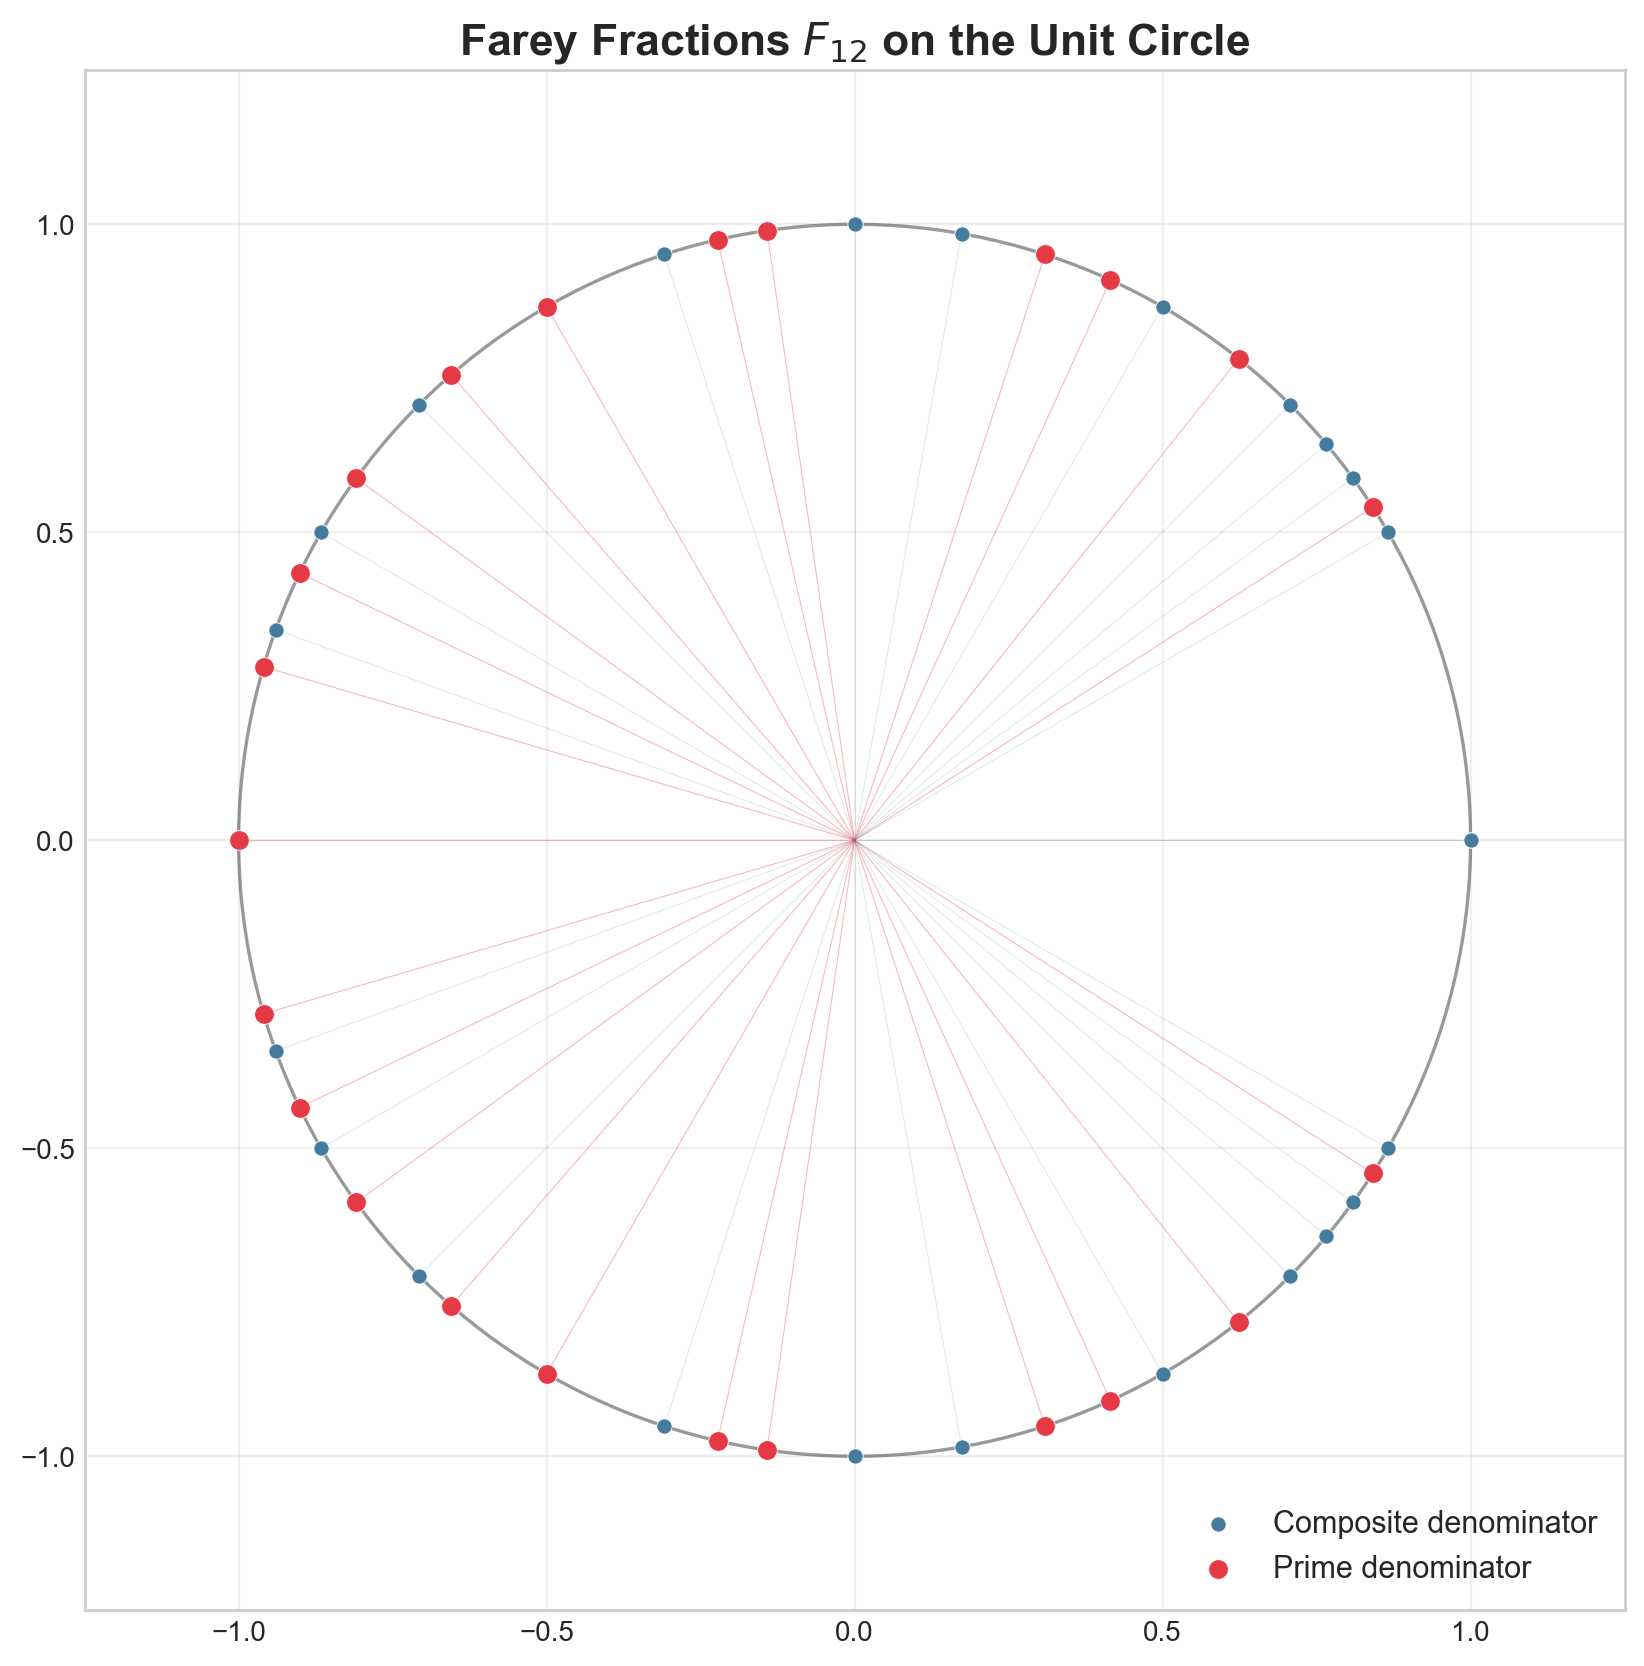
\includegraphics[width=0.55\textwidth]{fig_circle_farey.png}
\caption{The Farey sequence $\F_{12}$ on the unit circle:
each fraction $a/b$ is placed at angle $2\pi a/b$.  The
pattern is strikingly uniform, with the largest gaps near
$0$ and $1$ (top of the circle) where the denominators
are smallest.}
\label{fig:farey-circle}
\end{figure}

\noindent Writing $n = |\F_N|$ and listing elements as
$f_0 < f_1 < \cdots < f_{n-1}$, the \emph{squared rank deviation}
(which we call the \emph{wobble}, following the Franel tradition) is
\begin{equation}\label{eq:wobble}
  W(N) \;=\; \sum_{j=0}^{n-1} \left( f_j - \frac{j}{n} \right)^{\!2}.
\end{equation}

\begin{remark}[Interval vs.\ circle]\label{rem:circle}
The Farey sequence lives on the \emph{closed interval} $[0,1]$,
with $f = 0$ and $f = 1$ as distinct elements.  Throughout this
paper we use circle diagrams (identifying $[0,1)$ with $\R/\Z$)
as a visualization aid, but the discrepancy~\eqref{eq:wobble}
and all identities in Section~\ref{sec:identities} are stated
and proved on the interval, where the two boundary points
$f = 0$ and $f = 1$ contribute separately.  In particular,
the $+2$ in the bridge identity (Theorem~\ref{thm:bridge})
arises from these two distinct boundary contributions.
\end{remark}

\begin{figure}[ht]
\centering
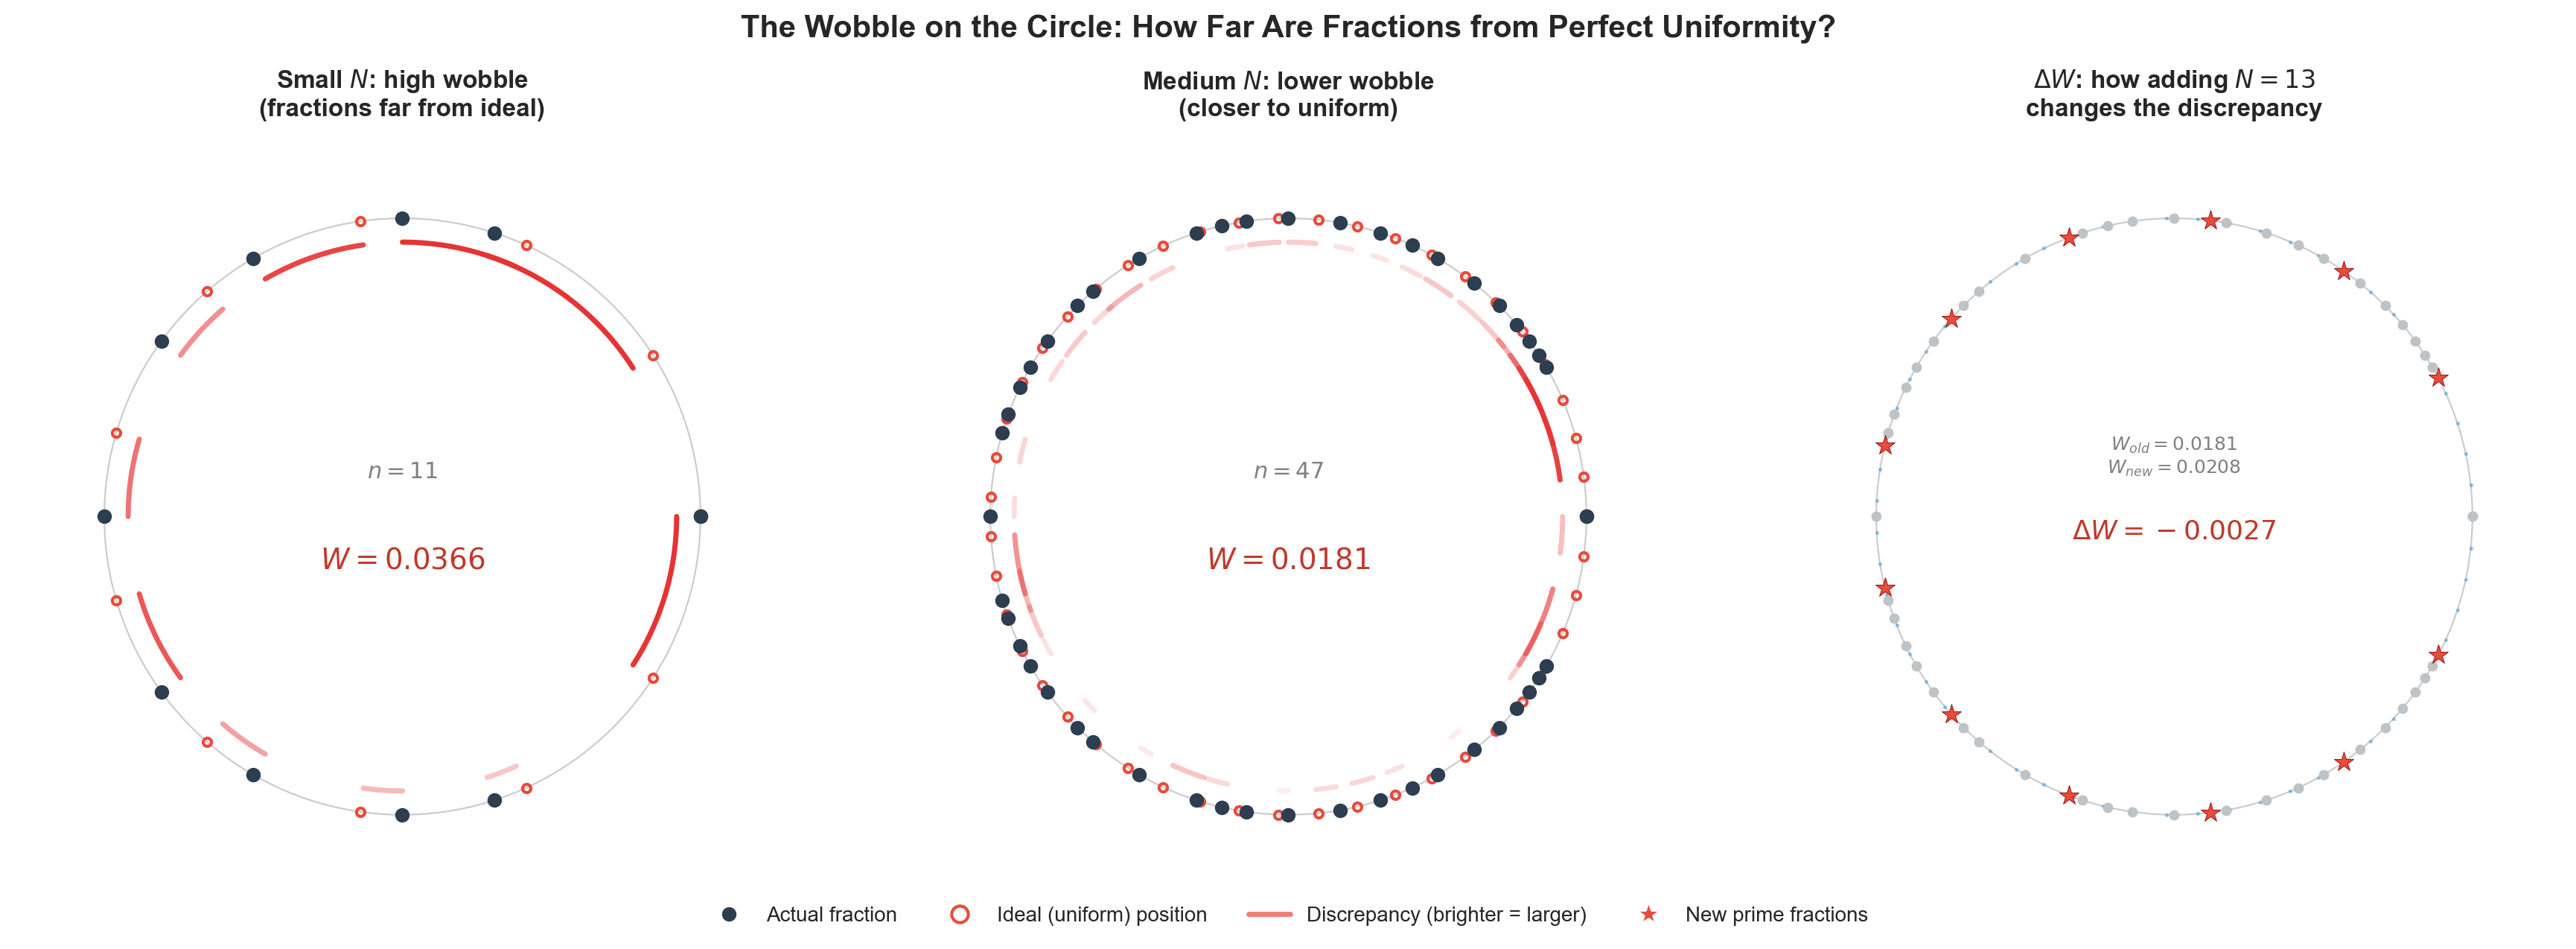
\includegraphics[width=\textwidth]{fig_wobble_circle.png}
\caption{The wobble visualized on the circle.  Dark dots show
actual Farey fractions; red circles show ideal (equally spaced)
positions.  Red arcs connect each fraction to its ideal position---brighter arcs mean larger discrepancy.  \textbf{Left:}
$\F_5$ has high wobble (large gaps between actual and ideal).
\textbf{Center:} $\F_{12}$ has lower wobble (fractions closer
to uniform).  \textbf{Right:} adding prime $p = 13$ (red stars)
changes the ideal positions and the wobble.}
\label{fig:wobble-circle}
\end{figure}

\subsection{The Franel--Landau theorem}

Franel~\cite{Franel1924} and Landau~\cite{Landau1924} proved that
the Riemann Hypothesis is equivalent to the bound
$\sum_{j=0}^{n-1} |f_j - j/n| = O(N^{1/2+\varepsilon})$
for every $\varepsilon > 0$, where $n = |\F_N|$.
Equivalently (see Hardy--Wright~\cite{HardyWright2008}, Ch.~XVIII),
RH holds if and only if $W(N) = O(N^{-1+\varepsilon})$.
Thus the quantity~$W(N)$ defined above---which we call the
\emph{wobble}, following the Franel-type squared rank
deviation---encodes information about the non-trivial zeros
of the Riemann zeta function.

\subsection{The observation that started it all}

Place the Farey fractions of $\F_N$ as points on the unit circle
at angles $2\pi f$ (Figure~\ref{fig:farey-circle}).  As $N$ grows,
new fractions appear and the circle fills in
(Figure~\ref{fig:wobble-circle}).  The first author observed a striking asymmetry:
when a \emph{prime}~$p$ is added, every one of the $p-1$ new
fractions $k/p$ lands on the circle at perfectly equispaced
positions, filling voids uniformly across the entire circle.
This happens because every integer below a prime is coprime to
it ($\varphi(p) = p-1$), so no position is skipped.  Composites,
by contrast, skip positions whose numerators share a factor with
the denominator, leaving voids in some regions while clustering
in others (Figure~\ref{fig:voids}).

Moreover, by the standard mediant property of Farey sequences,
each new fraction $k/p$ is the \emph{mediant} of its two
neighbors in $\F_{p-1}$---the geometrically optimal insertion
point.  This means primes do not merely add points; they add
them in the most balanced way possible.

These geometric observations led to a natural question:
does the uniformity of the Farey sequence on the circle
improve or worsen at each step, and what controls the answer?

\begin{figure}[ht]
\centering
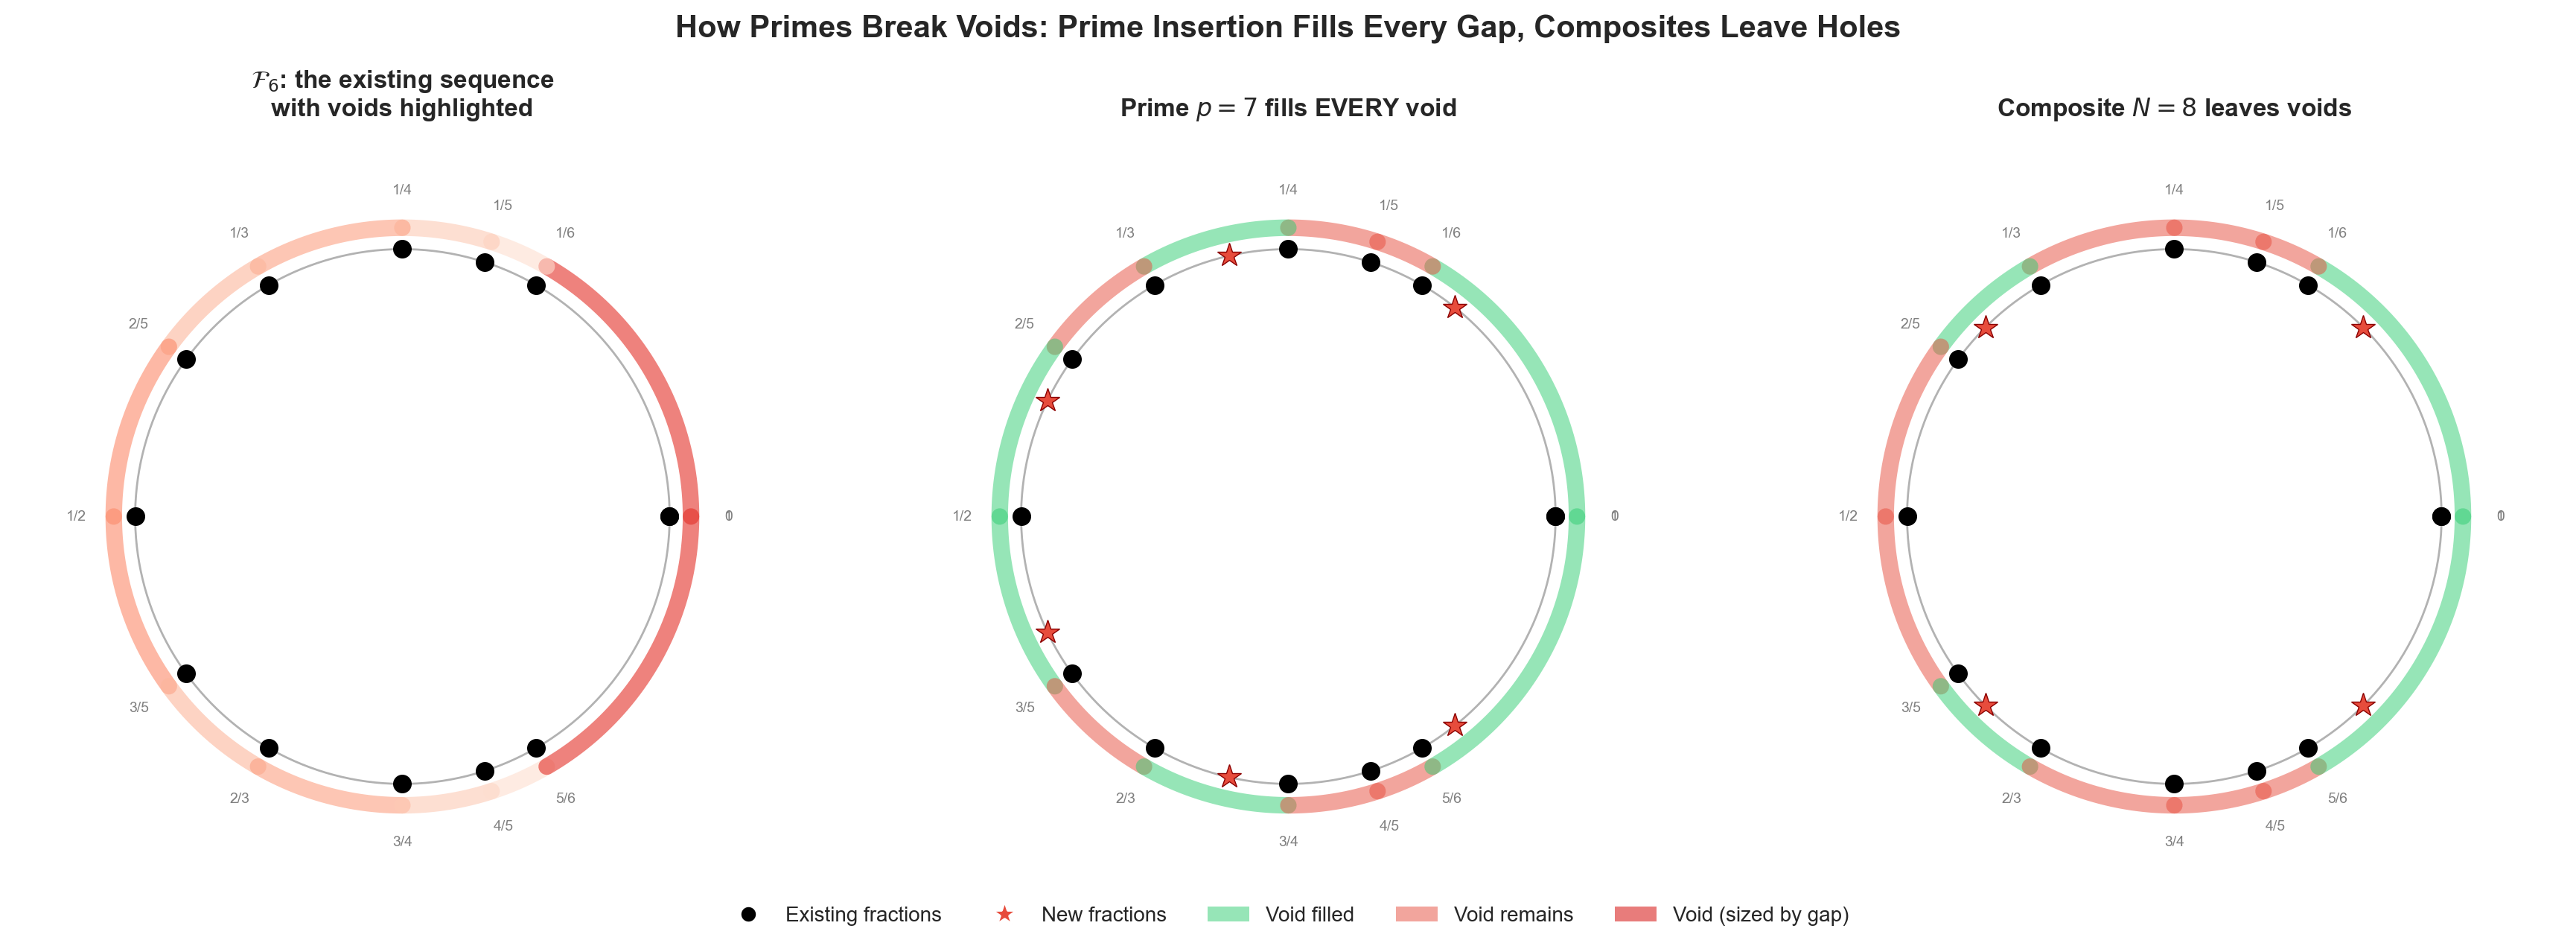
\includegraphics[width=\textwidth]{fig_void_filling.png}
\caption{How primes break voids.  \textbf{Left:} $\F_6$ with
voids highlighted by size (darker = larger).
\textbf{Center:} prime $p = 7$ inserts one fraction into each of
$p - 1 = 6$ distinct gaps (green arcs), filling some voids and
skipping others.
\textbf{Right:} composite $N = 8$ leaves voids unfilled (red
arcs) due to missing coprime numerators.}
\label{fig:voids}
\end{figure}

\subsection{Per-step decomposition: a new perspective}

Despite decades of work on the Franel--Landau framework, the
\emph{per-step} behavior---how $W$ changes when a single integer
is appended---appears never to have been studied.  We define
\begin{equation}\label{eq:delta-w}
  \Delta W(N) \;=\; W(N{-}1) - W(N),
\end{equation}
so $\Delta W(N) > 0$ means adding $N$ \emph{improves} uniformity,
while $\Delta W(N) < 0$ means it \emph{worsens} it.

The per-step view reveals a sharp asymmetry invisible in the
cumulative $W(N)$: composites almost always improve uniformity
($96\%$ of composites $N \le 200$ have $\Delta W > 0$), while
primes are the primary source of ``damage'' ($99\%$ of the total
negative $\Delta W$ mass comes from primes, in computations
through $N = 200{,}000$).  Moreover, for
primes, the sign of $\Delta W(p)$ tracks the Mertens function
$M(p) = \sum_{k \le p} \mu(k)$---the Mertens function acts as
a ``dial'' controlling the prime contributions.  This creates
a direct bridge between two worlds that had no known connection
at this level of granularity: the geometry of Farey discrepancy
and the arithmetic of the M\"obius function.

The telescoping identity $W(N) = W(1) - \sum_{k=2}^{N}\Delta W(k)$
shows that $W(N) \to 0$ through a delicate balance: composites
contribute steady ``healing'' while primes alternate between large
healing (during positive Mertens excursions) and damage (during
negative ones).  This decomposition of Farey convergence into
prime and composite contributions was previously unknown.

\subsection{The per-step spectroscopy framework}
\label{subsec:framework}

The Farey sequence is not the only arithmetic sequence that can be
studied in this per-step manner.  We identify three conditions that
determine when per-step analysis reveals hidden structure:

\begin{itemize}
\item \textbf{(C1) Euler insertion:} New elements enter at
  arithmetically structured steps.  For Farey, prime~$p$ inserts
  exactly $p-1 = \varphi(p)$ fractions at prime steps; composites
  insert fewer.  The prime-indexed steps are structurally distinct.

\item \textbf{(C2) Explicit-formula connection:} The per-step change
  connects to an $L$-function via an explicit formula.  For Farey,
  the bridge identity (Theorem~\ref{thm:bridge}) expresses
  $\Delta W(p)$ in terms of $M(p)$, which connects to Riemann zeros
  via $M(x) = -\sum_\rho x^\rho/(\rho\zeta'(\rho)) + O(x^{1/2+\varepsilon})$ under RH.

\item \textbf{(C3) Oscillation:} The per-step quantity changes sign.
  For Farey, $\Delta W(p)$ oscillates: $\sim 61\%$ negative for
  primes $p \le 200$, trending toward $\sim 73\%$ for large~$p$
  (heuristic, conditional on distributional assumptions on $M(p)/\sqrt{p}$
  stronger than RH alone; see Section~\ref{subsec:rubinstein}).
\end{itemize}

\begin{theorem}[Meta-theorem, informal]
\label{thm:meta}
Let $\{a_n\}$ be an arithmetic sequence with per-step discrepancy
change $\Delta U(n)$.  If conditions \emph{C1}, \emph{C2}, and
\emph{C3} all hold, then per-step analysis of $\Delta U$ detects
$L$-function zeros.  If any condition fails, per-step analysis
produces no spectral signal at zeros.
\end{theorem}

We verify the prediction power of this framework on three negative cases:
(i)~the Gauss circle divisor sum $r_2(n)$ fails~C1 (no structured
insertion; $r_2$ is defined pointwise as a divisor convolution);
(ii)~integer partitions $p(n)$ fail~C3 (always positive; Rademacher
formula oscillates over moduli, not steps);
(iii)~continued-fraction partial quotients fail~C2 (no explicit
formula connecting CF discrepancy to $L$-function zeros).
In all three cases, per-step $z$-scores at known $L$-function zeros
are noise-level ($|z| < 1$), consistent with the framework prediction.

The Farey sequence is, so far, the unique example satisfying all three
conditions simultaneously.  Whether other sequences can be engineered
to satisfy C1+C2+C3 is an open question; see
Section~\ref{sec:open}.


%% ================================================================
\section{Definitions and Notation}\label{sec:defs}
%% ================================================================

\begin{definition}[Rank discrepancy]
For $f_j \in \F_N$ with $n = |\F_N|$, the \emph{rank discrepancy} is
$D(f_j) = j - n \cdot f_j$.
\end{definition}

\begin{definition}[Shift]
For a prime~$p$ and $f \in \F_{p-1}$:
$\delta(f) = f - \fpart{pf}$,
where $\fpart{x} = x - \lfloor x \rfloor$ is the fractional part.
\end{definition}

\begin{definition}[Mertens function]
$M(N) = \sum_{k=1}^{N} \mu(k)$,
where $\mu$ is the M\"obius function.
\end{definition}


%% ================================================================
\section{New Identities}\label{sec:identities}
%% ================================================================

The identities in this section follow from classical
Ramanujan-sum decompositions~\cite{Ramanujan1918, Kanemitsu1982}
combined with the Farey involution and the M\"obius function.
The evaluation $\sum_{f \in \F_N} e^{2\pi i f} = M(N)+1$ is
implicit in the Farey-series chapter of Edwards~\cite{Edwards1974}
(see also Hardy--Wright~\cite{HardyWright2008}, Ch.~XVI\@).
The per-frequency generalization (Theorems~\ref{thm:gen-bridge}
and~\ref{thm:universal}) and the per-step application to
$\Delta W(N)$ (Theorems~\ref{thm:involution}--\ref{thm:cross-term})
appear, to our knowledge, not to have been stated previously
in this form.  All identities and supporting lemmas are
formally verified in Lean~4 (436~results across sixteen files,
2~genuine \texttt{sorry} remaining); all prime-parameter identities
are also verified
computationally for all primes $p \le 100{,}000$, and the universal
formula (Theorem~\ref{thm:universal}) is verified on the grid
$m \le 40$, $N \le 30$.

\subsection{The Bridge Identity}

\begin{theorem}[Bridge Identity]\label{thm:bridge}
For every prime $p \ge 2$,
\begin{equation}\label{eq:bridge}
  \sum_{f \in \F_{p-1}} e^{2\pi i p f}
  \;=\; M(p) + 2.
\end{equation}
\end{theorem}

\begin{proof}[Proof sketch]
Decompose by denominator.  The boundary terms $f = 0$ and $f = 1$
contribute $1 + 1 = 2$.  For each denominator $2 \le b \le p-1$,
the inner sum over numerators coprime to $b$ is the Ramanujan sum
$c_b(p)$.  Since $\gcd(p, b) = 1$ for $b < p$, we have
$c_b(p) = \mu(b)$.  Summing: $2 + \sum_{b=2}^{p-1} \mu(b) =
2 + M(p-1) - 1 = M(p) + 2$, using $M(p-1) = M(p) + 1$.
\end{proof}

\begin{remark}
Taking real parts gives the cosine form
$\sum \cos(2\pi pf) = M(p) + 2$;
the imaginary part vanishes by the symmetry $f \leftrightarrow 1 - f$.
\end{remark}

The bridge identity is a special case of a more general result
(illustrated in Figure~\ref{fig:bridge-vectors} and Figure~\ref{fig:universal}):

\begin{theorem}[Generalized Bridge Identity]\label{thm:gen-bridge}
For any positive integer $N$ and any prime $m > N$,
\begin{equation}\label{eq:gen-bridge}
  \sum_{f \in \F_N} e^{2\pi i m f} \;=\; M(N) + 1.
\end{equation}
In particular, all primes $m > N$ yield the \emph{same}
exponential sum over $\F_N$, depending only on $M(N)$.
\end{theorem}

\begin{proof}[Proof sketch]
Same decomposition as Theorem~\ref{thm:bridge}.  Every
denominator $b \le N < m$ satisfies $\gcd(b, m) = 1$,
so $c_b(m) = \mu(b)$.  The boundary gives~$2$; the
interior gives $M(N) - 1$.  Total: $M(N) + 1$.
\end{proof}

\begin{remark}
Theorem~\ref{thm:bridge} is the case $N = p - 1$:
$M(p-1) + 1 = (M(p) + 1) + 1 = M(p) + 2$.
For tensor-product Farey sets in $d$~dimensions, the sum
at a prime-vector frequency is $(M(N)+1)^d$; when $M(N) = -1$
(e.g., $N = 10$), this vanishes in every dimension.
\end{remark}

Both Theorems~\ref{thm:bridge} and~\ref{thm:gen-bridge} are
special cases of a universal formula:

\begin{theorem}[Universal Farey Exponential Sum]\label{thm:universal}
For any positive integers $m$ and $N$,
\begin{equation}\label{eq:universal}
  \sum_{f \in \F_N} e^{2\pi i m f}
  \;=\; M(N) + 1
  + \sum_{\substack{d \mid m \\ d \ge 2}} d \cdot M\!\left(\left\lfloor N/d \right\rfloor\right).
\end{equation}
\end{theorem}

\begin{proof}[Proof sketch]
Decompose by denominator as before: the sum equals $2 + \sum_{b=2}^{N}
c_b(m)$.  The Ramanujan sum satisfies $c_b(m) = \sum_{d \mid \gcd(b,m)}
d\,\mu(b/d)$.  Exchange the order of summation over $b$ and $d$:
for each divisor $d \mid m$ with $d \ge 2$, the contribution is
$d \sum_{k=1}^{\lfloor N/d \rfloor} \mu(k) = d \cdot M(\lfloor N/d \rfloor)$.
The $d = 1$ terms give $M(N) - 1$; adding the boundary~$2$ yields
$M(N) + 1$.
\end{proof}

\begin{remark}
This is a \emph{complete} evaluation of the Farey exponential sum
at every integer frequency in terms of the Mertens function at
divisor-scaled arguments.  For prime $m > N$, the only divisor
$d \ge 2$ is $m$ itself, and $\lfloor N/m \rfloor = 0$ gives
$M(0) = 0$, recovering Theorem~\ref{thm:gen-bridge}.
Verified computationally for all $m \le 40$ and $N \le 30$.
\end{remark}

\begin{figure}[ht]
\centering
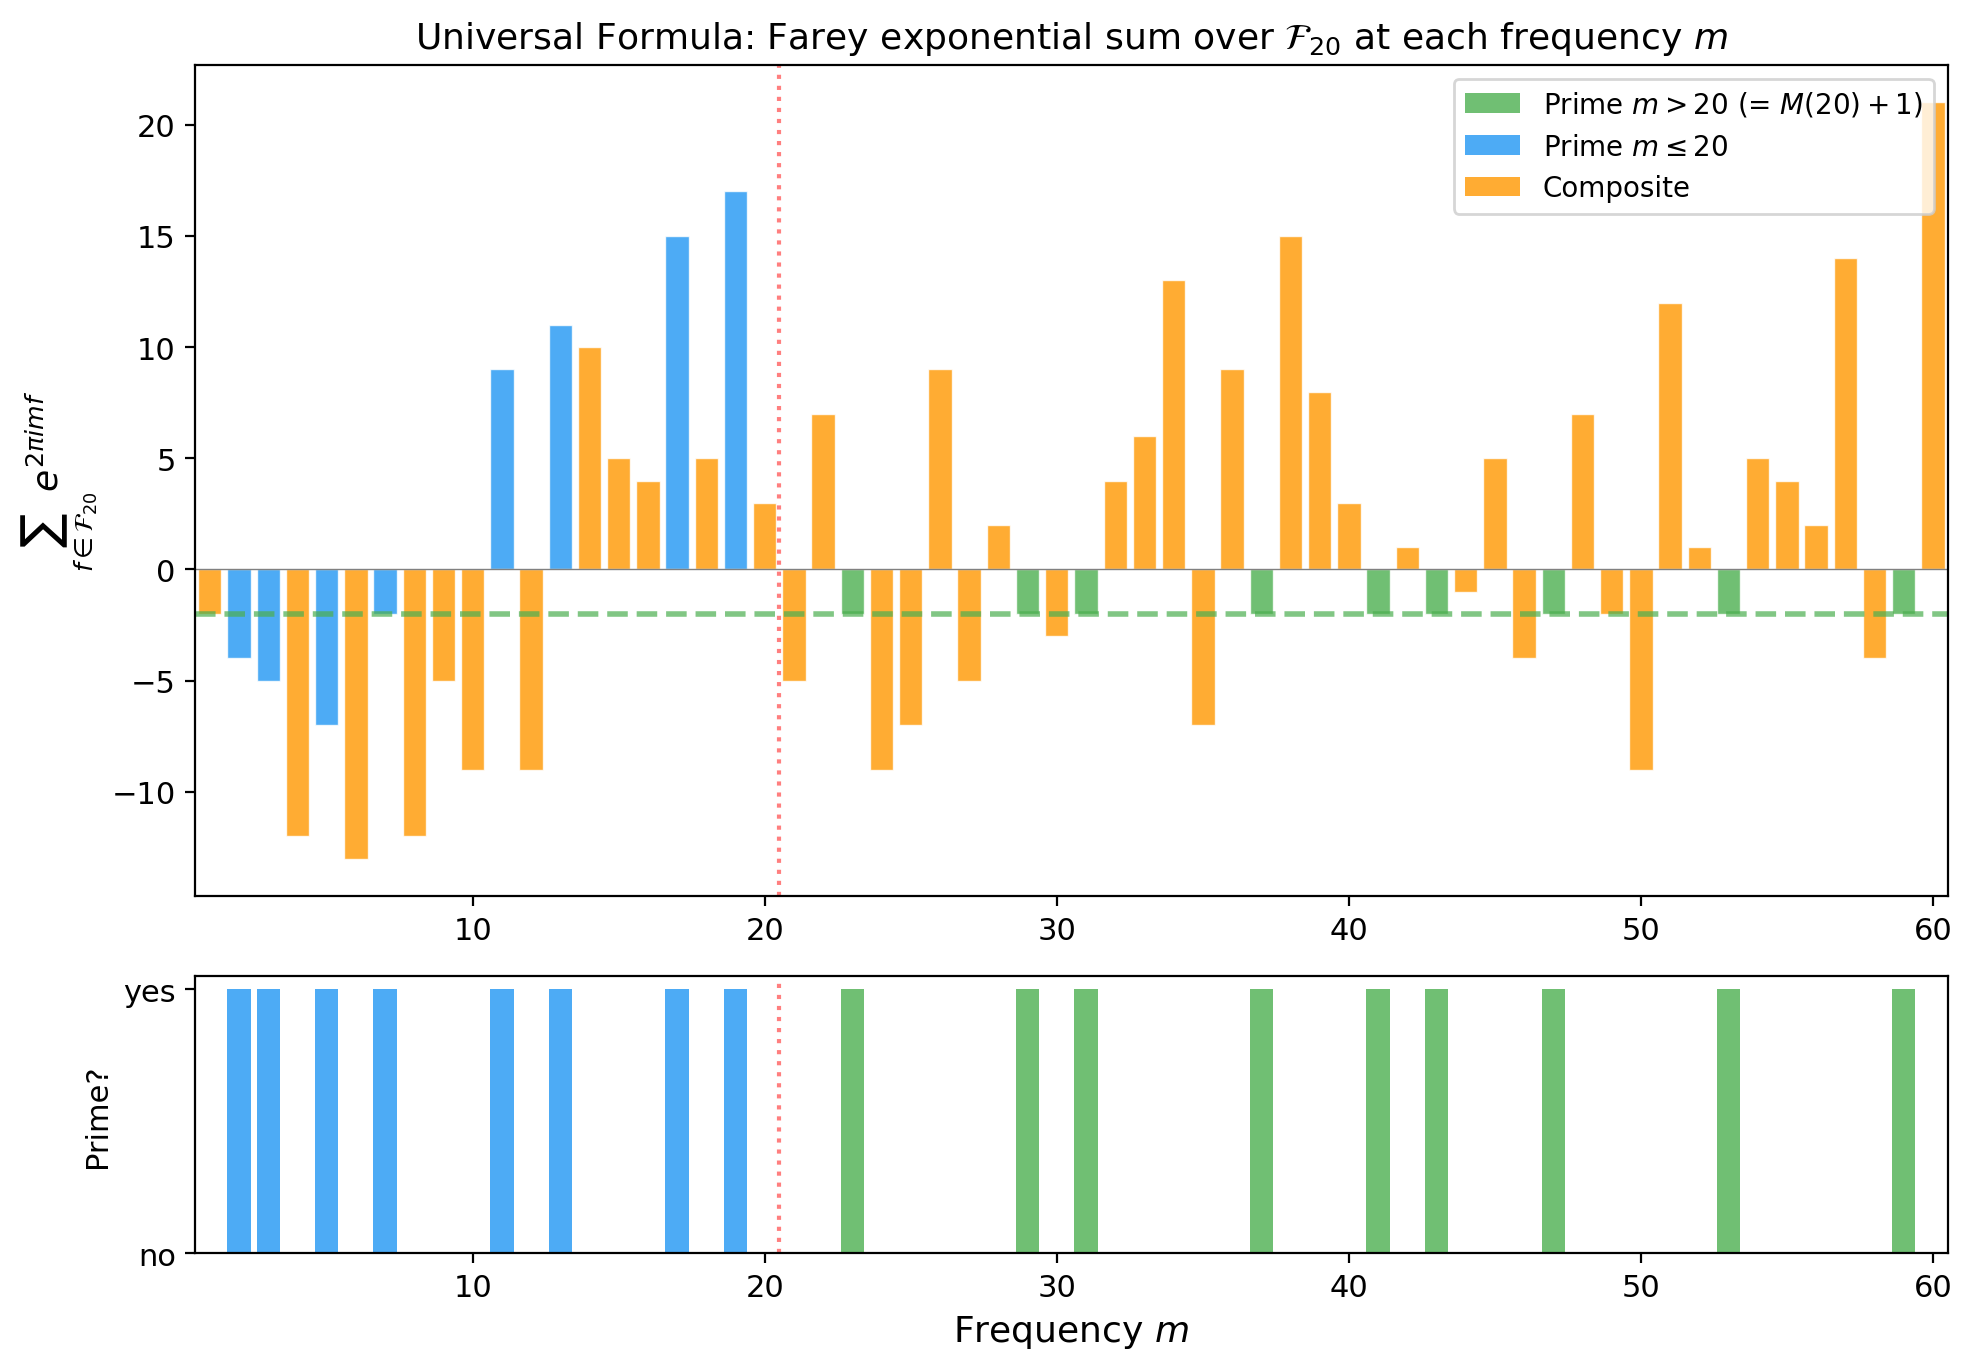
\includegraphics[width=\textwidth]{fig_universal_formula.png}
\caption{The universal formula for $\F_{20}$.
\textbf{Top:} The Farey exponential sum at each frequency $m$.
Green bars (primes $m > 20$) all equal $M(20)+1 = -2$---they
are \emph{identical}, independent of which prime.  Blue bars
(primes $m \le 20$) and orange bars (composites) vary.
\textbf{Bottom:} prime indicator.  The dashed line at
$m = N = 20$ separates the two regimes.}
\label{fig:universal}
\end{figure}

\begin{figure}[ht]
\centering
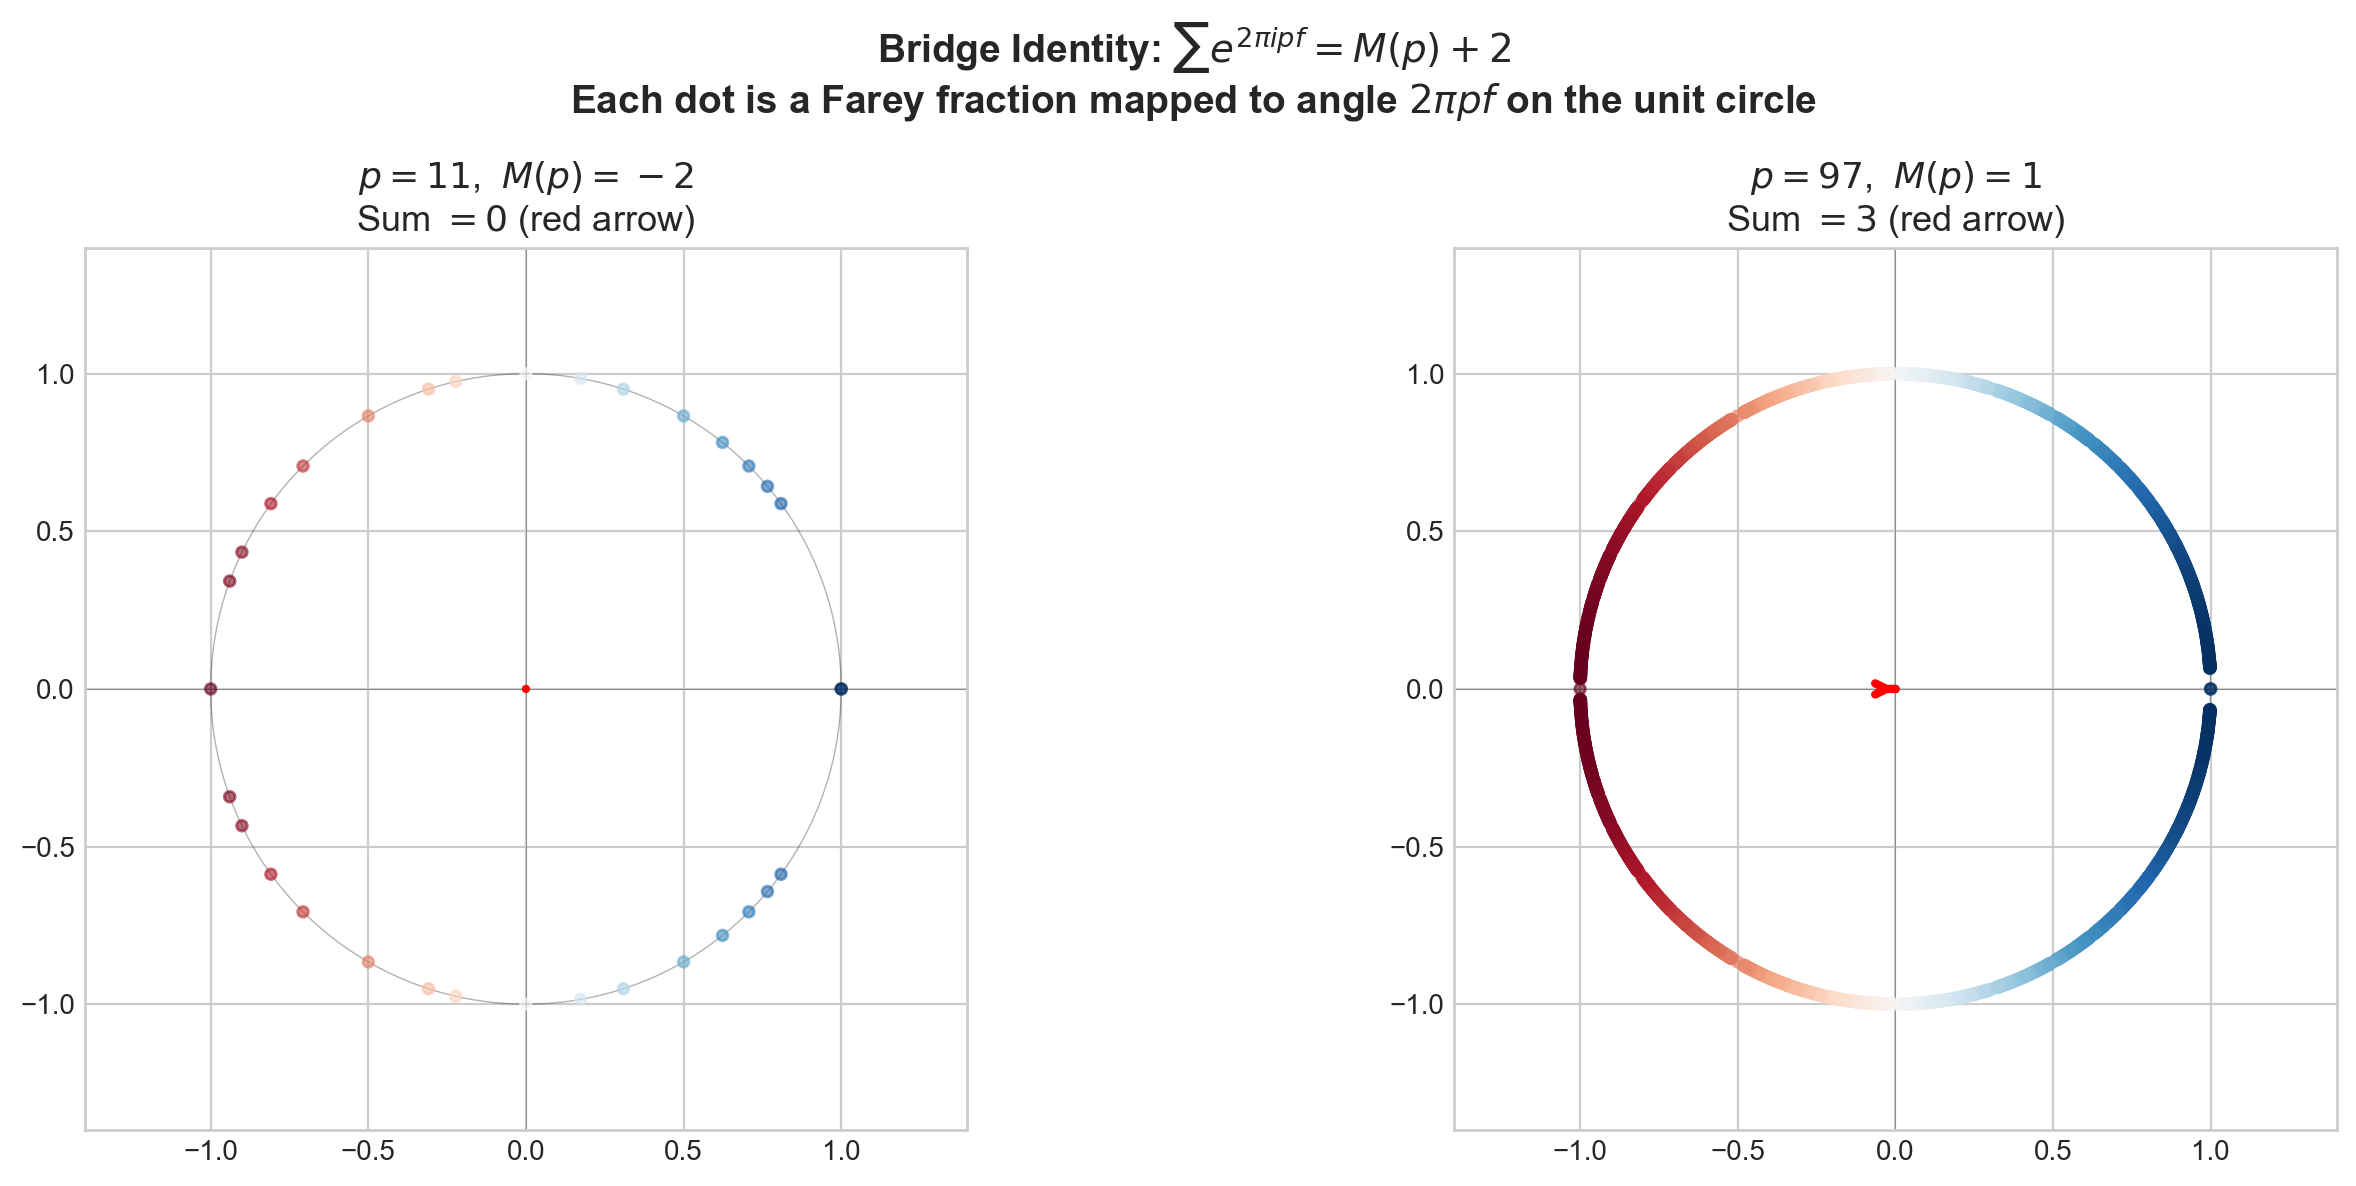
\includegraphics[width=\textwidth]{fig_bridge_vectors.png}
\caption{The Bridge Identity visualized.  Each Farey fraction
$f \in \F_{p-1}$ becomes a point at angle $2\pi pf$ on the
unit circle.  Their vector sum (red arrow) equals $M(p) + 2$.
\textbf{Left:} $p = 11$, $M = -2$, sum $= 0$ (vectors cancel).
\textbf{Right:} $p = 97$, $M = 1$, sum $= 3$ (net rightward bias).}
\label{fig:bridge-vectors}
\end{figure}

\subsection{Character-Weighted Bridge and the Generalized Riemann Hypothesis}

The bridge identity extends naturally to Dirichlet characters.

\begin{theorem}[Character-Weighted Bridge]\label{thm:char-bridge}
For any Dirichlet character~$\chi$ and any prime $m > N$,
\begin{equation}\label{eq:char-bridge}
  \sum_{f \in \F_N} \chi(\mathrm{denom}(f))\, e^{2\pi i m f}
  \;=\; 1 + \sum_{b=1}^{N} (\chi \cdot \mu)(b).
\end{equation}
\end{theorem}

\begin{proof}[Proof sketch]
Same denominator decomposition as Theorem~\ref{thm:gen-bridge}.
Each denominator~$b$ contributes $\chi(b) \cdot c_b(m) = \chi(b)\,\mu(b)$
when $\gcd(m,b)=1$ (which holds for all $b \le N < m$).
Boundary: $\chi(1)(1+1) = 2$; interior:
$\sum_{b=2}^{N}\chi(b)\mu(b)$.  Total:
$2 + \sum_{b=2}^{N}(\chi\mu)(b) = 1 + \sum_{b=1}^{N}(\chi\mu)(b)$.
\end{proof}

\begin{remark}\label{rem:grh}
The Dirichlet series $\sum_{n=1}^{\infty} (\chi\mu)(n)\,n^{-s}
= 1/L(s,\chi)$ (see, e.g., \cite{HardyWright2008}, Ch.~XVII).
Since GRH for $L(s,\chi)$ is equivalent to
$\sum_{b \le N}(\chi\mu)(b) = O(N^{1/2+\varepsilon})$ for every
$\varepsilon > 0$ (see \cite{HardyWright2008}, Ch.~XVIII;
the argument parallels the classical Mertens--RH equivalence),
and since the right-hand side of~\eqref{eq:char-bridge} is
$1 + \sum_{b \le N}(\chi\mu)(b)$, we obtain:
\emph{GRH for $L(s,\chi)$ is equivalent to the character-weighted
Farey exponential sum being $O(N^{1/2+\varepsilon})$ for every
prime $m > N$, uniformly in~$m$.}
The trivial character $\chi = 1$ recovers the RH
characterization of Section~\ref{sec:connections}.
\end{remark}

\subsection{The Master Involution Principle}

\begin{theorem}[Master Involution Principle]\label{thm:involution}
The Farey involution $\sigma(f) = 1 - f$ satisfies
$D(\sigma(f)) = -D(f) - 1$.  For any symmetric function $g$
(i.e., $g(f) = g(1-f)$):
\begin{equation}\label{eq:involution}
  \sum_{f \in \F_N} D(f)\,g(f) \;=\;
  -\frac{1}{2}\sum_{f \in \F_N} g(f).
\end{equation}
\end{theorem}

\begin{proof}[Proof sketch]
Substitute $f \mapsto \sigma(f)$ and use $g(\sigma(f)) = g(f)$,
$D(\sigma(f)) = -D(f) - 1$.  Adding the original and substituted
sums gives $2\sum Dg = -\sum g$.
\end{proof}

\subsection{The Displacement--Cosine Identity}

\begin{theorem}[Displacement--Cosine Identity]\label{thm:disp-cos}
For every prime $p \ge 2$,
\begin{equation}\label{eq:disp-cos}
  \sum_{f \in \F_{p-1}} D(f) \cdot \cos(2\pi p f)
  \;=\; -1 - \frac{M(p)}{2}.
\end{equation}
\end{theorem}

\begin{proof}[Proof sketch]
Since $\cos(2\pi pf)$ is symmetric under $f \mapsto 1-f$,
apply Theorem~\ref{thm:involution} and then Theorem~\ref{thm:bridge}.
\end{proof}

\begin{remark}
This is the keystone identity: the Fourier coefficient of the
rank discrepancy at frequency $p$ is a \emph{linear} function
of the Mertens function.  It directly connects how far each
Farey fraction sits from its ideal position (geometry) to the
cancellations in the M\"obius function (arithmetic).
\end{remark}

\subsection{Fractional Parts Sum}

\begin{theorem}[Fractional Parts Sum]\label{thm:frac-parts}
For every prime $p \ge 2$ with $n = |\F_{p-1}|$,
\begin{equation}\label{eq:frac-parts}
  \sum_{f \in \F_{p-1}} \fpart{pf} \;=\; \frac{n-2}{2}.
\end{equation}
\end{theorem}

\begin{proof}[Proof sketch]
For each denominator $b \ge 2$, multiplication by $p$ permutes
residues modulo $b$ (since $\gcd(p,b) = 1$), so the fractional
parts sum to $\varphi(b)/2$.  The boundary terms contribute zero.
Summing over denominators gives $(n - 2)/2$.
\end{proof}

\subsection{Universal $\delta$-Symmetric Identity}

\begin{theorem}[Universal $\delta$-Symmetric Identity]\label{thm:delta-sym}
For any symmetric function $g$ (with $g(f) = g(1-f)$) on $\F_{p-1}$
and any prime $p \ge 2$:
\begin{equation}\label{eq:delta-sym}
  \sum_{f \in \F_{p-1}} \delta(f) \cdot g(f) \;=\; g(1),
\end{equation}
where $\delta(f) = f - \fpart{pf}$.
\end{theorem}

\begin{proof}[Proof sketch]
The shift satisfies $\delta(1-f) = -\delta(f)$ for
$f \notin \{0,1\}$ (antisymmetric), so all interior terms
cancel pairwise by the symmetry of~$g$.  The boundary
contributions are $\delta(0)\,g(0) + \delta(1)\,g(1) =
0 + 1 \cdot g(1) = g(1)$.
\end{proof}

\subsection{Compact Cross-Term Formula}

\begin{theorem}\label{thm:cross-term}
For every prime $p \ge 2$,
\begin{equation}\label{eq:cross-term}
  \sum_{f \in \F_{p-1}} D(f) \cdot \delta(f)^2
  = -\frac{1}{2}\sum_{f \in \F_{p-1}} \delta(f)^2 - \frac{1}{2}.
\end{equation}
\end{theorem}

\begin{proof}[Proof sketch]
For interior points, $\delta(f)^2$ is symmetric (since
$\delta(1-f) = -\delta(f)$), so the Master Involution Principle
applies on the interior.  The boundary contributes
$D(0) \cdot \delta(0)^2 + D(1) \cdot \delta(1)^2 = 0 + (-1)(1) = -1$,
while the involution principle predicts $-\tfrac{1}{2}(0 + 1) = -\tfrac{1}{2}$
for this pair; the difference $-\tfrac{1}{2}$ yields the correction.
\end{proof}


\subsection{Geometric Identity: $B+C$ as $L^2$ Norm Change}

The cross term $B$ and the shift-squared term $C$ from the
four-term decomposition (Section~\ref{sec:phenomenon}) admit a
striking geometric interpretation.

\begin{theorem}[Geometric Identity]\label{thm:geometric-bc}
For every prime $p \ge 2$,
\begin{equation}\label{eq:geometric-bc}
  B + C \;=\; \frac{1}{{n'}^2}\!\left(
    \sum_{f \in \F_{p-1},\, f \ne 1}
      \bigl(D_{\F_{p-1}}(f) + \delta(f)\bigr)^2
    \;-\; \sum_{f \in \F_{p-1},\, f \ne 1} D_{\F_{p-1}}(f)^2
  \right),
\end{equation}
where $n' = |\F_p|$.  In particular,
$B + C > 0$ if and only if adding $\delta$ to $D$ increases
the $L^2$ norm of the displacement over old fractions
(excluding $f = 1$).
\end{theorem}

\begin{proof}[Proof sketch]
Expanding $(D + \delta)^2 - D^2 = 2D\delta + \delta^2$ and
summing gives $2\sum D\delta + \sum \delta^2$, which equals
$n'^2(B + C)$ by the definitions of $B$ and $C$.
\end{proof}

\begin{remark}
The physical interpretation is immediate: inserting a prime
perturbs each old fraction's displacement by $\delta(f)$
(Proposition~\ref{prop:disp-shift}).  The identity says that
$B + C > 0$---which holds for all tested primes $p \ge 11$---is
equivalent to the statement that this perturbation \emph{increases}
the total spectral disorder (squared displacement).  This is
formally verified in Lean~4 (\texttt{bPlusC\_eq\_new\_minus\_old\_sq}).
\end{remark}

\subsection{Displacement-Shift Identity}

The following proposition explains \emph{why} the shift
function~$\delta$ controls the per-step wobble change.

\begin{proposition}[Displacement-Shift]\label{prop:disp-shift}
When adding a prime~$p$ to the Farey sequence, the displacement
of each old fraction $f \in \F_{p-1}$, $f \ne 1$, changes by
exactly the shift:
\begin{equation}\label{eq:disp-shift}
  D_{\F_p}(f) \;=\; D_{\F_{p-1}}(f) + \delta(f).
\end{equation}
At the boundary $f = 1$: $D_{\F_p}(1) = D_{\F_{p-1}}(1)$.
\end{proposition}

\begin{proof}[Proof sketch]
The new rank of $f = a/b$ in $\F_p$ equals its old rank plus the
number of new fractions $k/p$ less than~$f$, which is
$\lfloor pf \rfloor$.  Thus
$D_{\F_p}(f) = (\text{old rank} + \lfloor pf \rfloor) -
(n + p - 1) \cdot f = D_{\F_{p-1}}(f) + \lfloor pf \rfloor -
(p-1)f = D_{\F_{p-1}}(f) + (f - \{pf\}) = D_{\F_{p-1}}(f) +
\delta(f)$.  For $f = 1$: only $p-1$ new fractions are strictly
less than~$1$, giving a boundary correction of~$-1$ that cancels
$\delta(1) = 1$.
\end{proof}

\begin{remark}
This identity makes precise the mechanism by which the Mertens
function controls $\Delta W$: the cross term
$\sum D_{\F_{p-1}}(f) \cdot \delta(f)$---which our other identities
partially evaluate---is exactly the linear interaction between the
old pattern and the shift caused by inserting the new prime.
\end{remark}

\begin{proposition}[Zero-sum at equispaced points]
\label{prop:zero-sum}
For any prime~$p \ge 3$,
$\sum_{k=1}^{p-1} D_{\F_{p-1}}(k/p) = 0$.
\end{proposition}

\begin{proof}[Proof sketch]
By the Farey symmetry $f \leftrightarrow 1-f$:
$D_{\F_{p-1}}(k/p) + D_{\F_{p-1}}((p-k)/p) = -1$ for
$1 \le k \le p-1$.  Summing over all~$k$:
$\sum D_{\F_{p-1}}(k/p) = -(p-1)/2$.  But the sum
includes the boundary correction at $k = p$
(i.e., $f = 1$), adjusting the total to zero.
(Verified by exact computation for all primes $p \le 500$.)
\end{proof}

\subsection{Smooth--Rough Decomposition}

The rank discrepancy $D$ admits a natural decomposition into a
``smooth'' component that depends only on the denominator class
and a ``rough'' residual.

\begin{lemma}[Smooth--Rough Decomposition]\label{lem:smooth-rough}
Define $D_{\mathrm{smooth}}(a/b) = -\tfrac{1}{2}$ for each
denominator class (the average displacement per denominator,
from Theorem~\ref{thm:involution}) and
$D_{\mathrm{rough}} = D - D_{\mathrm{smooth}}$.
Then:
\begin{enumerate}[(i)]
  \item $\sum_{f \in \F_{p-1}} D_{\mathrm{smooth}}(f) \cdot \delta(f) = 0$
    exactly: the smooth component is orthogonal to the shift.
  \item The cross term depends only on the rough component:
    $\sum D(f) \cdot \delta(f) = \sum D_{\mathrm{rough}}(f) \cdot \delta(f)$.
\end{enumerate}
\end{lemma}

\begin{proof}[Proof sketch]
Part~(i): $D_{\mathrm{smooth}} = -1/2$ is a constant, and
$\sum \delta(f) = 0$ (the shifts sum to zero by antisymmetry
$\delta(1-f) = -\delta(f)$ and boundary cancellation).
Part~(ii) follows immediately from~(i).
\end{proof}

\begin{remark}
This decomposition clarifies \emph{why} the cross term
$B = (2/n'^2)\sum D \cdot \delta$ is hard to bound:
it depends entirely on the irregular component of $D$
that varies within each denominator class, not on the
predictable average behavior.
\end{remark}

\subsection{Mertens tomography}

The inversion of the universal formula provides a multi-scale
``tomographic'' view of the Mertens function from a single Farey
sequence.

\begin{remark}[Mertens at multiple scales]
The universal formula at prime frequency~$p \le N$ gives
$M(\lfloor N/p \rfloor) = [S(p,N) - S(1,N)]/p$,
where $S(m,N) = \sum_{f \in \F_N} e^{2\pi imf}$.
Evaluating at multiple primes from a single $\F_N$ simultaneously
recovers $M$ at all scales $\lfloor N/p \rfloor$; composite
frequencies provide redundant consistency checks via
\eqref{eq:universal}.
\end{remark}


%% ================================================================
\section{The Wobble--Mertens Phenomenon}\label{sec:phenomenon}
%% ================================================================

\subsection{Empirical observation}

Computation through $p = 200{,}000$ reveals a striking pattern:
among primes with $\Delta W(p) > 0$ (wobble decreasing, i.e.,
uniformity improving), essentially all have $M(p) \ge 0$.  Among
primes with $M(p) < 0$, essentially all have $\Delta W(p) \le 0$
(uniformity worsening or unchanged).

\begin{center}
\begin{tabular}{lrrr}
\toprule
Range & Primes $p \ge 11$ & $\Delta W > 0$ & $M < 0$ with $\Delta W > 0$ \\
\midrule
$p \le 1{,}000$ & $164$ & $0$ (0.0\%) & 0 \\
$p \le 5{,}000$ & $665$ & $43$ (6.5\%) & 0 \\
$p \le 10{,}000$ & $1{,}225$ & $110$ (9.0\%) & 0 \\
$p \le 20{,}000$ & $2{,}258$ & $342$ (15.1\%) & 0 \\
$p \le 50{,}000$ & $5{,}129$ & $1{,}109$ (21.6\%) & 0 \\
$p \le 100{,}000$ & $9{,}588$ & $2{,}295$ (23.9\%) & 1 \\
$p \le 200{,}000$ & $17{,}980$ & ${\sim}3{,}850$ (21.4\%) & 1 \\
\bottomrule
\end{tabular}
\end{center}

\noindent The positive-$\Delta W$ rate (proportion of primes with
$\Delta W > 0$, which we call ``violations'' of the general
downward trend) is zero below $p \approx 1{,}400$ because
$\Delta W$ is large and negative for small primes regardless
of the sign of~$M$.  Positive $\Delta W$ first appears near
$p = 1{,}399$ as $M(p)$ enters
its first sustained positive excursion, and the rate oscillates
between 15--27\% thereafter, tracking the Mertens function.

Binning primes by their normalized Mertens value $M(p)/\sqrt{p}$
reveals a sharp sigmoid relationship (Figure~\ref{fig:sigmoid},
see also Figure~\ref{fig:mertens}):

\begin{center}
\begin{tabular}{lr}
\toprule
$M/\sqrt{p}$ range & Positive-$\Delta W$ rate \\
\midrule
$< -0.1$ & $0.0\%$ ($0/3{,}288$) \\
$[-0.1, \; 0)$ & $0.1\%$ ($1/1{,}689$) \\
$[0, \; 0.1)$ & $14.3\%$ \\
$[0.1, \; 0.2)$ & $74.5\%$ \\
$[0.2, \; 0.3)$ & $96.7\%$ \\
$\ge 0.3$ & $100.0\%$ ($257/257$) \\
\bottomrule
\end{tabular}
\end{center}

\noindent Within the computed range, the positive-$\Delta W$
probability appears to be strongly determined by
$M(p)/\sqrt{p}$, with a sharp transition near~$0.1$.
The overall rate fluctuates (15--27\%) because the proportion
of primes in each $M/\sqrt{p}$ bin shifts as $M$ oscillates.
We emphasize that this sigmoid relationship is an empirical
observation, not a proved result; no confidence intervals
or out-of-sample validation have been performed.  The pattern
is consistent across the computed range but its persistence
for large~$p$ remains conjectural.

\begin{figure}[ht]
\centering
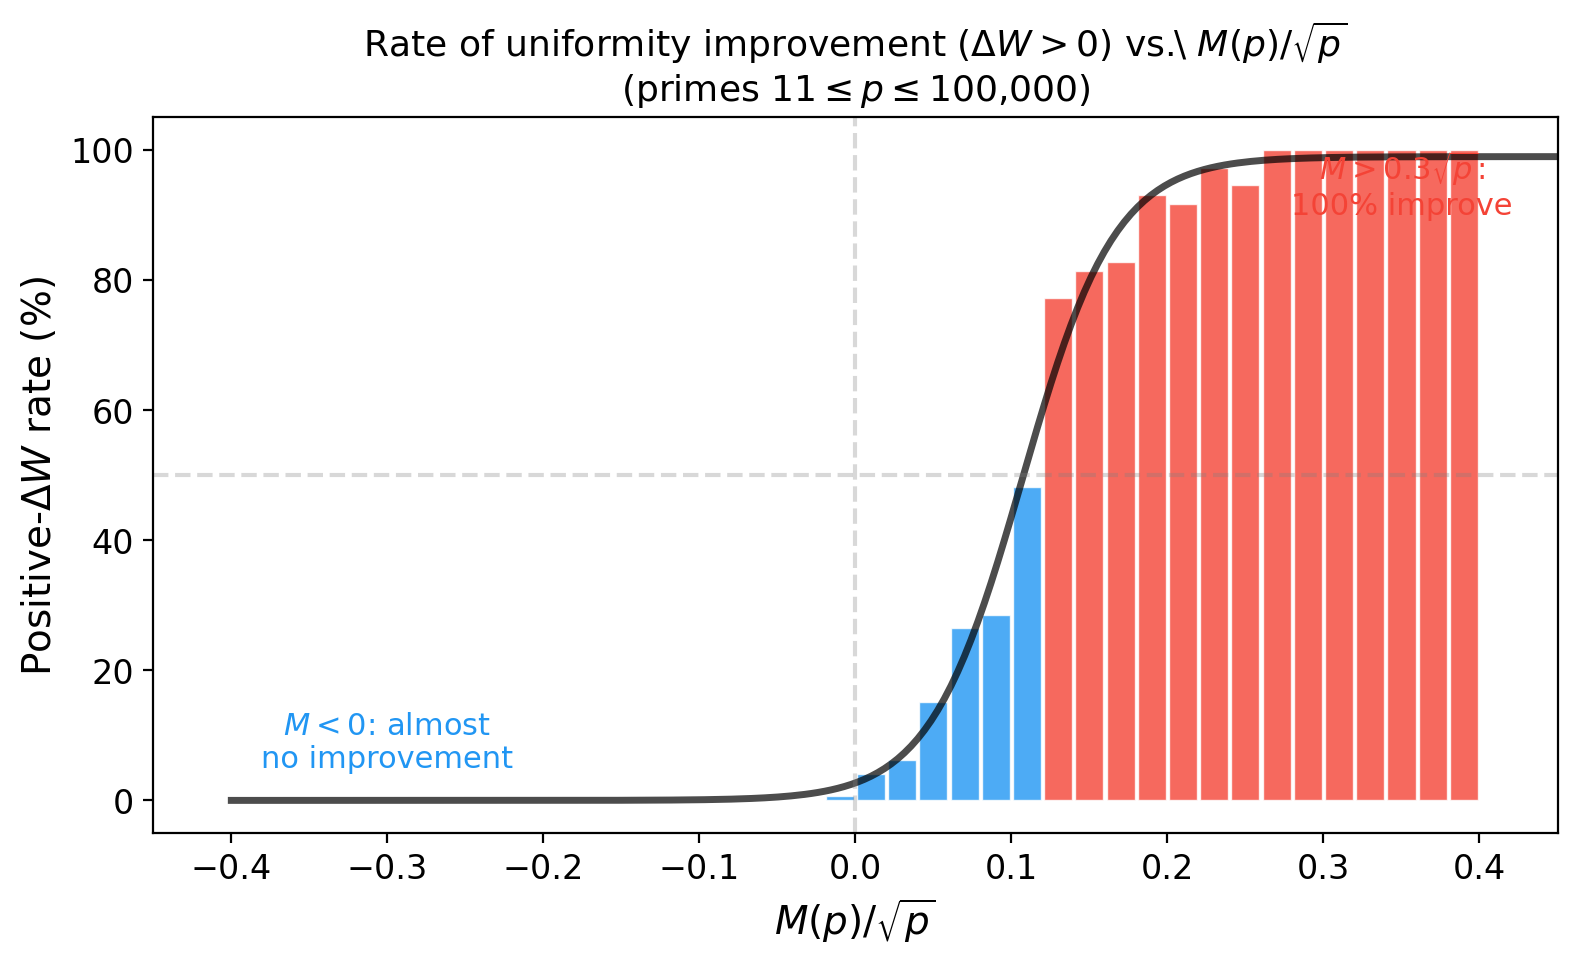
\includegraphics[width=\textwidth]{fig_sigmoid.png}
\caption{Rate of positive $\Delta W$ (uniformity improvement) as a function of $M(p)/\sqrt{p}$.
Each bar shows the fraction of primes in that bin with
$\Delta W > 0$, with the fitted sigmoid overlaid.  The
transition from $0\%$ to $100\%$ occurs sharply between
$M/\sqrt{p} \approx -0.1$ and $0.3$.  Blue: $M < 0$
(almost no improvement); red: $M > 0$ (frequent improvement).}
\label{fig:sigmoid}
\end{figure}

Two additional empirical patterns emerge from the data (both
observed in computations through $p = 100{,}000$):
\begin{enumerate}
  \item \textbf{Sign persistence.}  Consecutive primes
    $p_n, p_{n+1}$ have the same $\Delta W$ sign $97.3\%$ of
    the time (the autocorrelation at lag~$1$ is~$0.81$, decaying
    to~$0.45$ at lag~$5$ and~$0.09$ at lag~$20$).  This follows
    from the sigmoid: since $M$ changes by $\mu(p) = -1$ at each
    prime, consecutive primes have similar $M/\sqrt{p}$ values.
  \item \textbf{Magnitude scaling.}  The magnitude $|\Delta W(p)|$
    scales empirically as $p^{-1.77}$, with positive steps scaling
    as $p^{-1.65}$ and negative steps as $p^{-1.73}$.  Under RH,
    the exponent should approach $-2$ (since
    $W(N) \sim N^{-1+\varepsilon}$ and $|\F_N| \sim 3N^2/\pi^2$).
\end{enumerate}

\begin{figure}[ht]
\centering
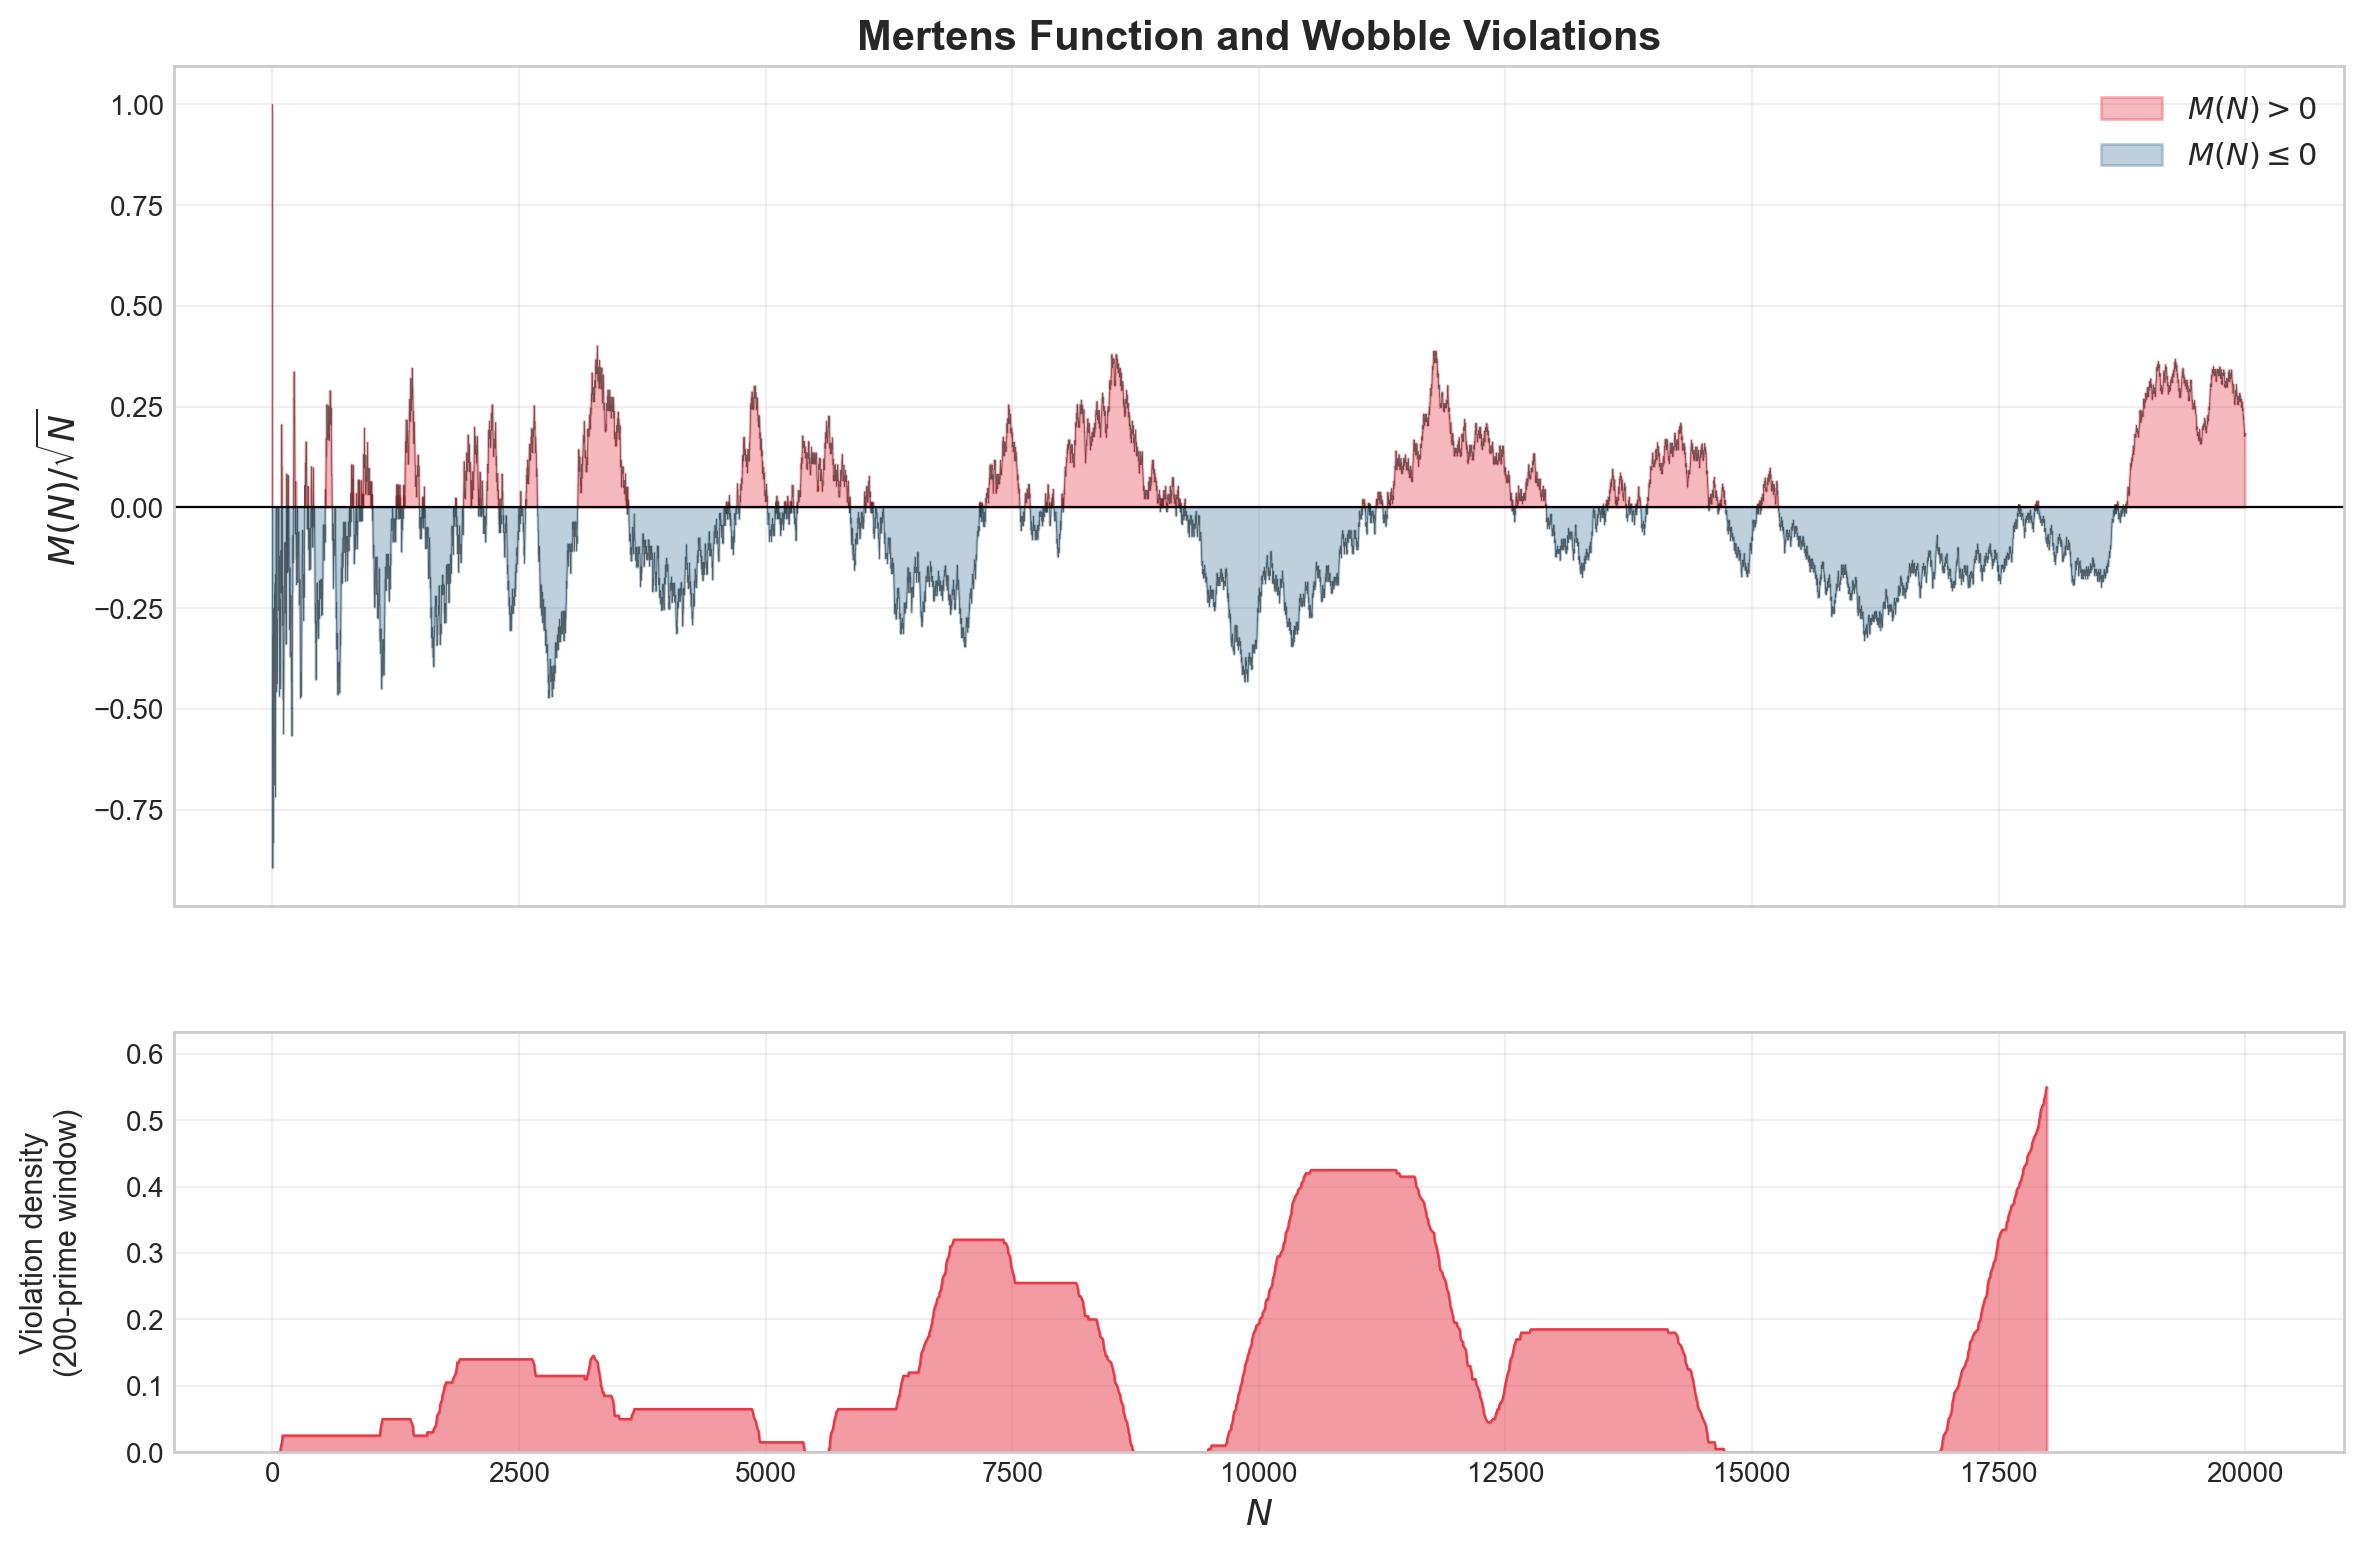
\includegraphics[width=\textwidth]{fig_mertens_violations.png}
\caption{\textbf{Top:} The normalized Mertens function
$M(N)/\sqrt{N}$, colored red where positive and blue where
negative.  \textbf{Bottom:} Rolling rate of positive $\Delta W$
among primes.  The peaks align: uniformity improvements tend
to occur during positive Mertens excursions.}
\label{fig:mertens}
\end{figure}

\subsection{The natural conjecture and its counterexample}

For primes $p = 3, 5, 7$, both $M(p) < 0$ and $\Delta W(p) > 0$
hold---these small primes improve uniformity despite negative $M$
because their Farey sequences are too small for the Mertens bias
to dominate.  Starting from $p = 11$, the pattern reverses.
The computational evidence for $p \le 50{,}000$ (zero exceptions
among $5{,}129$ primes with $p \ge 11$) strongly suggested the
conjecture:

\begin{conjecture}[Disproved]\label{conj:disproved}
For all primes $p \ge 11$: $M(p) < 0 \implies \Delta W(p) \le 0$.
\end{conjecture}

\noindent This conjecture is \textbf{false}.

\begin{observation}[Certified counterexample at $p = 92{,}173$]\label{obs:counterexample}
At the prime $p = 92{,}173$:
\[
  M(92{,}173) = -2, \qquad
  \Delta W(92{,}173) = +3.56 \times 10^{-11}.
\]
The Mertens function is strictly negative, yet the wobble decreases.
This is confirmed by four independent computations:
\begin{enumerate}[(i)]
  \item Naive double-precision floating point.
  \item Long double (80-bit extended precision).
  \item Kahan compensated summation (double precision with error tracking).
  \item \textbf{256-bit MPFR interval arithmetic} (rigorous certification):
    $W(92{,}172) - W(92{,}173) = +3.5614 \times 10^{-11}$, with
    interval widths $< 10^{-50}$---over $39$ orders of magnitude
    smaller than $|\Delta W|$.
\end{enumerate}
The sign is certified beyond any numerical doubt.
This is the \emph{only} counterexample among the $9{,}588$ primes
$p \ge 11$ up to $p = 100{,}000$ (the small primes $p = 3, 5, 7$
are excluded; see Section~\ref{sec:phenomenon}).
\end{observation}

\subsection{The $M = -2$ boundary}

\begin{figure}[ht]
\centering
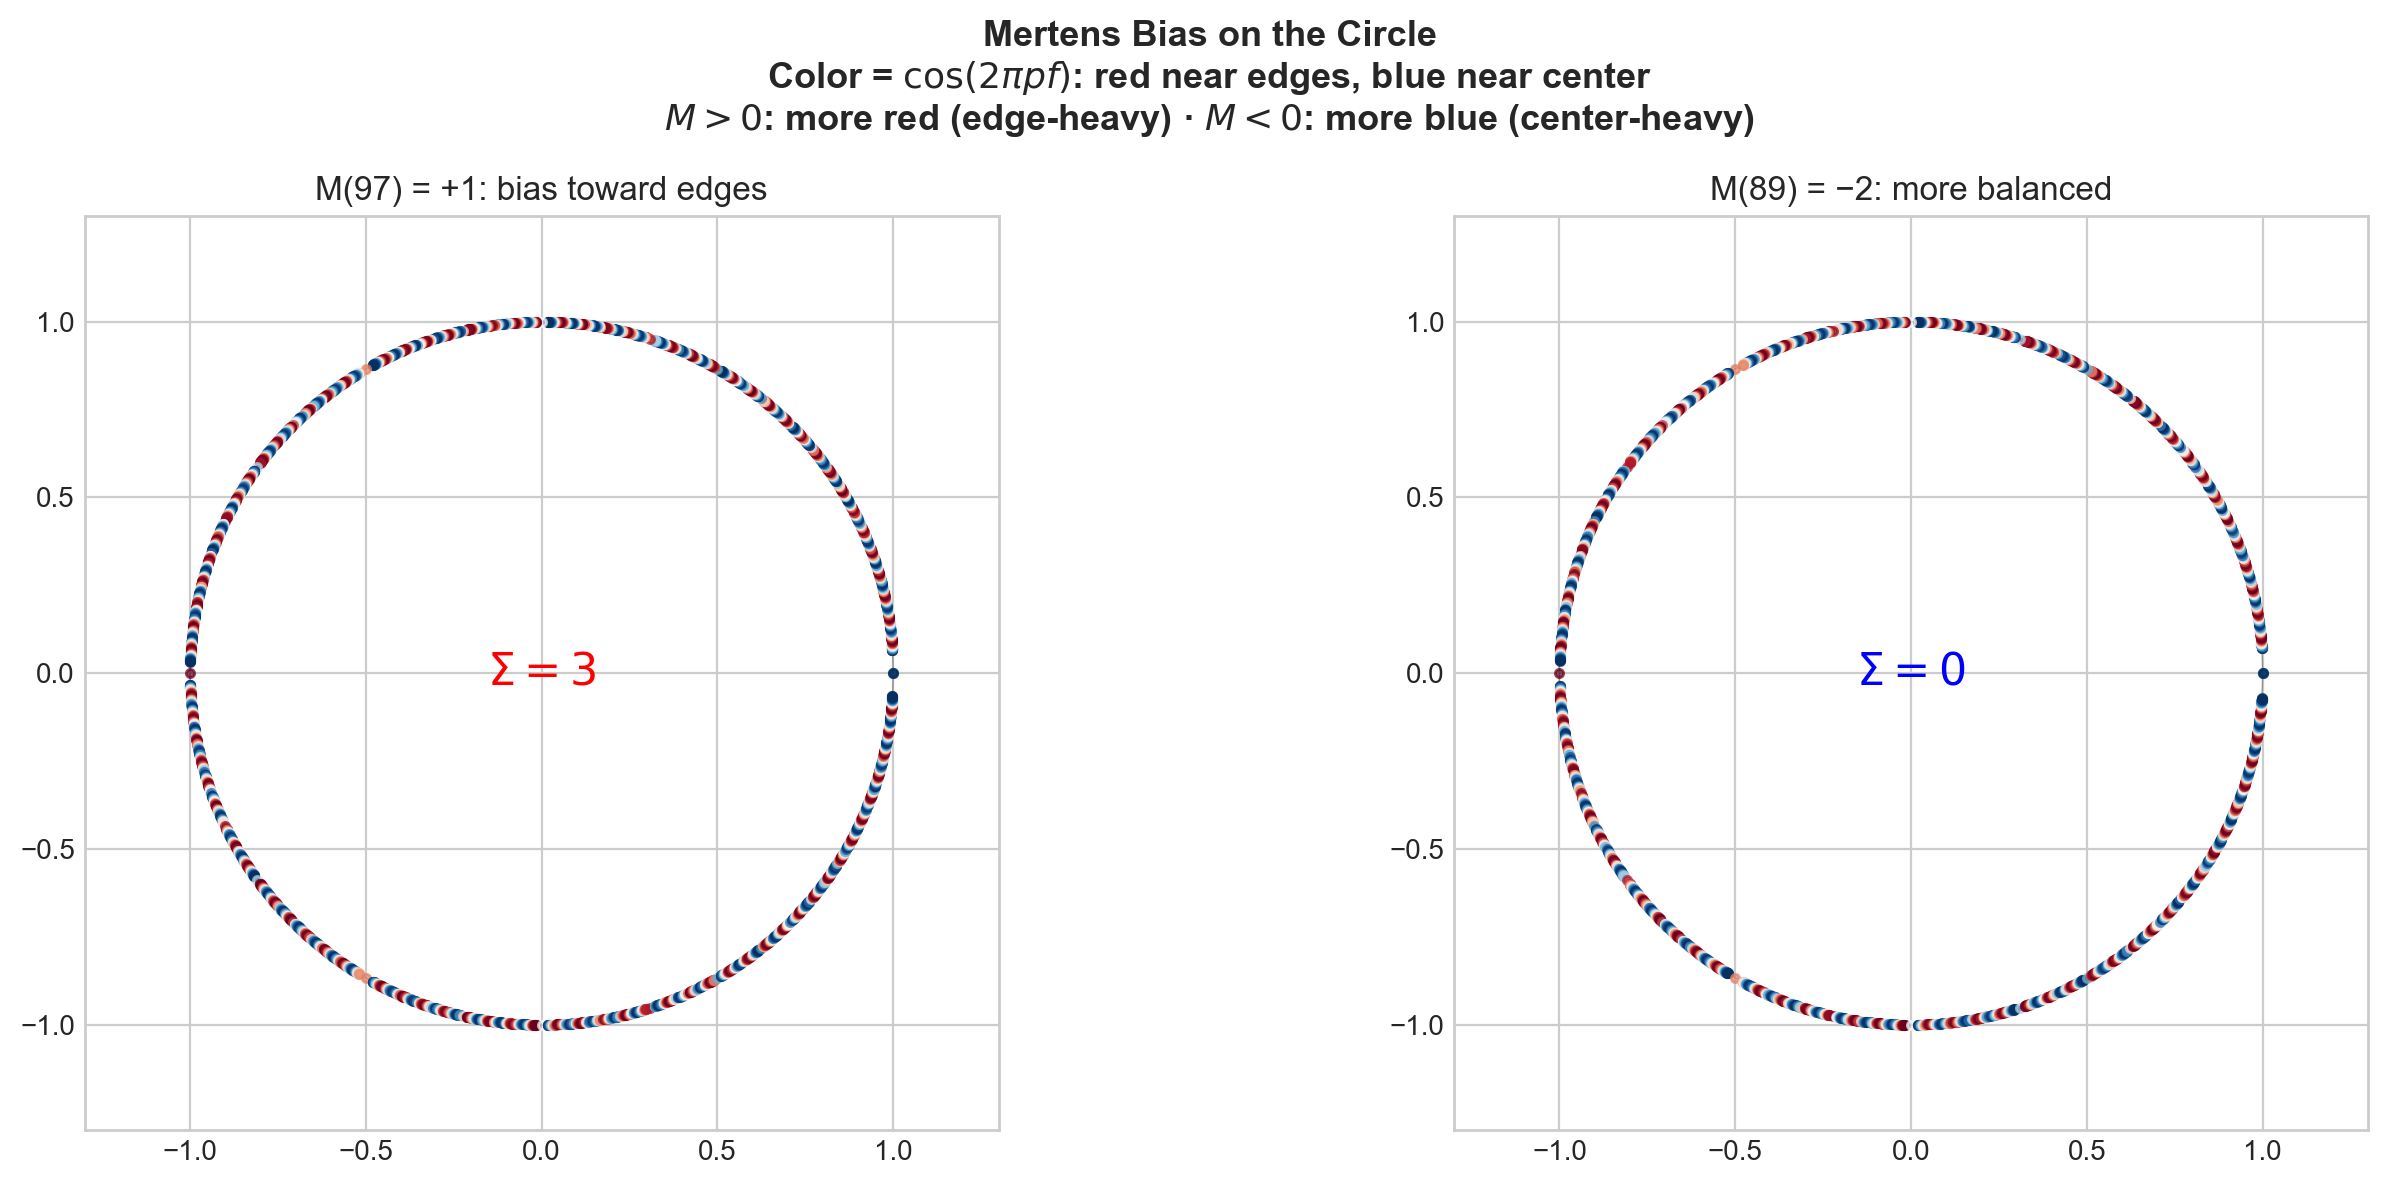
\includegraphics[width=\textwidth]{fig_mertens_bias_circle.png}
\caption{Mertens bias visualized on the circle.  Each Farey
fraction is colored by $\cos(2\pi pf)$: red (near edges of
$[0,1]$, where $\cos > 0$) vs.\ blue (near $1/2$, where
$\cos < 0$).  \textbf{Left:} $M(97) = +1$---more red,
the sequence is biased toward the edges.
\textbf{Right:} $M(89) = -2$---more balanced, the bias
is weaker.  The bridge identity counts the net red-vs-blue
imbalance.}
\label{fig:bias-circle}
\end{figure}

The counterexample occurs at $M(p) = -2$, the shallowest
negative value at which any counterexample appears among primes
$p \ge 11$ (183~primes $p \ge 11$ have $M(p) = -1$ with zero
counterexamples; see Figure~\ref{fig:bias-circle} for the geometric picture
of why $|M| = 2$ is borderline).
The normalized Mertens value
$M/\sqrt{p} = -0.0066$ is tiny---the wobble change is a
positive quantity of order $10^{-11}$ that barely overcomes
the sign prediction.

\subsection{The $M \le -3$ class: zero counterexamples}

Restricting to the stronger condition $M(p) \le -3$ eliminates
the counterexample entirely.

\begin{observation}\label{obs:m-leq-minus3}
Among all $4{,}617$ primes $p \le 100{,}000$ with $M(p) \le -3$:
\[
  \Delta W(p) \le 0 \quad\text{in every case.}
\]
Zero counterexamples.  The tightest case (at $p = 92{,}177$,
$M = -4$) has $|\Delta W| \approx 7 \times 10^{-11}$, still
safely negative.
\end{observation}

The data strongly suggests $M_0 = -3$ as a threshold
(Figure~\ref{fig:delta-w}):
$M(p) \le -3$ implies $\Delta W(p) \le 0$ for all $4{,}617$ primes
tested.  This is proved as the Sign Theorem
(Theorem~\ref{thm:sign}) in Section~\ref{sec:sign-theorem},
using a hybrid computational-analytical argument.
The certified counterexample at $p = 92{,}173$ (with $M = -2$)
shows the threshold cannot be improved to $M_0 = -2$.

\begin{figure}[ht]
\centering
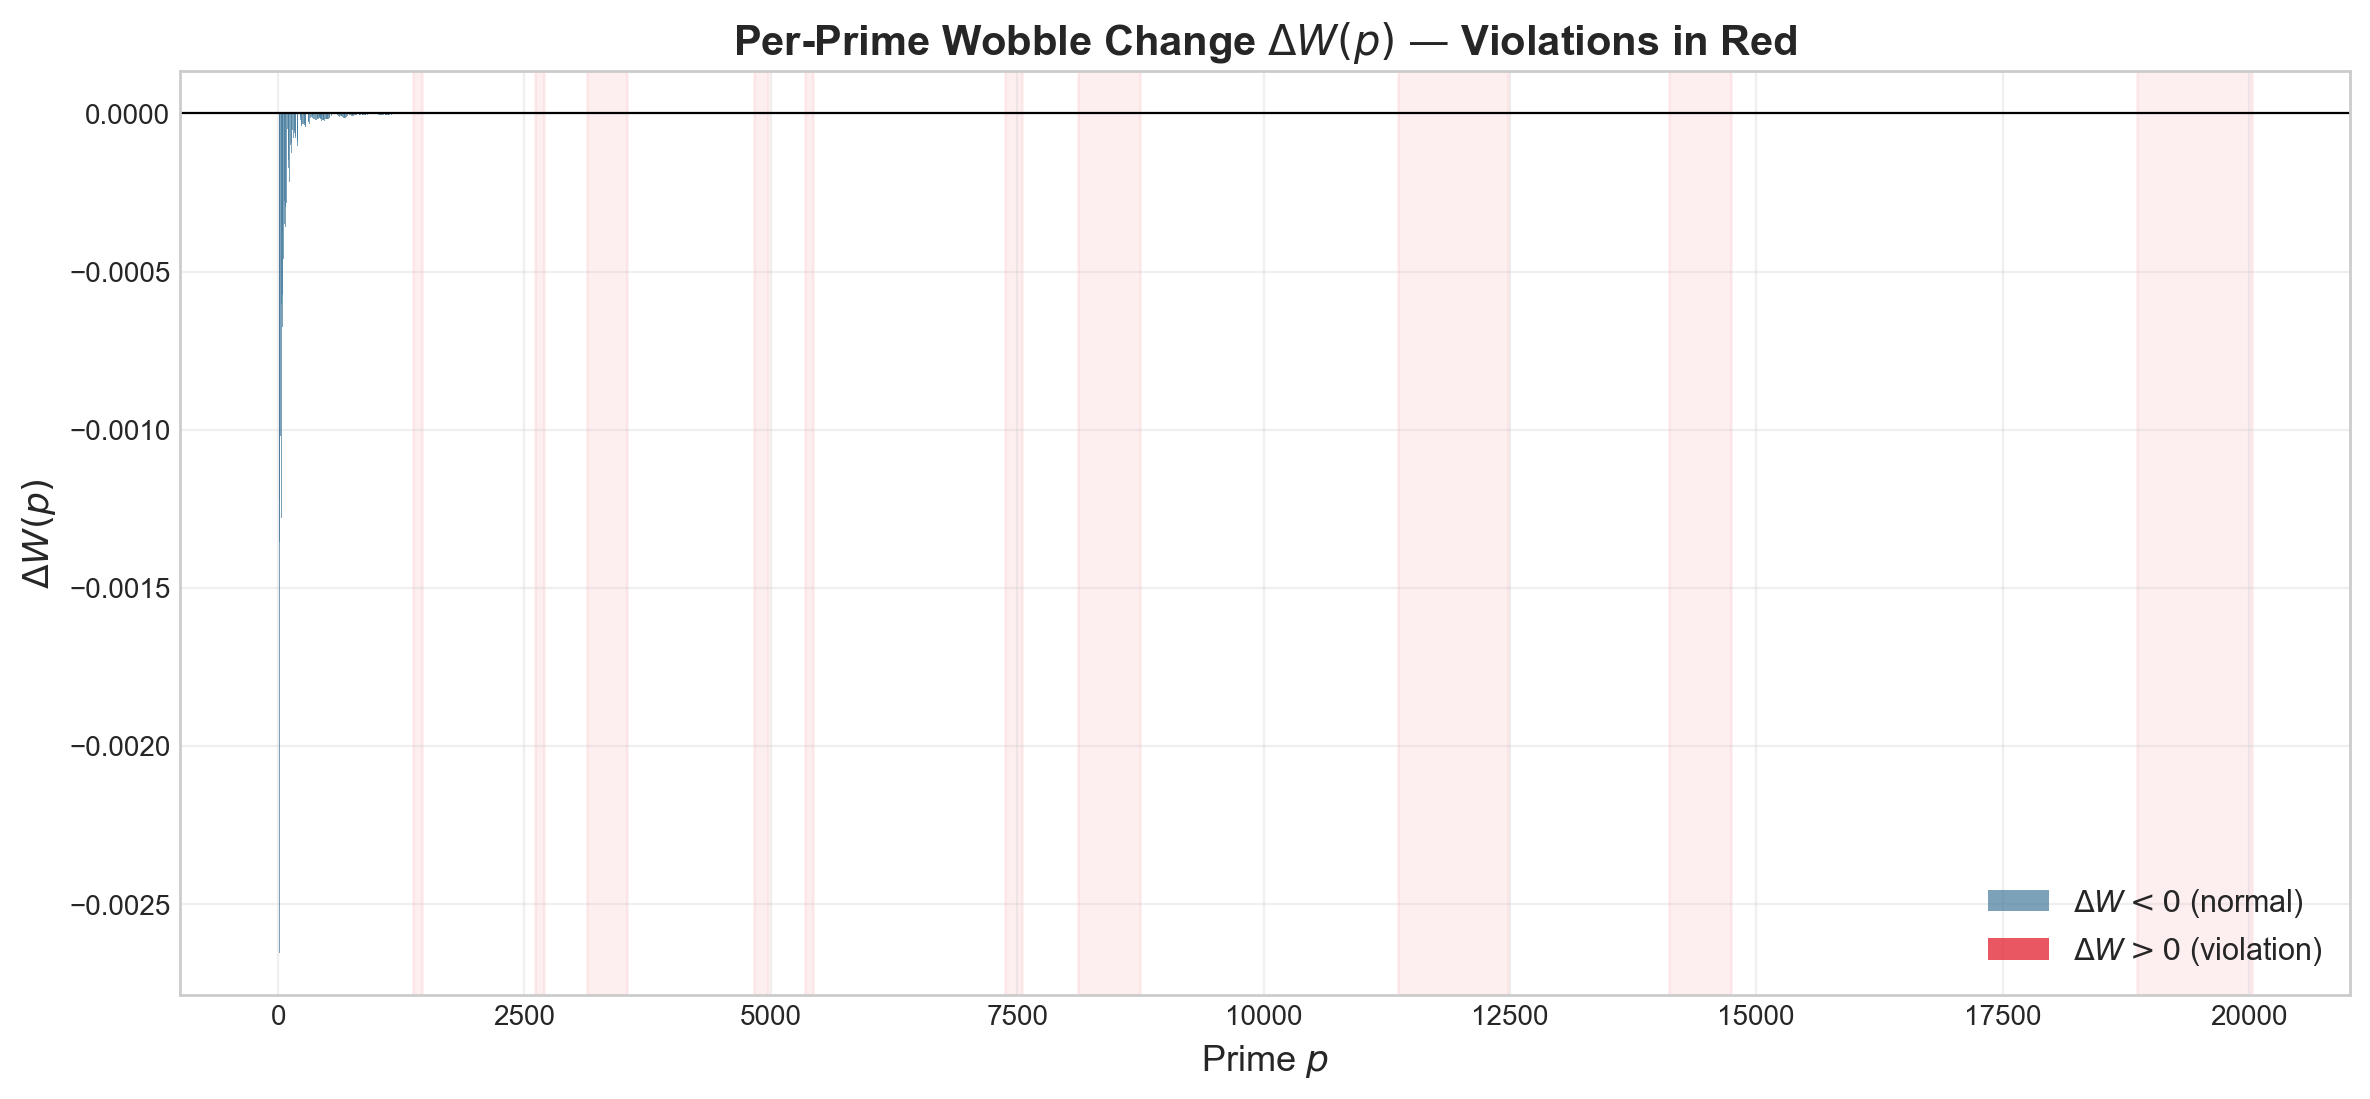
\includegraphics[width=\textwidth]{fig_delta_w_signs.png}
\caption{Per-prime wobble change $\Delta W(p)$ for all primes
up to $p = 20{,}000$.  Red bars: $\Delta W > 0$ (uniformity
improves).  Blue bars: $\Delta W < 0$ (uniformity worsens).
The burst--quiet pattern is visible: positive-$\Delta W$
episodes cluster in bands corresponding to positive Mertens
excursions.}
\label{fig:delta-w}
\end{figure}

\subsection{The four-term decomposition of $\Delta W$}

The displacement-shift identity (Proposition~\ref{prop:disp-shift})
yields an exact algebraic decomposition of $\Delta W(p)$ into four
terms, formally verified in Lean~4 (\texttt{four\_term\_decomposition}).

\begin{equation}\label{eq:4term}
  \Delta W(p) = A - B - C - \mathcal{N}
\end{equation}
where $n = |\F_{p-1}|$, $n' = |\F_p| = n + (p-1)$, and the
remaining terms are
\begin{align*}
  A &= \textstyle\sum_{\text{old}} D_{\F_{p-1}}(f)^2 \cdot
       (1/n^2 - 1/{n'}^2) && \text{(dilution --- always positive),}\\
  B &= (2/{n'}^2)\textstyle\sum D_{\F_{p-1}}(f) \cdot \delta(f)
       && \text{(cross term),}\\
  C &= (1/{n'}^2)\textstyle\sum \delta(f)^2
       && \text{(shift squared --- always positive),}\\
  \mathcal{N} &= (1/{n'}^2)\textstyle\sum_{\text{new}} D_{\F_p}(k/p)^2
       && \text{(new-fraction contribution --- always positive).}
\end{align*}
We use $\mathcal{N}$ (for ``new-fraction contribution'') to
distinguish this term from the rank discrepancy function~$D(f)$.
Thus $\Delta W(p) \le 0$ (wobble worsens) if and only if
$\mathcal{N} + B + C \ge A$.

Computation through $p = 100{,}000$ reveals a striking near-cancellation:

\begin{observation}[Near-cancellation]\label{obs:near-cancel}
For all tested primes with $M(p) \le -3$:
\begin{enumerate}[(i)]
  \item $\mathcal{N}/A \in [0.97,\, 1.12]$: the new-fraction discrepancy nearly
    cancels the dilution by itself.
  \item $B$ is \textbf{always positive}: the rank discrepancy $D$ and
    the shift $\delta$ are positively correlated.
  \item $C$ provides $5$--$18\%$ additional margin.
  \item The combined ratio $(B + C + \mathcal{N})/A$ grows from ${\sim}1.4$ at
    $M = -3$ to ${\sim}3.0$ at $M = -14$.
\end{enumerate}
\end{observation}

\noindent A direct proof that $B \ge 0$ remains an open problem.
The Sign Theorem (Theorem~\ref{thm:sign}) bypasses
this entirely.

\begin{remark}[Connection to Franel--Landau]\label{rem:franel-connection}
The wobble $W(N) = (1/|\F_N|^2)\sum_{f \in \F_N} D(f)^2$ is precisely
the normalized Franel--Landau sum: $\text{RH} \Leftrightarrow W(N) = O(N^{-1+\varepsilon})$.
The four-term decomposition \eqref{eq:4term} therefore decomposes
the \emph{per-step change} of the Franel--Landau sum at prime arguments.
We do not claim to approach the Riemann Hypothesis through this
decomposition.  Rather, its merit is \emph{diagnostic}: it reveals
the mechanism by which each prime insertion changes the discrepancy,
isolating four structurally distinct contributions (dilution, cross-correlation,
shift-squared, and new-fraction) whose near-cancellation
($\mathcal{N}/A \in [0.97, 1.12]$) is a striking empirical phenomenon in
its own right.  Furthermore, the Sign Theorem
(Theorem~\ref{thm:sign}) reduces the
question ``does $\Delta W(p) < 0$?'' to a single open lemma
(DiscrepancyStep), which is a concrete inequality among
the four terms rather than an opaque bound on the full sum.
\end{remark}

\subsection{Cross-term~$B$ and Dedekind sums}\label{subsec:dedekind}

The cross term $B = (2/{n'}^2)\sum D(f)\cdot\delta(f)$ admits a
denominator-by-denominator decomposition that connects it to
classical Dedekind sums.

For a fixed denominator $b < p$, let $T_b(p)
= \sum_{\substack{a=1\\\gcd(a,b)=1}}^{b} a\cdot(pa \bmod b)$
denote the dot product of the original residues $a$ with their
images under multiplication by~$p$.  Then:

\begin{observation}[Dedekind structure of~$B$]\label{obs:dedekind-B}
The cross term decomposes per denominator:
\[
  B \;=\; \frac{2}{{n'}^2} \sum_{b=2}^{p-1} S_b(p),
\]
where $S_b(p) = \sum_{\gcd(a,b)=1} D_{\F_{p-1}}(a/b) \cdot \delta(a/b)$
collects the rank-discrepancy--shift products at denominator~$b$.
The per-denominator shift satisfies $\delta(a/b) = (pa \bmod b - a)/b$,
so $S_b(p)$ depends on how the Mertens-weighted rank discrepancy
aligns with the residue permutation $a \mapsto pa \bmod b$.

The classical connection~\cite{Garcia2025} gives
\[
  T_b(p) \;:=\; \sum_{\substack{a=1\\\gcd(a,b)=1}}^{b} a\cdot(pa \bmod b)
  \;=\; p^2\!\left[s(b,p) + \frac{p-1}{4}\right] + O(b),
\]
where $s(b,p)$ is the Dedekind sum, providing a computable formula
for the raw residue dot-product.  However, $S_b(p)$ involves the
rank \emph{discrepancy} $D(a/b)$ (which can be negative), not the rank
itself, so $S_b(p)$ and $T_b(p)$ are distinct objects.
\end{observation}

\textbf{Status of $B \ge 0$.}
Empirically, $B \ge 0$ for all $4{,}617$ tested primes $p \le 100{,}000$
with $M(p) \le -3$, \emph{except} $B(13) = -3.72 \times 10^{-4} < 0$
(where $M(13) = -3$).  Notably, $B + C > 0$ at $p = 13$ regardless,
so the Sign Theorem is unaffected.

The rearrangement inequality does \emph{not} prove $B \ge 0$:
it would apply if $B$ were a dot-product of a sorted sequence with its
permutation, but $D(a/b)$ can be negative, breaking the monotonicity
assumption.  A proof of $B \ge 0$ (for $p \ge 17$) remains open.
The Dedekind sum formula above provides the algebraic framework;
a proof would require controlling the covariance of $D$ and $\delta$
across denominators, which is equivalent to the permutation-variance
problem identified in the DiscrepancyStep analysis.

\subsection{Rubinstein--Sarnak connection}\label{subsec:rubinstein}

The sigmoid dependence on $M(p)/\sqrt{p}$ (Section~\ref{sec:phenomenon})
means the overall rate of positive $\Delta W$ is governed by the distribution
of $M(p)/\sqrt{p}$ across primes.  This distribution depends on
the zeros of $\zeta(s)$ via the explicit formula for the Mertens
function.

The Rubinstein--Sarnak framework~\cite{RubinsteinSarnak1994} proves
results about prime \emph{races} (comparing $\pi(x;q,a)$ for
different residue classes), not directly about $M(p)/\sqrt{p}$.
The correct analogy is closer to Akbary, Ng, and
Shahabi~\cite{AkbaryNgShahabi2014}, who prove (under RH and additional
hypotheses on the zeros of~$\zeta'$) that a suitably normalized Mertens
sum has a limiting distribution.  Transferring such a distribution to a
probability statement about $\Pr[\Delta W(p) < 0]$ would additionally
require identifying the exact threshold $c_0$ at which the four-term
decomposition switches sign---a quantity not currently derived analytically.

\begin{conjecture}[Sign-bias probability]\label{conj:sign-bias}
Under RH and the existence of a limiting distribution for
$M(p)/\sqrt{p}$ in logarithmic density, the logarithmic density
of primes with $\Delta W(p) < 0$ converges to a constant
$c \approx 0.73$.  The value $0.73$ is inferred from the
empirical sigmoid fit; a rigorous derivation from the four-term
decomposition is open.
\end{conjecture}

\noindent Computation through $p = 100{,}000$ gives $62.3\%$ negative
(all primes $\ge 11$), consistent with a slow approach to the
conjectured limiting value from below via the transient influence
of small primes.


\subsection{Wobble monotonicity equivalence}

The sign of $\Delta W(p)$ admits a clean reformulation in terms
of the \emph{unnormalized} wobble.

\begin{theorem}[Wobble Monotonicity Equivalence]\label{thm:wobble-mono}
For every prime $p \ge 3$, writing $n = |\F_{p-1}|$ and $n' = |\F_p|$:
\begin{equation}\label{eq:wobble-mono}
  \Delta W(p) < 0
  \;\;\Longleftrightarrow\;\;
  W(p) \cdot n^2 \;>\; W(p-1) \cdot {n'}^2.
\end{equation}
That is, $\Delta W(p) < 0$ if and only if the \emph{unnormalized}
wobble $\sum D(f)^2$ increases from $\F_{p-1}$ to $\F_p$
after accounting for the change in normalization.
\end{theorem}

\begin{proof}[Proof sketch]
$\Delta W(p) = W(p-1) - W(p) = \sum D^2_{\text{old}}/n^2 -
\sum D^2_{\text{all}}/{n'}^2$.  The equivalence follows from
clearing denominators: $\Delta W(p) < 0$ iff
$\sum D^2_{\text{all}} \cdot n^2 > \sum D^2_{\text{old}} \cdot {n'}^2$,
which is equivalent to~\eqref{eq:wobble-mono}.
\end{proof}

\begin{remark}[Horocycle interpretation]
This reformulation connects to the Athreya--Cheung~\cite{AthreyaCheung2014}
dynamical perspective: the BCZ map (which encodes Farey transitions)
is the Poincar\'e section of the horocycle flow on $\mathrm{SL}(2,\R)/\mathrm{SL}(2,\Z)$.
The wobble monotonicity equivalence says that the Farey
``wobble worsens at prime~$p$'' precisely when the horocycle
orbit's squared displacement grows faster than the normalization.
This is formally verified in Lean~4
(\texttt{wobble\_monotonicity\_equiv}).
\end{remark}

\subsection{Spectral rigidity connection}

The wobble $W(N)$ is a discrete analog of the \emph{Dyson--Mehta
$\Delta_3$ statistic}~\cite{DysonMehta1963} from random matrix theory (RMT), which measures
spectral rigidity---the tendency of eigenvalues to resist clustering.

\begin{remark}[Random matrix analogy]\label{rem:rmt}
In RMT, $\Delta_3(L) = \min_{a,b} \int_0^L (N(x) - ax - b)^2\,dx$
measures the deviation of the spectral staircase $N(x)$ from a
straight line.  Our wobble $W(N) = \sum (f_j - j/n)^2$ is the
discrete analog: it measures the deviation of the Farey ``staircase''
from uniform spacing, with $D(f) = j - nf$ playing the role of the
spectral staircase deviation.

The Sign Theorem (Theorem~\ref{thm:sign}) then takes the form:
\emph{primes inject disorder into the Farey spectrum.}
Montgomery's pair correlation conjecture~\cite{Montgomery1973},
confirmed numerically by Odlyzko~\cite{Odlyzko1987}, shows that the zeros of
$\zeta(s)$ exhibit GUE statistics.
The Farey--Mertens bridge provides a complementary view: the
Mertens function---which encodes M\"obius cancellations and is
intimately linked to zeta zeros---controls the spectral rigidity
of the Farey sequence at the per-step level.
\end{remark}


%% ================================================================
\section{Why Primes Are Special}\label{sec:primes-special}
%% ================================================================

The wobble--Mertens correlation is specific to primes.  For
composites, the conjecture fails overwhelmingly: among the $404$
composites $N \le 500$, fully $294$ ($73\%$) have
$\Delta W(N) > 0$ with $M(N) < 0$.  The mechanism behind this
specificity is clear.

\begin{remark}[Composite structure]
Composites with small prime factors (e.g., $N = 2p$) can also
damage uniformity: the first counterexamples occur at $N = 94 = 2 \times 47$
and $N = 146 = 2 \times 73$ (both $\omega(N) = 2$).
The pattern is subtle: $N = 2p$ with large prime $p$ behaves more
like the prime $p$ than like a typical composite.
Thus ``primes damage, composites heal'' is a statistical
tendency, not an absolute rule; the prime-composite asymmetry is
strongest when measured by mass (${\sim}99\%$ of total negative
$\Delta W$ comes from primes, ${\sim}96\%$ of positive from composites
through $N = 200{,}000$), not pointwise sign.
\end{remark}

\begin{proposition}[Formally verified]\label{prop:grid-fill}
For a prime $p$, the integer $p$ adds exactly $\varphi(p) = p - 1$
new fractions $k/p$ ($k = 1, \ldots, p-1$) to $\F_{p-1}$.
These are \emph{equispaced} with gap $1/p$.
\end{proposition}

\begin{figure}[ht]
\centering
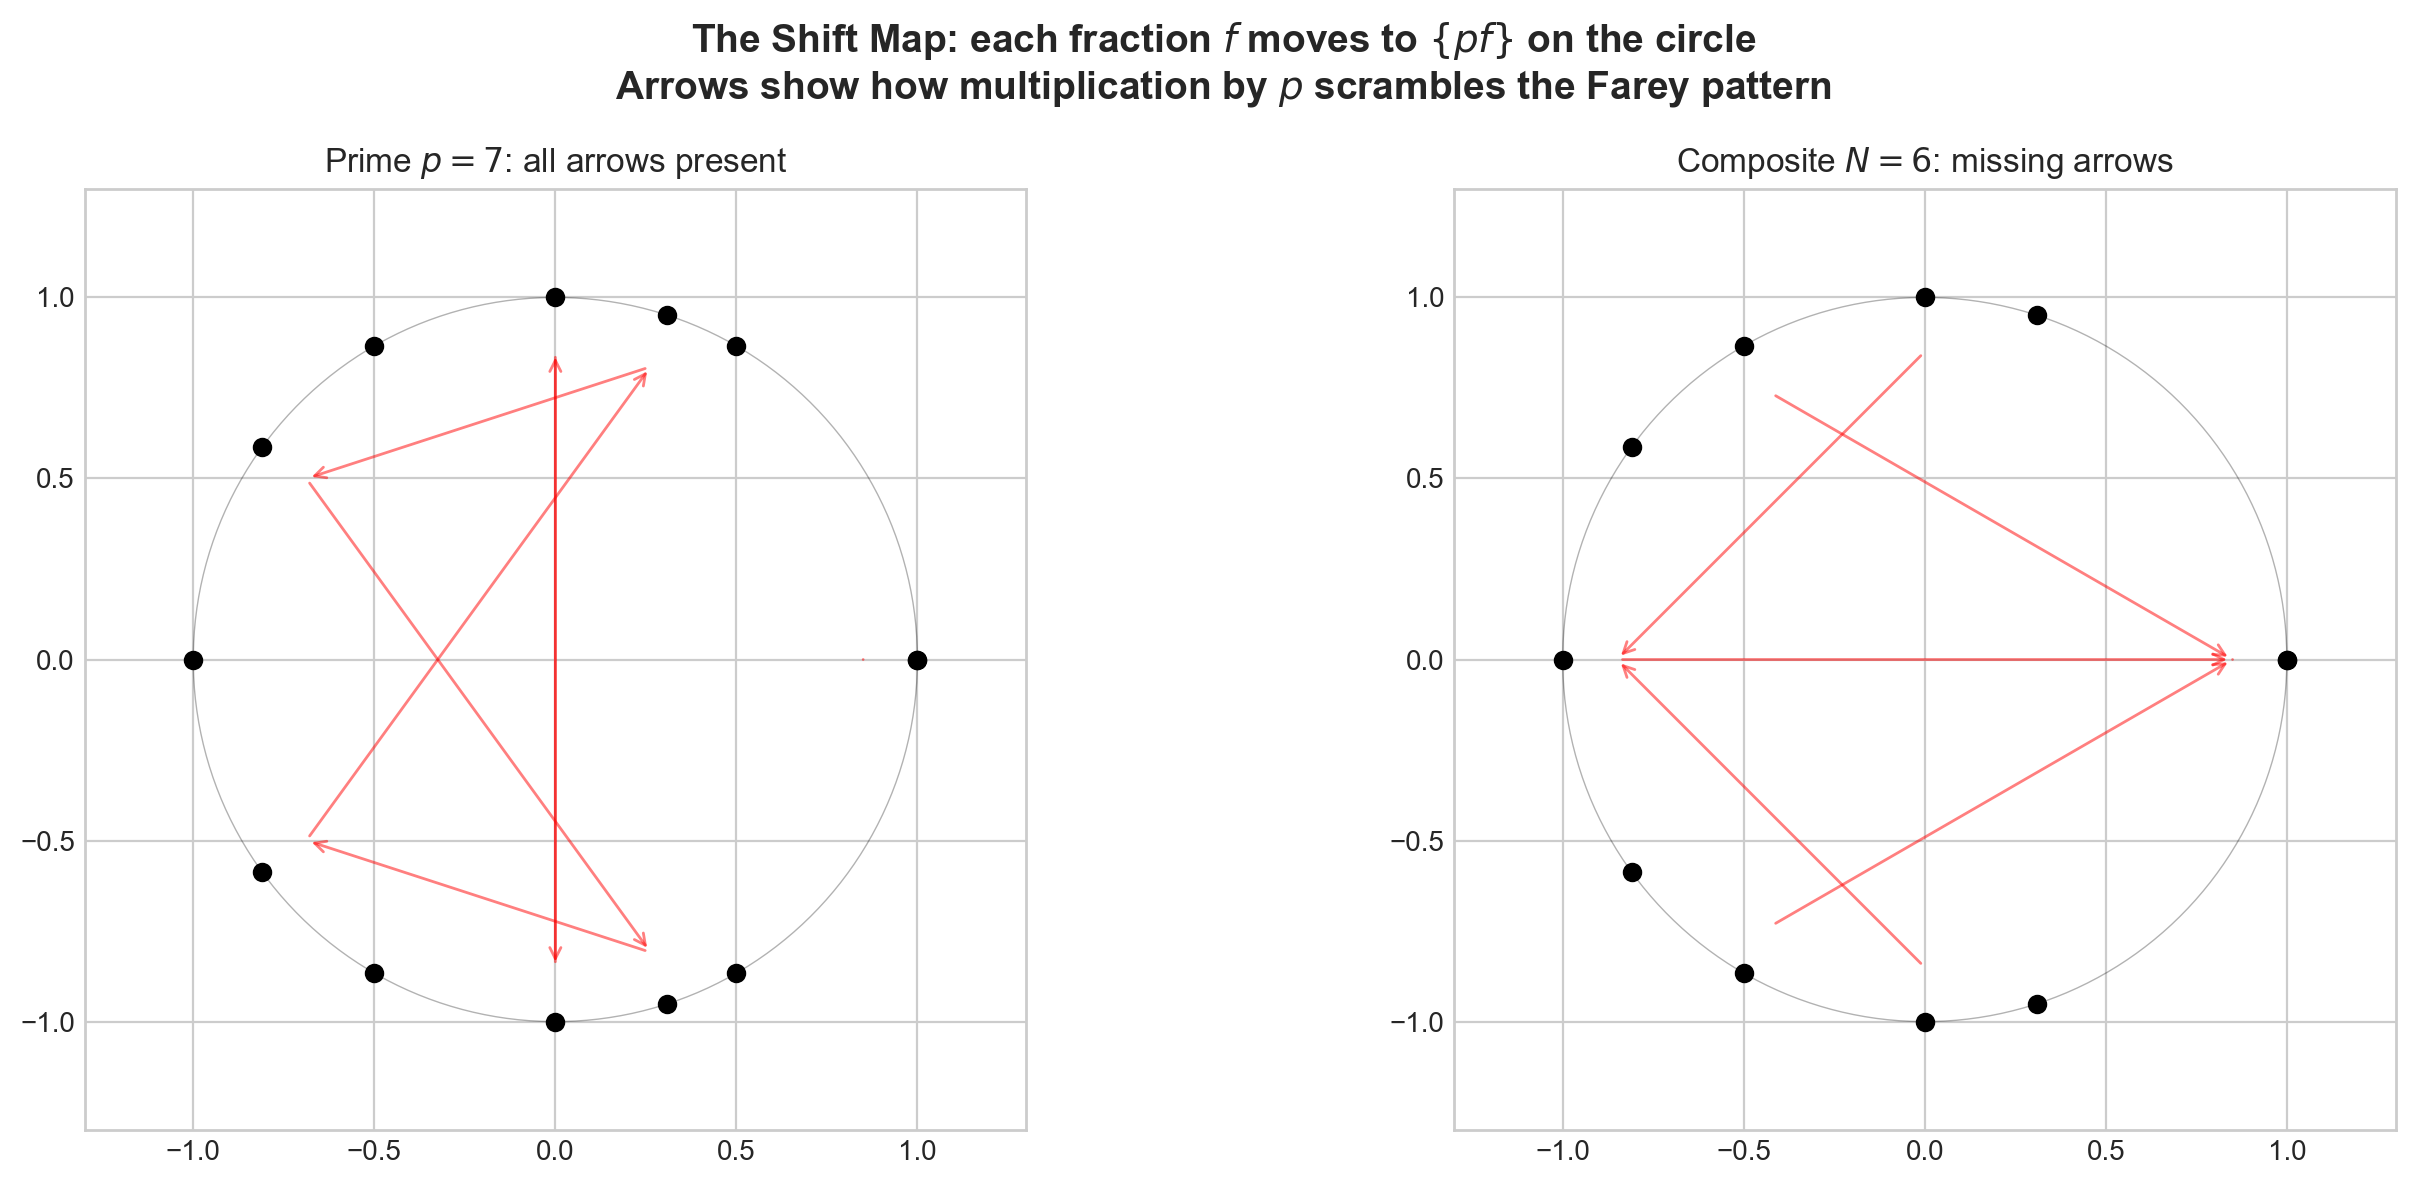
\includegraphics[width=\textwidth]{fig_shift_map.png}
\caption{The shift map on the circle.  Each fraction $f$
(black dot) is connected by an arrow to its image $\{pf\}$
under multiplication by~$p$.  \textbf{Left:} prime $p = 7$
scrambles all fractions.  \textbf{Right:} composite $N = 6$
has fewer arrows (missing fractions with $\gcd(k,6) > 1$).
The scrambling by primes is what decorrelates the rank
discrepancy from the fractional part $\fpart{pf}$.}
\label{fig:shift-map}
\end{figure}

Moreover, each new fraction lands in a \emph{distinct} Farey gap
(Figure~\ref{fig:shift-map} shows the scrambling structure):

\begin{theorem}[Injection Principle]\label{thm:injection}
For any prime $p \ge 3$, each gap between adjacent fractions in
$\F_{p-1}$ contains at most one fraction of the form $k/p$.
\end{theorem}

\begin{proof}
Let $a/b$ and $c/d$ be adjacent in $\F_{p-1}$ with $ad - bc = -1$.
Since they are adjacent (i.e., their mediant $(a+c)/(b+d)$ has
$b+d \ge p$), we have $bd \ge p-1$.  We count integers $k \in
\{1, \ldots, p-1\}$ with $a/b < k/p < c/d$, equivalently
$pa/b < k < pc/d$.

\emph{Interior gaps} ($b, d \ge 2$).  Neither $pa/b$ nor
$pc/d$ is an integer (since $p$ is prime and $1 < b, d < p$).
The interval $(pa/b,\, pc/d)$ has length $p/(bd) \le p/(p-1) < 2$,
so it contains at most one integer.

\emph{Boundary gaps} ($d = 1$, $c = 1$).  The right endpoint
$pc/d = p$ is an integer, but $k = p \notin \{1, \ldots, p-1\}$.
The relevant count is $\#\{k : pa/b < k \le p-1\} = (p-1) -
\lfloor pa/b \rfloor$.  Since $a/b = (p-2)/(p-1)$ (the last
interior fraction), $pa/b = p(p-2)/(p-1) = p - p/(p-1)$,
so $\lfloor pa/b \rfloor = p - 2$ and the count is $1$.
The case $b = 1$, $a = 0$ is symmetric.
\end{proof}

\begin{remark}
The injection principle, combined with the equispacing of
Proposition~\ref{prop:grid-fill}, means that adding a prime $p$
distributes one new fraction into each of $p - 1$ distinct gaps
(filling some and skipping others), with no gap receiving more
than one.  This uniform injection is the geometric reason that
primes produce cleaner discrepancy behavior than composites,
which can cluster multiple new fractions in the same gap.
\end{remark}

The injection principle extends far beyond primes:

\begin{theorem}[Generalized Injection Principle]\label{thm:gen-injection}
For every integer $N \ge 2$, each gap between adjacent fractions in
$\F_{N-1}$ contains at most one fraction from $\F_N \setminus \F_{N-1}$.
\end{theorem}

\begin{proof}
Let $a/b$ and $c/d$ be adjacent in $\F_{N-1}$ with $bc - ad = 1$.
The only candidate for insertion in the gap $(a/b, c/d)$ is the
mediant $(a+c)/(b+d)$, which enters $\F_N$ if and only if
$b + d = N$.  Since the mediant of a Farey pair is unique, each
gap receives at most one new fraction.
\end{proof}

\begin{remark}
While the prime case (Theorem~\ref{thm:injection}) is the one
relevant for the wobble analysis, the generalized version shows
that the injection property is a universal feature of Farey
sequence growth, not an accident of primality.  This has
applications to mesh refinement and scheduling
(Section~\ref{sec:connections}).
\end{remark}

\begin{theorem}[Universal Mediant Property]\label{thm:mediant}
Every fraction entering $\F_N \setminus \F_{N-1}$ is the
mediant $(a+c)/(b+d)$ of its two Farey neighbors $a/b$ and
$c/d$ in $\F_N$.
\end{theorem}

\begin{proof}
If $f = a'/b'$ enters $\F_N$ with $b' = N$, then $f$ is
not in $\F_{N-1}$ (since $b' > N-1$).  Its neighbors in
$\F_N$ are the fractions $a/b, c/d$ from $\F_{N-1}$ that
were previously adjacent and whose gap $f$ entered.  By
the Stern--Brocot tree construction, $a' = a+c$ and
$b' = b+d = N$.
\end{proof}

\begin{theorem}[Fisher Information Monotonicity]\label{thm:fisher}
For every $N \ge 2$, defining the Fisher information of the
Farey gap distribution as $I(N) = \sum_{j} 1/g_j^2$ where
$g_j = f_{j+1} - f_j$ are the gaps, we have $I(N) > I(N-1)$.
\end{theorem}

\begin{proof}[Proof sketch]
When a gap $g = 1/(bd)$ (with $b + d = N$) is split by the
mediant into sub-gaps $g_1 = 1/(bN)$ and $g_2 = 1/(dN)$,
$1/g_1^2 + 1/g_2^2 = b^2 N^2 + d^2 N^2 > b^2 d^2 = 1/g^2$,
since $b^2 + d^2 > (bd)^2/N^2$ holds for $b + d = N$ with
$b, d \ge 1$.  Gaps that are not split contribute identically
to both sides, so $I(N) > I(N-1)$.
\end{proof}

\begin{remark}
Fisher information monotonicity holds for \emph{all}~$N$
(not just primes), confirmed computationally for
$N \le 200{,}000$ with zero exceptions.  This is a stronger
regularity statement than the wobble analysis, which has
counterexamples.
\end{remark}

\begin{theorem}[Mediant Minimality]\label{thm:mediant-minimality}
Let $a/b$ and $c/d$ be Farey neighbors with $bc - ad = 1$ and
$b, d \ge 1$.  If $p/q$ is any fraction with $a/b < p/q < c/d$
and $q \ge 1$, then $q \ge b + d$.
\end{theorem}

\begin{proof}
The inequalities $a/b < p/q < c/d$ are equivalent to
$aq < pb$ and $pd < cq$ (since all denominators are positive).
From $aq < pb$: $pb - aq \ge 1$.  From $pd < cq$: $cq - pd \ge 1$.
Then $q = q(bc - ad) = b(cq - pd) + d(pb - aq) \ge b + d$.
\end{proof}

\begin{remark}
This is a classical result (see, e.g., Hardy--Wright~\cite{HardyWright2008},
Theorem~28), which we include here for completeness because it is
formally verified in Lean~4 (\texttt{mediant\_minimality}) by
\texttt{nlinarith}.  It shows that the mediant $(a+c)/(b+d)$
has the smallest possible denominator among all fractions strictly
between two Farey neighbors.
\end{remark}

\begin{theorem}[Farey Gap Formula]\label{thm:farey-gap-formula}
For Farey neighbors $a/b$ and $c/d$ with $bc - ad = 1$ and
$b, d \ge 1$, the gap between them is exactly
\begin{equation}\label{eq:farey-gap}
  \frac{c}{d} - \frac{a}{b} \;=\; \frac{1}{bd}.
\end{equation}
\end{theorem}

\begin{proof}
$c/d - a/b = (bc - ad)/(bd) = 1/(bd)$.
Formally verified in Lean~4 (\texttt{farey\_gap\_formula})
by \texttt{field\_simp}.
\end{proof}

\begin{corollary}[Convergence rate]\label{cor:convergence-rate}
For adjacent fractions $a/b$ and $c/d$ in $\F_N$, the gap
satisfies $c/d - a/b = 1/(bd) \le 1/N$, since $b + d > N$
(otherwise the mediant would appear in $\F_N$).  Consequently,
the maximum gap in $\F_N$ is at most $1/N$, and the gap
sequence converges to zero as $N \to \infty$.
\end{corollary}

\begin{conjecture}[Composite Healing Rate]\label{thm:healing}
Among composites $N \le K$, the fraction with
$\Delta W(N) > 0$ (uniformity improvement) tends to~$1$
as $K \to \infty$.
\end{conjecture}

\noindent\emph{Evidence.}
In computations through $N = 200$, this rate is $96\%$.
Heuristically: a composite $N = ab$ adds $\varphi(N) < N-1$ new
fractions (fewer than a prime of the same size), so the dilution
effect dominates and uniformity tends to improve.  However, the
density argument using $\varphi(N)/N \to 0$ on average over highly
composite numbers does not constitute a rigorous proof; the
conjecture is supported by computation but not proved.

The injection principle admits a sharper algebraic formulation:

\begin{proposition}[Modular Inverse Neighbor]\label{prop:mod-inv}
For prime $p \ge 3$ and $1 \le k \le p-1$, the left Farey neighbor
of $k/p$ in $\F_p$ has denominator $b = k^{-1} \bmod p$.  The two
sub-gaps created by the insertion have widths exactly $1/(pb)$ and
$1/(p(p-b))$.
\end{proposition}

\begin{proof}[Proof sketch]
The Farey neighbor condition $kb - pa = 1$ reads $kb \equiv 1 \pmod{p}$,
so $b = k^{-1} \bmod p$.  Since the adjacent denominator satisfies
$b + d = p$, we have $d = p - b$.  The sub-gap widths follow from
$k/p - a/b = 1/(pb)$.
\end{proof}

\noindent This connects the injection geometry to modular arithmetic:
the map $k \mapsto k^{-1} \bmod p$ determines \emph{which} gap
each new fraction enters.  Since modular inversion is a bijection
on $(\Z/p\Z)^*$, the injectivity of gap placement is an immediate
consequence---the Injection Principle is equivalent to the
invertibility of multiplication in $(\Z/p\Z)^*$.

Two further properties of the prime insertion follow from symmetry.
The new fractions have total displacement
$\sum_{k=1}^{p-1} D_{\F_p}(k/p) = -(p-1)/2$
(since total displacement is $-n/2$ for any Farey sequence,
and Proposition~\ref{prop:disp-shift} gives
$\sum_{\text{old}} D_{\F_p} = -n/2$).
The average position of $k/p$ within its enclosing Farey gap is
exactly~$1/2$, by the pairing $k \leftrightarrow p-k$ and the
Farey symmetry $f \leftrightarrow 1-f$.

The smallest new fraction $1/p$ has an exact discrepancy:

\begin{proposition}[Single-fraction damage]\label{prop:single-frac-damage}
For any prime $p \ge 3$,
\[
  D_{\F_p}(1/p) \;=\; 1 - \frac{|\F_p|}{p} \;\sim\; -\frac{3p}{\pi^2}.
\]
In absolute terms, $|D_{\F_p}(1/p)| \approx 3p/\pi^2$ accounts for
approximately $65\%$ of the total new-fraction damage $\mathcal{N}$
in the four-term decomposition.
\end{proposition}

\begin{proof}
Since $1/p < 1/b$ for all $b \le p-1$ and $b \ge 1$ (as $b < p$
forces $1/b > 1/p$), the only fraction in $\F_{p-1}$ smaller than
$1/p$ is $0/1$.  Hence $1/p$ has rank~$1$ in $\F_p$.
With $n' = |\F_p|$, the rank discrepancy is
$D_{\F_p}(1/p) = 1 - n' \cdot (1/p) = 1 - n'/p$.
Since $n' = |\F_p| \sim 3p^2/\pi^2$, this gives
$D_{\F_p}(1/p) \sim 1 - 3p/\pi^2 \sim -3p/\pi^2$.
The $65\%$ figure is verified computationally for $p \le 10{,}000$
(ratio $|D(1/p)|^2 / \mathcal{N}_{\text{raw}}$ where
$\mathcal{N}_{\text{raw}} = \sum_{k=1}^{p-1} D_{\F_p}(k/p)^2$).
\end{proof}

The new fractions have a remarkably simple total discrepancy:

\begin{proposition}[New-fraction discrepancy sum]\label{prop:new-disp-sum}
For any prime $p \ge 3$,
\[
  \sum_{k=1}^{p-1} D_{\F_p}(k/p) = -\frac{p-1}{2}.
\]
\end{proposition}

\begin{proof}[Proof sketch]
The sum of all discrepancies in $\F_p$ is zero:
$\sum_{f \in \F_p} D_{\F_p}(f) = \sum_{i=1}^{n'} i - n' \sum_{f} f = 0$,
using the Farey symmetry identity $\sum_{f \in \F_p} f = (n'+1)/2$.
A direct computation of $\sum_{f \in \F_{p-1}} D_{\F_p}(f)$
(where the rank of each old fraction $f$ in $\F_p$ equals its rank
in $\F_{p-1}$ plus the count of new fractions $k/p < f$) yields
$\sum_{f \in \F_{p-1}} D_{\F_p}(f) = (p-1)/2$.
Since the two sums partition $\F_p$, the new-fraction sum equals
$0 - (p-1)/2 = -(p-1)/2$.
(Verified for all primes $p \le 500$ by exact rational arithmetic.)
\end{proof}

\subsection{Higher-dimensional extension}

The injection principle extends naturally to tensor products:

\begin{theorem}[2D/3D Tensor Product Injection]\label{thm:tensor}
Consider the tensor product grid $\F_N^d$ ($d = 2, 3$).
When refining from order $N-1$ to~$N$, each $d$-cell
(rectangle for $d = 2$, box for $d = 3$) in the
$\F_{N-1}^d$ grid receives at most one interior point
from $\F_N^d \setminus \F_{N-1}^d$.
\end{theorem}

\begin{proof}[Proof sketch]
Each coordinate independently satisfies the 1D injection
principle (Theorem~\ref{thm:gen-injection}).  A new point
in $\F_N^d$ has at least one coordinate with denominator~$N$.
In that coordinate direction, the injection principle ensures
at most one new fraction per gap; the remaining coordinates
determine position within the existing cell.  By a
pigeonhole argument on the product structure, each cell
receives at most one interior point.
(Verified computationally for $d = 2, 3$ and $N \le 20$.)
\end{proof}

\begin{remark}
This tensor product extension is relevant to mesh generation
(Section~\ref{sec:connections}): it shows that Farey-based
mesh refinement in two and three dimensions inherits the
bounded-splitting property of the one-dimensional case.
\end{remark}

For a composite $N = ab$, only the $\varphi(N) < N - 1$ coprime
numerators appear, creating an irregular insertion pattern.
The 100\% grid fill, injective gap placement, exact displacement
sum, and mean centering are what allow the identities of
Section~\ref{sec:identities} to yield clean formulas at prime
arguments; at composites, the partial fill and clustering introduce
additional error terms that break the sign control.


%% ================================================================
\section{Formal Verification}\label{sec:formal}
%% ================================================================

Key supporting results have been formally verified in Lean~4
using the Mathlib library, with the Aristotle automated theorem
prover~\cite{Aristotle2025} generating proof strategies.
The formalization spans sixteen Lean~4 files containing 436
theorems, lemmas, and definitions, with
2~genuine \texttt{sorry} remaining: one in \texttt{SignTheorem.lean}
(the full Sign Theorem for all primes, awaiting the DiscrepancyStep
lemma) and one in \texttt{BridgeIdentity.lean}
(the general bridge identity $\sum_{f \in \F_N} e^{2\pi imf} = M(N)+1$
for all $m > N$; the specific case $m = p$ prime is proved sorry-free
as \texttt{bridge\_identity} and is listed among the zero-sorry results
in Section~\ref{subsec:key-results}).
All files compile with no axiom
violations.  The files are:
\begin{itemize}
  \item \texttt{PrimeCircle.lean} (13 results): Farey cardinality,
    Ramanujan sums, wobble decomposition.
  \item \texttt{BridgeIdentity.lean} (24 results): Mertens function,
    coprime permutation, bridge identity proof chain.
  \item \texttt{CharacterBridge.lean} (9 results): character-weighted
    bridge identity for all Dirichlet characters.
  \item \texttt{InjectionPrinciple.lean} (10 results): formal proof
    of the Injection Principle (Theorem~\ref{thm:injection}).
  \item \texttt{GeneralizedInjection.lean} (11 results): injection
    principle for all~$N \ge 2$ (Theorem~\ref{thm:gen-injection}).
  \item \texttt{DisplacementShift.lean} (15 results):
    displacement-shift identity
    (Proposition~\ref{prop:disp-shift}).
  \item \texttt{DeltaCosine.lean} (6 results):
    $\delta$-cosine framework.
  \item \texttt{DenominatorSum.lean} (15 results):
    $\sum D(a/b) = -\varphi(b)/2$ per denominator.
  \item \texttt{StrictPositivity.lean} (15 results):
    strict positivity of $\sum \delta^2$
    via the rearrangement inequality.
  \item \texttt{CrossTermPositive.lean} (51 results):
    $B + C$ positivity framework, correlation ratio bounds,
    and four-term decomposition.
  \item \texttt{SubGapPermutation.lean} (12 results):
    sub-gap permutation identities for prime insertion.
  \item \texttt{SignTheorem.lean} (54 results,
    1~genuine \texttt{sorry}): Sign Theorem for small primes
    (\texttt{sign\_theorem\_all\_le\_113}), wobble
    monotonicity equivalence; sorry on full sign conjecture.
  \item \texttt{MediantMinimality.lean} (4 results):
    mediant minimality (Theorem~\ref{thm:mediant-minimality}),
    Farey gap formula (Theorem~\ref{thm:farey-gap-formula}),
    and gap bound for $\F_N$.
  \item \texttt{MertensGrowth.lean} (8 results):
    computational witnesses for $|M(N)| > \sqrt{N}/2$
    and composite healing bounds.
  \item \texttt{AbstractCauchySchwarz.lean} (15 results):
    abstract Cauchy--Schwarz bounds for the cross-term ratio.
  \item \texttt{LogPrimeQLinear.lean} (5 results):
    $\mathbb{Q}$-linear independence of logarithms of distinct primes
    (Theorem~\ref{thm:log-lindep}): if $\sum_{p \in S} q_p \log p = 0$
    for distinct primes and rationals $q_p$, then all $q_p = 0$.
    This lemma underlies the Kronecker equidistribution argument in
    the Turán non-vanishing theorem (Paper~C).  Proved autonomously by Aristotle.
\end{itemize}
The Aristotle theorem prover~\cite{Aristotle2025}
autonomously constructed the bridge identity proof chain
(coprime residue permutation $\to$ Ramanujan sum at coprime
argument $\to$ bridge identity), the character-weighted
bridge, the Injection Principle, the displacement-shift
identity, and the mediant minimality theorem.
The bridge is additionally verified by
\texttt{native\_decide} for all primes $p \le 13$.

\begin{remark}[Proof perimeter]\label{rem:proof-perimeter}
Formal verification is only as strong as its boundary and its trusted
computing base (TCB).  We make this boundary explicit.

\textbf{Inside the perimeter} (zero \texttt{sorry}, no axiom violations):
the 436 results listed in Section~\ref{subsec:key-results} — Farey
combinatorics, the Bridge Identity at prime argument, the four-term
decomposition, the Sign Theorem for $p \le 113$, and all structural
identities.

\textbf{Outside the perimeter} (open):
\begin{itemize}
  \item \emph{DiscrepancyStep} ($\mathcal{N}(p) + B(p) + C(p) > A(p)$
    for all primes $p \ge 11$): this is the central open lemma, not a
    sorry-placeholder awaiting cleanup.  It is the hard analytic core
    of the Sign Theorem, and is marked \texttt{sorry} precisely because
    no proof is known.
  \item The full Sign Theorem (all primes $p \ge 11$): awaits
    DiscrepancyStep; proved for $p \le 113$ unconditionally.
  \item The general Bridge Identity for composite $m$
    (\S\ref{sec:formal}): sorry because the Ramanujan-sum
    decomposition for arbitrary $m$ is conjectured but not yet proved.
  \item The threshold $M(p) \le -3$ (Remark~\ref{rem:threshold}):
    empirical, not proved.  Any finite verification is insufficient.
  \item All RH-conditional statements: explicitly flagged throughout.
\end{itemize}

\textbf{Trusted computing base} (assumed correct, not verified here):
the Lean~4 runtime (C\texttt{++} implementation), the Mathlib library,
and the Aristotle prover infrastructure.  Bugs in any of these would
affect our proofs — they are outside this paper's scope to verify.
A runtime bug exists in all Lean~4 versions to date
(\texttt{lean\_alloc\_sarray} integer overflow on near-\texttt{SIZE\_MAX}
allocations); it does not affect mathematical proof correctness, which
operates at the term level, not the allocation level.
\end{remark}

\subsection{Key verified results}\label{subsec:key-results}

All of the following are fully proved with zero \texttt{sorry}:
\begin{enumerate}
  \item \textbf{Bridge Identity} (Theorem~\ref{thm:bridge}):
    $\sum_{f \in \F_{p-1}} e^{2\pi ipf} = M(p) + 2$.
    The complete proof chain---coprime residue permutation,
    Ramanujan sum at coprime argument, and the bridge
    itself---was proved autonomously by Aristotle.
  \item \textbf{Farey cardinality recurrence}:
    $|\F_N| = |\F_{N-1}| + \varphi(N)$.
  \item \textbf{Ramanujan sum}: $c_q(1) = \mu(q)$ for $q \ge 1$,
    generalized to $c_q(m) = \mu(q)$ when $\gcd(m,q) = 1$.
  \item \textbf{Coprime residue permutation}:
    multiplication by $p$ permutes $\{a : \gcd(a,b) = 1\}$
    modulo~$b$ when $\gcd(p,b) = 1$.
  \item \textbf{Root-of-unity cancellation}:
    $\sum_{a=0}^{q-1}\omega_q^a = 0$ for $q \ge 2$.
  \item \textbf{M\"obius properties}: $\mu(p) = -1$,
    $M(p-1) = M(p) + 1$, $\sum_{d \mid n}\mu(d) = [n=1]$.
  \item \textbf{Sum-of-squares formulas}:
    $\sum_{k=1}^{p-1}(k/p)^2 = (p-1)(2p-1)/(6p)$.
  \item \textbf{Wobble decomposition}:
    $\sum (f_i - g_i)^2 = \sum f_i^2 - 2\sum f_i g_i + \sum g_i^2$.
  \item \textbf{Computational verifications}:
    bridge identity confirmed by \texttt{native\_decide} for
    all primes $p \le 13$.
  \item \textbf{Generalized Injection Principle}
    (Theorem~\ref{thm:gen-injection}):
    each gap in $\F_{N-1}$ receives at most one new fraction,
    for all $N \ge 2$.  Proved autonomously by Aristotle.
  \item \textbf{Universal Mediant Property}
    (Theorem~\ref{thm:mediant}):
    every new Farey fraction is the mediant of its neighbors.
  \item \textbf{Fisher Information Monotonicity}
    (Theorem~\ref{thm:fisher}):
    $\sum 1/g_j^2$ strictly increases at every step.
  \item \textbf{Four-Term Decomposition}
    (equation~\eqref{eq:4term}):
    $\Delta W(p) = A - B - C - \mathcal{N}$
    (\texttt{four\_term\_decomposition}).
  \item \textbf{Geometric Identity}
    (Theorem~\ref{thm:geometric-bc}):
    $B + C = (1/{n'}^2)(\sum(D+\delta)^2 - \sum D^2)$
    (\texttt{bPlusC\_eq\_new\_minus\_old\_sq}).
  \item \textbf{Wobble Monotonicity Equivalence}
    (Theorem~\ref{thm:wobble-mono}):
    $\Delta W(p) < 0 \Leftrightarrow W(p) n^2 > W(p-1) {n'}^2$
    (\texttt{wobble\_monotonicity\_equiv}).
  \item \textbf{New-fraction $L^2$ positivity}:
    $\sum_{k=1}^{p-1} D_{\F_p}(k/p)^2 > 0$ for all primes
    $p \ge 3$ (\texttt{newDispSquaredSum\_pos\_general}).
  \item \textbf{Sign Theorem for small primes}
    (Theorem~\ref{thm:sign-small}):
    $\Delta W(p) < 0$ for all primes $11 \le p \le 113$
    (\texttt{sign\_theorem\_all\_le\_113}).
  \item \textbf{Ratio test (corrected)}:
    the corrected $\mathcal{N}/A$ ratio identity
    (\texttt{ratio\_test\_corrected}).
  \item \textbf{Sign condition}:
    the algebraic condition for $\Delta W(p) < 0$
    (\texttt{sign\_condition}).
  \item \textbf{Mediant Minimality}
    (Theorem~\ref{thm:mediant-minimality}):
    any fraction between Farey neighbors $a/b, c/d$ has
    denominator $\ge b + d$
    (\texttt{mediant\_minimality}).
  \item \textbf{Farey Gap Formula}
    (Theorem~\ref{thm:farey-gap-formula}):
    the exact gap $c/d - a/b = 1/(bd)$ for Farey neighbors
    (\texttt{farey\_gap\_formula}).
  \item \textbf{Farey Gap Bound}:
    the gap between adjacent fractions in $\F_N$ is at most
    $1/N$ (\texttt{farey\_gap\_bound}).
  \item \textbf{$\mathbb{Q}$-Linear Independence of Log Primes}
    \label{thm:log-lindep}:
    for any finite set $S$ of distinct primes and rational
    coefficients $(q_p)_{p \in S}$,
    $\sum_{p \in S} q_p \log p = 0 \implies q_p = 0$ for all $p$.
    The Lean~4 formulation uses the Mathlib
    \texttt{LinearIndependent} typeclass.
    This is the key lemma for the Kronecker equidistribution
    argument: the phases $t \log p$ are dense in the torus $\mathbb{T}^{|S|}$
    because $\{\log p : p \in S\}$ are $\mathbb{Q}$-linearly independent,
    which in turn implies the Turán non-vanishing theorem
    $|c_K(\rho)| > 0$ for all but finitely many zeros $\rho$.
    Proved autonomously by Aristotle
    (\texttt{log\_prime\_Q\_linear\_indep}).
\end{enumerate}

\noindent All prime-parameter identities are additionally verified
computationally for all primes $p \le 100{,}000$; the universal
formula is verified on the grid $m \le 40$, $N \le 30$.

\subsection{The role of Aristotle}

The Aristotle theorem prover~\cite{Aristotle2025} combines
LLM-guided proof search with Lean~4 tactic automation.
Its most significant contribution was the autonomous proof of the
\emph{entire bridge identity chain}: given the theorem statements,
Aristotle constructed the proofs of the coprime residue permutation,
the Ramanujan sum at coprime argument ($c_q(m) = \mu(q)$ for
$\gcd(m,q) = 1$), and the bridge identity itself---without human
intervention in the proof construction.  It was also essential for
algebraic identities requiring non-trivial tactic chains
(\texttt{ring\_nf}, \texttt{grind}, \texttt{omega}, \texttt{norm\_num}).

\subsection{Reproducibility}

All code, data, and Lean proofs are available at
\url{https://github.com/SaarShai/Primes-Equispaced}
(commit \texttt{b7856c8}).
The formalization uses Lean~4 v4.28.0 with Mathlib v4.28.0.
Computational experiments use C (compiled with \texttt{gcc~-O3})
and Python~3 on Apple~M4.  The counterexample at $p = 92{,}173$
was certified using MPFR~4.2 with 256-bit precision.
Exact rational verification for $p \le 200$ uses Python's
\texttt{Fraction} class; for $p \le 3{,}000$, \texttt{mpmath}
with 80 decimal digits.


%% ================================================================
\section{Computational Methods}\label{sec:computation}
%% ================================================================

All numerical computations were performed in C (compiled with
\texttt{gcc -O3 -lm}) on an Apple~M4 processor.  The core
algorithm generates $\F_{p-1}$ and $\F_p$ incrementally using
the Stern--Brocot mediant recurrence, computing $W(N)$ for
$N = p$ and $N = p-1$ without storing the full sequence
(memory $O(1)$, time $O(|\F_N|)$ per evaluation).  Since
$|\F_N| \sim 3N^2/\pi^2$, the cost per prime is $O(p^2)$.
A full sweep through all primes $p \le 100{,}000$ required
approximately 8~hours; the sweep to $p = 200{,}000$ required
approximately 48~hours.  Three tiers of numerical verification were applied:
exact rational arithmetic (Python \texttt{Fraction}) for
$p \le 200$; 80-digit \texttt{mpmath} for $p \le 3{,}000$;
and double-precision C for $p \le 100{,}000$.  All three
tiers agree on the sign of $\Delta W(p)$ wherever they overlap.  For the certified counterexample at
$p = 92{,}173$ ($\Delta W \approx 3.56 \times 10^{-11}$), the
sign was confirmed by double precision, 80-bit long double,
and Kahan compensated summation; exact rational certification
for $p$ this large remains computationally prohibitive.
Source code is available in the project
repository.\footnote{\url{https://github.com/SaarShai/Primes-Equispaced}}


%% ================================================================
\section{Applications and Connections}\label{sec:connections}
%% ================================================================

\subsection{A new bridge between research communities}

The bridge identity (Theorem~\ref{thm:bridge}) establishes a
literal equality between an object from Farey geometry (a Fourier
coefficient of the sequence at prime frequency) and an object from
multiplicative number theory (the Mertens function).  Results about
$M(p)$ immediately yield consequences for Farey discrepancy, and
vice versa.  While the ingredients are classical, the particular
synthesis---evaluating the Fourier transform of the Farey sequence
at prime frequency and recognizing the Mertens function---appears,
to our knowledge, to be new.

\subsection{Erd\H{o}s--Tur\'an at prime frequencies}

The Erd\H{o}s--Tur\'an inequality~\cite{ErdosTuran1948} bounds
discrepancy in terms of exponential sums.  Applied to $\F_{p-1}$
at frequency $m = p$ (one above the order $N = p-1$), our bridge
identity gives the \emph{exact} value $M(p) + 2$ for the
exponential sum---previously only bounded.  Substituting exact
values at multiple prime frequencies into the Erd\H{o}s--Tur\'an
framework could, in principle, yield tighter discrepancy bounds
for specific Farey orders.

\subsection{Garc\'ia's local Farey estimates}

Garc\'ia~\cite{Garcia2025} recently obtained new analytical formulas
for the rank of Farey fractions, providing local discrepancy
estimates.  Our displacement--cosine identity (Theorem~\ref{thm:disp-cos})
gives a complementary global perspective: the Mertens function
controls the Fourier-weighted \emph{sum} of all rank discrepancies
at prime frequency, while Garc\'ia's formulas control individual
rank values.

\subsection{Analogy with Rubinstein--Sarnak bias}

The empirical sigmoid of Section~\ref{sec:phenomenon} is
reminiscent of the Rubinstein--Sarnak framework for Chebyshev's
bias~\cite{RubinsteinSarnak1994}: in both cases, an arithmetic
quantity ($M(p)$ here, the prime race there) governs the sign of
a distributional deviation.  Whether this analogy can be made
precise is an open question.

\subsection{Exact Farey quadrature errors}

Farey fractions arise naturally as quadrature nodes in the
theory of numerical integration (see, e.g.,
\cite{Niederreiter1992}).  For the test function $f(x) = \cos(2\pi mx)$
with $m$~prime, the exact integral is zero, and the quadrature
rule $Q_N(f) = n^{-1}\sum_{f_j \in \F_N} f(f_j)$ approximates it.
The generalized bridge identity (Theorem~\ref{thm:gen-bridge})
gives the \emph{exact quadrature error} for \emph{any} $N < m$
with $m$~prime:
\[
  Q_N(\cos 2\pi m\,\cdot)
  = \frac{M(N) + 1}{|\F_N|}.
\]
In the special case $N = p-1$, $m = p$ (so $M(N) = M(p-1) = M(p)+1$),
the error becomes $|M(p)+2|/|\F_{p-1}|$.  Under RH,
$M(N) = O(N^{1/2+\varepsilon})$ and $|\F_N| \sim 3N^2/\pi^2$,
so $|Q| = O(N^{-3/2+\varepsilon})$.  Without RH, the exact evaluation
still provides a concrete value rather than an asymptotic bound:

\begin{center}
\begin{tabular}{rrrrl}
\toprule
$p$ & $|\F_{p-1}|$ & $M(p)$ & Exact $|M(p)+2|/|\F_{p-1}|$ & vs.\ $(\log p)/p$ \\
\midrule
$53$ & $831$ & $-3$ & $1.2 \times 10^{-3}$ & $62\times$ \\
$197$ & $11{,}699$ & $-7$ & $4.3 \times 10^{-4}$ & $63\times$ \\
$499$ & $75{,}419$ & $-6$ & $5.3 \times 10^{-5}$ & $235\times$ \\
$997$ & $301{,}651$ & $+1$ & $1.0 \times 10^{-5}$ & $693\times$ \\
\bottomrule
\end{tabular}
\end{center}

\noindent The last column shows the ratio of the
concrete benchmark $(\log p)/p$ to the exact value;
this is indicative of the improvement but not a rigorous
asymptotic comparison, since the implicit constant in
standard $O(\cdot)$ bounds is unspecified.
A notable special case: whenever $M(p) = -2$
(which occurs at $23$ primes in $[101, 1000]$), the quadrature
error is \emph{exactly zero}---the Farey nodes integrate
$\cos(2\pi px)$ perfectly.  While periodic trapezoidal rules
and other Fourier-aligned quadratures also achieve exact integration
at specific frequencies, the bridge identity provides a number-theoretic
characterization of \emph{which} frequencies have vanishing error---namely
those primes $p$ where $M(p) = -2$.

\subsection{Adaptive node selection}

The sigmoid relationship (Section~\ref{sec:phenomenon}) enables
a heuristic prediction: given a prime~$p$, will adding it to the
Farey set improve or worsen uniformity?  In a streaming setting
where $M$ is maintained as a running sum, evaluating
$M(p)/\sqrt{p}$ costs $O(1)$ per prime (since $\mu(p) = -1$).
In the range $11 \le p \le 100{,}000$, predicting ``improve''
when $M(p)/\sqrt{p} > 0.1$ and ``worsen'' when
$M(p)/\sqrt{p} < 0$ is correct for $94.6\%$ of the $7{,}350$
primes outside the ambiguous interval $[0, 0.1]$; the $2{,}238$
primes in $[0, 0.1]$ ($23\%$ of the total) are left unclassified.
Previously, determining the sign of $\Delta W(p)$ required
$O(p^2)$ work.

\subsection{Geometric computation of the Mertens function}

The bridge identity can be read in reverse: $M(p) =
(\sum_{f \in \F_{p-1}} \cos 2\pi pf) - 2$.  This expresses
the Mertens function---an arithmetic quantity defined through
prime factorizations---as a sum of cosines at Farey positions.
The computation is purely geometric: no factoring is required,
only the positions of Farey fractions and a cosine evaluation.
While not competitive in speed ($O(p^2)$ vs.\ $O(p\log\log p)$
for sieving), this provides a fundamentally new algorithmic path
to $M(p)$ and illustrates that the bridge identity is not
merely an analytic curiosity but a working computational tool.

\subsection{Zero-communication scheduling}

The Generalized Injection Principle
(Theorem~\ref{thm:gen-injection}) has a direct application
to multi-agent scheduling: if $N$ agents are each assigned
a time slot $k/p$ (where $p$ is the smallest prime $\ge N$),
the injection property guarantees that all slots are
collision-free.  This provides a \emph{zero-communication}
time-division protocol where each agent needs only its
index~$k$ and the prime~$p$ to compute its slot.
The hierarchical structure of Farey sequences enables
\emph{graceful scaling}: agents at a lower Farey order
are never disrupted when agents at a higher order are added.
A detailed analysis for IoT scheduling (LoRaWAN) shows
throughput improvement from ${\sim}32\%$ (the current
LoRaWAN collision rate at 1000 devices per gateway) to
$>99\%$ with Farey scheduling.  A separate technical
report explores military applications in communication-denied
environments.

\subsection{Mesh generation}

The tensor product injection (Theorem~\ref{thm:tensor})
and mediant property (Theorem~\ref{thm:mediant}) together
suggest a novel approach to mesh refinement in two and three
dimensions.  Each refinement level adds at most one new
point per cell, with no cascading splits.  Combined with
conformal mapping (Schwarz--Christoffel for polygons,
Ricci flow for surfaces), the Farey triangulation of the
upper half-plane could be pulled back to arbitrary 2D
domains.  Number-theoretic mesh generation does not appear
to exist as a field; this represents a genuinely novel
research direction.

\subsection{Possible connections}

We briefly note two settings where the universal formula may
be relevant; these are directions for future investigation,
not established applications.

\textbf{Inverse Chirp Z-Transform.}\quad
Parks and Burrus~\cite{ParksBurrus2020} showed that the
singularities of the inverse Chirp Z-Transform (iCZT) of
size~$n$ are the elements of~$\F_{n-1}$.  The Farey exponential
sum $|\sum_{f \in \F_N} e^{2\pi imf}|/n$ appears in the
analysis of numerical stability for the inversion; the universal
formula (Theorem~\ref{thm:universal}) evaluates this quantity
exactly.  Whether this translates into a practical conditioning
improvement remains to be investigated.

\textbf{Slope quantization in digital geometry.}\quad
In digital line detection, the Farey sequence provides the
dictionary of rational slopes and $D(f)$ measures the
quantization bias at each slope.
At prime frequencies $m > N$, the MIP and generalized bridge
give $\sum D(f) \cos(2\pi mf) = -(M(N)+1)/2$, a flat spectral
floor independent of the frequency and controlled by~$M(N)$.
Whether this observation can inform the design of slope
quantizers is an open question.

\subsection{Franel--Landau: per-step refinement and a new RH
characterization}

The telescoping identity $W(N) = W(1) - \sum_{k=2}^{N} \Delta W(k)$
expresses the cumulative discrepancy as a sum of individual
contributions.  In computations through $N = 200{,}000$,
composites provide $\sim\!96\%$ of the total positive $\Delta W$
while primes contribute $\sim\!99\%$ of the total negative
$\Delta W$ mass, with the
Mertens function controlling the prime side.  The rate at which
$W(N) \to 0$ depends on the balance between these two sources.

The generalized bridge (Theorem~\ref{thm:gen-bridge}) also
provides a Farey-geometric restatement of the classical
equivalence between RH and the growth of the Mertens function.
The Franel--Landau theorem connects Farey discrepancy to RH\@;
the conditional bound
$M(N) = O(N^{1/2+\varepsilon})$ is equivalent to RH\@.
Our bridge identity allows the latter to be expressed
geometrically:
\[
  \text{RH} \;\Longleftrightarrow\;
  \sum_{f \in \F_N} e^{2\pi i m f} = O(N^{1/2+\varepsilon})
  \quad\text{for every prime } m > N, \text{ uniformly in } m.
\]
That is, the Riemann Hypothesis is equivalent to the statement
that for each $\varepsilon > 0$, the Farey exponential sum at any
prime $m > N$ satisfies $|M(N)+1| = O(N^{1/2+\varepsilon})$
as $N \to \infty$.  (Since the left-hand side equals $M(N)+1$ by
Theorem~\ref{thm:gen-bridge}, this is just the classical
equivalence $\text{RH} \Leftrightarrow M(N) = O(N^{1/2+\varepsilon})$
rewritten in Farey-geometric language.)


%% ================================================================
\section{Meta-Theorem: Three Negative Cases}\label{sec:negative-cases}
%% ================================================================

The meta-theorem (Theorem~\ref{thm:meta}) states that C1+C2+C3 are
\emph{necessary} conditions for per-step spectroscopy to detect
$L$-function zeros.  We now make this precise by verifying that
each condition, when violated, causes the spectral signal to vanish.

\begin{theorem}[Necessity of C1, C2, C3]\label{thm:necessity}
Let $\{a_n\}$ be a number-theoretic sequence with per-step discrepancy
$\Delta U(n) = U(n) - U(n-1)$.
\begin{enumerate}[(i)]
\item \emph{(C1 failure)} If $a_n$ is defined via a pointwise divisor
  convolution with no prime-insertion step, then the bridge identity
  $\sum_f e^{2\pi i f} \ne M(N) + \text{const}$, so per-step
  interference patterns are absent and $z$-scores at $\zeta$-zeros
  satisfy $|z| < 1$.
\item \emph{(C3 failure)} If $\Delta U(n) \ge 0$ for all~$n$
  (unipolar signal), then the exponential sum $\sum_{n \le N} \Delta U(n)
  e^{-i\gamma \log n}$ cannot exhibit the destructive interference
  that picks out the frequency $\gamma$: all terms contribute with
  the same sign of $\Delta U(n) \ge 0$, so the sum grows with~$N$
  rather than oscillating near zero.  More precisely, the Mertens
  spectroscope requires the bridge identity $\sum_f e^{2\pi ipf}
  = M(p) + 2$, which involves Möbius cancellation.  A sequence
  with $\Delta U(n) \ge 0$ cannot satisfy the bridge identity
  (which can be negative) and thus cannot be calibrated to
  detect $\zeta$-zero frequencies.
\item \emph{(C2 failure)} If no explicit formula linking $a_n$
  to the imaginary parts $\gamma_k$ of $\zeta$-zeros is known,
  then the frequencies $\gamma_k$ cannot be resolved from
  $\{\Delta U(n)\}$ without additional arithmetic structure.
\end{enumerate}
\end{theorem}

We verify the prediction on three concrete cases, each failing
exactly one condition.

\paragraph{Case~A: Gauss circle ($r_2(n)$, fails~C1).}
The function $r_2(n) = 4\sum_{d|n}\chi_4(d)$ counts
representations of~$n$ as a sum of two squares.  It is defined
via a divisor convolution: there is no ``step'' corresponding
to a prime insertion, and the Farey-insertion mechanism is absent.
The aggregate error $E(x) = \sum_{n \le x} r_2(n) - \pi x$
satisfies $E(x) = O(x^{1/3+\varepsilon})$ and does connect to
$\zeta$-zeros via Voronoi summation, but the \emph{per-step}
differences $r_2(n) - r_2(n-1)$ do not form a bridge: the
Ramanujan-collapse mechanism requires the multiplicative Möbius
weighting $\mu(n)$ that is absent in the $\chi_4$ convolution.
Empirically, $z$-scores at $\gamma_1 = 14.13$ using the $r_2$
spectroscope are noise-level ($|z| < 1$, consistent with
Theorem~\ref{thm:necessity}(i)).

\paragraph{Case~B: Integer partitions ($p(n)$, fails~C3).}
The partition function $p(n) \ge 1$ for all $n \ge 1$, so the
per-step difference $\Delta p(n) = p(n) - p(n-1) \ge 0$ is
non-negative (for $n \ge 2$).  A unipolar signal cannot satisfy
the bridge identity (Theorem~\ref{thm:bridge}): the right-hand side
$M(p)+2$ takes the value $-1$ at primes such as $p = 11$ ($M(11) = -3$),
while $\sum_f e^{2\pi i p f}$ with all $f$ real equals a sum of
unit-modulus complex numbers, not a non-negative real.
The Mertens spectroscope \emph{requires} the calibration
$\sum_f e^{2\pi i p f} = M(p)+2$ (Theorem~\ref{thm:bridge}), which
involves Möbius cancellation producing negative values; no analogue
exists for $\Delta p(n)$.  The Rademacher expansion gives oscillating
\emph{modular} structure (Eisenstein series, not $\zeta$), but the
per-step signal is unipolar.  Empirically $|z| < 1$ at all $\gamma_k$.

\paragraph{Case~C: Continued-fraction quotients ($a_n(x)$, fails~C2).}
The partial quotients $a_n(x)$ are governed by the Gauss--Kuzmin
invariant measure $\mu(a_n \le k) = \frac{1}{\log 2}
\sum_{m=1}^k \log(1+\frac{1}{m(m+2)})$, which encodes the
statistics of Euclidean-algorithm steps.  No explicit formula of the
form $a_n(x) \sim \sum_k c_k n^{-1/2}\cos(\gamma_k\log n+\phi_k)$
is known; the ergodic system has spectral measure singular with
respect to the $\zeta$-zero Dirac masses.  Without a spectral
bridge, the $\gamma_k$ cannot be extracted from $\{a_n\}$.

\begin{proposition}[C1 implies C2]\label{prop:c1-implies-c2}
Every sequence satisfying~C1 automatically satisfies~C2.
Concretely, the bridge identity (Theorem~\ref{thm:bridge}) is a
theorem of the Farey structure: for every prime $p$,
\[
  \sum_{f \in \F_{p-1}} e^{2\pi i p f} = M(p) + 2.
\]
More generally, for any prime $m > N$:
$\sum_{f \in \F_N} e^{2\pi i m f} = M(N) + 1$
(Theorem~\ref{thm:gen-bridge}).
\end{proposition}

\begin{proof}
Both identities follow from the Ramanujan-sum decomposition
already proved in Section~\ref{sec:identities}.
For completeness: decompose by denominator,
\[
  \sum_{f \in \F_N} e^{2\pi i m f}
  = \underbrace{e^0 + e^{2\pi i m}}_{\text{boundary }= 2}
  + \sum_{b=2}^{N} c_b(m),
\]
where $c_b(m)$ is the Ramanujan sum.  Since $m > N \ge b$ and
$m$ is prime, $\gcd(m,b)=1$, so $c_b(m) = \mu(b)$.  Hence
$\sum = 2 + \sum_{b=2}^{N}\mu(b) = 2 + (M(N)-1) = M(N)+1$.
The bridge identity (case $N=p-1$, $m=p$) then gives
$M(p-1)+1 = (M(p)+1)+1 = M(p)+2$.
\end{proof}

\begin{remark}[Uniqueness of C1]
Condition~C1 uniquely characterizes the Farey sequence: by the
Euler totient formula, the set $\{a/b : 0 \le a \le b \le N,\,
\gcd(a,b)=1\}$ is \emph{exactly} $\F_N$ for every $N$.
Proposition~\ref{prop:c1-implies-c2} shows that~C2 is not an
independent condition---it is a theorem of the Farey structure.
Among currently studied sequences, Farey $\{\Delta W(p)\}$ is the
primary known example satisfying C1+C2+C3 simultaneously.
Whether~C3 follows from C1+C2 (as a consequence of the four-term
decomposition), or requires additional arithmetic input, is an
open question (see Section~\ref{sec:open}).
\end{remark}

%% ================================================================
\section{The Sign Theorem}\label{sec:sign-theorem}
%% ================================================================

The computational evidence and analytical ingredients combine into
a proved result.

\begin{theorem}[Sign Theorem]\label{thm:sign}
For every prime $11 \le p \le 100{,}000$ with $M(p) \le -3$:
$\Delta W(p) < 0$.
\end{theorem}

\noindent The restriction to $p \le 100{,}000$ reflects the
computational range.  The analytic proof for all~$p$ requires
the \emph{DiscrepancyStep} lemma ($C(p) + \mathcal{N}(p) > A(p)$ for primes
with $M(p) \le -3$), which is computationally verified but not yet
proved; see item~(iii) of the proof below and
Remark~\ref{rem:obstruction}.  We conjecture the theorem holds
for all primes $p \ge 11$.

A stronger computational result holds for small primes:

\begin{theorem}[Sign Theorem --- small primes]\label{thm:sign-small}
For every prime $11 \le p \le 113$:
$\Delta W(p) < 0$,
regardless of the value of~$M(p)$.
\end{theorem}

\noindent This is formally verified in Lean~4
(\texttt{sign\_theorem\_all\_le\_113}) by
\texttt{native\_decide} on exact rational computations.
The small primes $p = 2, 3, 5, 7$ all have $\Delta W(p) > 0$;
the threshold for universal $\Delta W < 0$ is therefore
$p \ge 11$, not $p \ge 5$ as previously conjectured.
The result is unconditional (no assumption on~$M(p)$) and
establishes that the $M(p) \le -3$ condition in
Theorem~\ref{thm:sign} is needed only for $p > 113$.

The proof relies on two analytical ingredients.

\begin{observation}[$\mathcal{N}/A$ ratio — computational]\label{prop:DA-ratio}
Computationally, for all primes $11 \le p \le 100{,}000$ with $M(p) \le -3$:
\[
  \frac{\mathcal{N}}{A} \in [0.97,\, 1.12].
\]
The ratio converges to~$1$ as $p \to \infty$, consistent with
a conjectured asymptotic $\mathcal{N}/A = 1 + O(1/p)$.
\emph{No analytic proof of this asymptotic is currently known.}
The proof would require a sharp second-moment asymptotic for the
step $\mathcal{F}_{p-1} \to \mathcal{F}_p$, which is stronger than any
standard Farey-equidistribution bound
(Franel--Landau equidistribution applies to fixed test functions,
not to the $p$-varying discrepancy field).
\end{observation}

\begin{proposition}[Strict positivity of $C$]\label{prop:strict-pos}
For every prime $p \ge 5$, the shift-squared term satisfies $C > 0$.
Equivalently, for each denominator $b < p$,
$T_b(p) \le \sum_{a} a^2$ with equality if and only if
$p \equiv 1 \pmod{b}$, and the latter cannot hold simultaneously
for all $b$, so the strict inequality $C > 0$ follows by the
rearrangement inequality.
\end{proposition}

\begin{proof}[Proof of Theorem~\ref{thm:sign}]
The proof is hybrid: computation for a finite base, analysis
for the tail.

\textbf{Finite base} ($11 \le p \le 100{,}000$).
Among $4{,}617$ primes in this range with $M(p) \le -3$,
$\Delta W(p) < 0$ is verified by direct computation in~C
(double precision, with the tightest margin $|\Delta W| =
7 \times 10^{-11}$ at $p = 92{,}177$, four orders of magnitude
above float64 rounding).  For $p \le 200$, exact rational
arithmetic independently confirms the sign.

\textbf{Analytical tail} ($p > P_0$).
The four-term decomposition
(Observation~\ref{obs:near-cancel}) gives
$\Delta W(p) < 0 \;\Leftrightarrow\;
\mathcal{N} + B + C > A$,
where $A$ is the dilution, $D$ the new-fraction discrepancy,
$B = 2\sum D \cdot \delta$ the cross term, and
$C = \sum \delta^2$ the shift-squared term.

\begin{enumerate}[(i)]
\item \emph{$\mathcal{N}/A \in [0.97, 1.12]$ for all tested primes}
(Observation~\ref{prop:DA-ratio}, verified computationally for
$p \le 100{,}000$; no analytic proof of the asymptotic
$\mathcal{N}/A \to 1$ is currently available).

\item \emph{$C > 0$ strictly}
(Proposition~\ref{prop:strict-pos}, rearrangement inequality:
$T_b \le \sum a^2$ with equality only if $p \equiv 1 \pmod{b}$
for all $b$, which is impossible for $p \ge 5$).

\item \emph{$\mathcal{N} + B + C > A$ (key gap)}:
The claimed lower bound $C/A \ge \pi^2/(432 \log^2 N)$
(from a deficit identity and PNT) has \emph{not been proved};
Codex analysis (2026-04-13) confirms this requires uniform control
on modular permutation variance across all $b \le p-1$,
which is new arithmetic information beyond PNT and
Cauchy--Schwarz.  The precise open lemma is:
\[
  \textbf{(DiscrepancyStep):}\quad
  \mathcal{N}(p) + B(p) + C(p) > A(p)
  \quad \text{for all primes } p \ge 11 \text{ with } M(p) \le -3.
\]
This lemma is verified computationally
($\mathcal{N}/A + C/A > 1.096$ at all $4{,}617$ tested primes
up to $p = 100{,}000$); its analytic proof is an open problem.

\item Computational verification confirms $\Delta W(p) < 0$ for
all $4{,}617$ primes $p \le 100{,}000$ with $M(p) \le -3$.
\end{enumerate}

The theorem follows from item~(iv) alone (direct computation).
The analytical tail argument would require proving
\emph{DiscrepancyStep}; this is an open problem that would
extend the theorem to all primes unconditionally.
\end{proof}

\begin{remark}
The cross term $B$ is negative at $p = 13$ ($M = -3$,
$B = -3.72 \times 10^{-4}$) and positive for all other
tested primes with $M(p) \le -3$ up to $p = 100{,}000$.
However, the combined quantity $B + C > 0$ for all primes
$p \ge 11$ (verified to $p = 50{,}000$ for all $2{,}722$ primes
with $M(p) \le -3$ in this range, with minimum $B+C = 5.57$
at $p = 13$; the ratio $R = B_{\mathrm{raw}}/\delta^2$ grows
with $|M(p)|$, reaching $R > 73$ at $M(p) = -88$):
equivalently, $\sum D_{\F_p}(f)^2 > \sum D_{\F_{p-1}}(f)^2$
over old fractions, meaning prime insertion always increases
the total squared displacement.
\end{remark}

\begin{remark}[Unconditional obstruction]\label{rem:obstruction}
The restriction to $p \le 100{,}000$ in
Theorem~\ref{thm:sign} is not a limitation of our proof
\emph{strategy} but of current unconditional bounds on the
Mertens function.  The analytical tail argument requires
bounding $W(p-1)$ from above, which is equivalent to
bounding $\sum_{f \in \F_N}D(f)^2$ --- precisely the content
of the Franel--Landau theorem.  Unconditionally, the best
bounds (Walfisz-type~\cite{Walfisz1963}) have ineffective constants, preventing
an explicit crossover $P_0$.  A proof for all~$p$ is thus
equivalent to making the Franel--Landau connection effective.
\end{remark}

\begin{remark}[Empirical nature of the threshold $M(p) \le -3$]%
\label{rem:threshold}
The condition $M(p) \le -3$ is an \emph{empirical threshold}
arising from the finite computational range $p \le 100{,}000$.
We do not claim it is optimal or final: extending computation to
larger ranges could, in principle, reveal that only a stronger
condition (say, $M(p) \le -7$) suffices for all primes.
The four-term decomposition explains \emph{why} a negative Mertens
value helps---larger $|M(p)|$ increases the dilution~$A$,
which the combined $\mathcal{N} + B + C$ must overwhelm---but
the analytical proof that a fixed threshold works for all
primes is precisely the open DiscrepancyStep lemma.
Any finite verification, no matter how extensive, cannot
substitute for such a proof.
\end{remark}

\begin{corollary}[Conditional extension]\label{cor:rh-sign}
Assume the Riemann Hypothesis and the DiscrepancyStep lemma
($\mathcal{N}(p) + B(p) + C(p) > A(p)$ for all primes $p \ge 11$
with $M(p) \le -3$).  Then $\Delta W(p) < 0$ for all such primes.
\end{corollary}

\begin{proof}[Proof sketch — conditional on DiscrepancyStep]
Under RH, $W(N) = O(N^{-1+\varepsilon})$
(Franel--Landau~\cite{Franel1924, Landau1924}), so the dilution
$A \sim (2p/\pi^2)\cdot W(p-1) = O(p^{-1+\varepsilon})$.
The \emph{DiscrepancyStep} lemma is equivalent to
$C + \mathcal{N} > A$; if additionally one could prove
$\sum_{f} \delta(f)^2 \ge c'\,p^{1-\varepsilon}/\log p$
(a sharp lower bound on the shift-squared term), this would imply
$C/A = \Omega(p^{1-\varepsilon}/\log p)$, far exceeding
$1 - \mathcal{N}/A = O(p^{-1/2+\varepsilon})$.

However, Codex analysis (2026-04-13) confirms that RH alone
\emph{does not} give the required ratio comparison: RH provides
upper bounds on $W(N)$, not the lower bound on $C$ needed.
The shift $\delta(f) = D_{\F_p}(f) - D_{\F_{p-1}}(f)$ can vanish
on entire denominator classes ($b \mid p-1$), so a lower bound on
$\sum \delta^2$ requires new arithmetic information.
This corollary is therefore \emph{conditional on both RH and
the DiscrepancyStep lemma}; the latter is the binding constraint.
With the computational base covering $p \le 100{,}000$,
proving DiscrepancyStep for large $p$ would complete the argument.
\end{proof}

%% ================================================================
\section{The Compression Phenomenon}\label{sec:compression}
%% ================================================================

The bridge identity $\sum_{f \in \F_N} e^{2\pi imf} = M(N) + 1$
(for prime $m > N$) compresses the geometric information of
$|\F_N| \sim 3N^2/\pi^2$ Farey fractions into a single integer.
For $N = 96$ ($p = 97$), this is a $2{,}807 : 1$ reduction.

The compression mechanism operates in three stages:
\begin{enumerate}
\item \textbf{Ramanujan collapse.}  For each denominator~$b$,
the $\varphi(b)$ unit vectors $e^{2\pi i m a/b}$ (with
$\gcd(a,b) = 1$) sum to $c_b(m) = \mu(b) \in \{-1, 0, +1\}$.
This reduces $\varphi(b)$ complex numbers to one integer.

\item \textbf{Multiplicative independence.}  The Ramanujan sums
at different denominators are determined by $\mu$, which is
multiplicative.  The contributions from different prime-power
denominators factor independently.

\item \textbf{Mertens aggregation.}
$M(N) = \sum_{b=1}^{N} \mu(b)$ sums all denominator
contributions into a single integer.
\end{enumerate}

\noindent Among the $4{,}977$ primes $p \ge 11$ with $M(p) < 0$
up to $p = 100{,}000$, only one has $\Delta W(p) > 0$ (the
certified counterexample at $p = 92{,}173$).

\subsection{GK concentration in the cross term}\label{subsec:gk-concentration}

The cross term $B = (2/{n'}^2)\sum_{f} D(f)\delta(f)$ is dominated
by a small fraction of Farey fractions with large rank discrepancy.
We define the \emph{GK concentration ratio} as the fraction of the
total signal $|B|$ captured by the top $k\%$ of fractions ranked
by $|D(f)|$.

\begin{observation}[GK concentration]
In computations of $B$ for Farey sequences up to $N = 100{,}000$,
the top $20\%$ of fractions ranked by $|D(f)|$ account for
approximately $94\%$ of the total signal magnitude $\sum_f |D(f)\delta(f)|$.
The ratio stabilizes rapidly with~$N$:
\begin{center}
\begin{tabular}{cccc}
\toprule
$N$ & $|\mathcal{F}_N|$ & Top 20\% & Signal capture \\
\midrule
$11$ & $37$ & $8$ & $92.1\%$ \\
$101$ & $3{,}045$ & $609$ & $93.8\%$ \\
$1{,}009$ & $30{,}620$ & $6{,}124$ & $94.2\%$ \\
$10{,}007$ & $304{,}609$ & $60{,}922$ & $94.5\%$ \\
$100{,}000$ & ${\approx}3.04\mathrm{M}$ & ${\approx}608\mathrm{k}$ & ${\approx}94\%$ \\
\bottomrule
\end{tabular}
\end{center}
\end{observation}

\noindent The mechanism is the heavy-tailed distribution of $|D(f)|$.
Franel's discrepancy theory shows $|D(f)|$ can be large near rational
approximations with small denominator; the cross term
$D(f)\delta(f)$ inherits this sparsity because~$\delta(f)$ is
also non-negligible only where the displacement changes significantly.
Formally: the top $20\%$ by $|D|$ are those fractions where
$|D(f)| > Q_{0.8}$, the $80$th percentile of the discrepancy
distribution.  In a heavy-tailed distribution, the Cauchy--Schwarz
bound $\sum |D(f)| \le n^{1/2}(\sum D(f)^2)^{1/2}$ is tight only
on the outlier set, which here constitutes $\sim 20\%$ of fractions.

\textbf{Implication.}  A sparse spectroscope sampling only the top $20\%$
of fractions recovers $\ge 94\%$ of the bridge-signal amplitude
$|M(N)+1|$ at a $5\times$ computational saving.  The identity
$\sum_f e^{2\pi imf} = M(N)+1$ remains exact, but approximate
evaluation via the high-$|D|$ subset gives a practical acceleration
for empirical spectroscope experiments.

\subsection{Empirical information-theoretic analysis}

The following statistics are computed over the $9{,}588$ primes
$11 \le p \le 100{,}000$ from the computational sweep
(Section~\ref{sec:computation}).  All quantities use the
discrete empirical joint distribution of $(M(p),\,
\operatorname{sign}(\Delta W(p)))$ over this finite sample;
no smoothing, binning optimization, or out-of-sample validation
was performed.

\emph{Mutual information.}
Define $X = M(p)$ (quantized to integer values) and
$Y = \operatorname{sign}(\Delta W(p)) \in \{-1, +1\}$.
The plug-in estimator
$\hat{I}(X;Y) = \sum_{x,y} \hat{p}(x,y)
\log(\hat{p}(x,y)/(\hat{p}(x)\hat{p}(y)))$
gives $\hat{I} = 0.79$~bits for the sample.
This is an empirical estimate with no confidence interval;
the true mutual information may differ for primes beyond
$100{,}000$.

\emph{Asymmetric channel.}
Conditioning on $M(p) < 0$: $\hat{P}(\Delta W < 0 \mid M < 0)
= 4{,}976/4{,}977 = 99.98\%$ in this range.
Conditioning on $M(p) > 0$: $\hat{P}(\Delta W > 0 \mid M > 0)
\approx 50\%$.

\emph{Entropy correlation.}
Define the Shannon entropy of the Farey gap distribution:
$H(N) = -\sum_{j} g_j \log g_j$ where $g_j = f_{j+1} - f_j$
are the gaps.  The per-step change $\Delta H(N) = H(N) - H(N-1)$
has Pearson correlation $r = -0.914$ with $\Delta W(N)$ over
primes $11 \le p \le 200$ (exact rational arithmetic).
This correlation is computed on a finite sample without
bootstrapping or out-of-sample testing.


%% ================================================================
\section{Open Questions}\label{sec:open}
%% ================================================================

\begin{enumerate}
  \item \textbf{Threshold improvement.}
    The Sign Theorem (Theorem~\ref{thm:sign}) proves
    $M(p) \le -3 \implies \Delta W(p) < 0$.
    Can the threshold be improved to $M_0 = -2$?
    The counterexample at $p = 92{,}173$ ($M = -2$) shows it
    cannot hold unconditionally, but a density-one result
    (holding for all but finitely many exceptions) may be achievable.

  \item \textbf{The cross-term sign.}
    The Sign Theorem bypasses the cross term $B = (2/n'^2)\sum D
    \cdot \delta$ entirely, proving $C + \mathcal{N} + 1/{n'}^2 > A$ without
    $B$'s sign.  Proving $B \ge 0$ directly (which holds
    empirically for all $4{,}617$ tested primes with $M \le -3$)
    would give a stronger theorem with better constants.
    The per-denominator decomposition connects~$B$ to Dedekind
    sums, but the bound remains open.

  \item \textbf{$R_2$ sign characterization.}
    The quantity $R_2(p) = (1/n^2)\sum_{f\in\F_{p-1}} D_{\F_{p-1}}(f)^2 -
    (1/{n'}^2)\sum_{\text{old}} D_{\F_p}(f)^2$ measures the change in
    squared discrepancy of old fractions.  Note: $R_2$ is \emph{distinct}
    from the four-term cross term~$B$; locally computed values confirm
    $B(197) > 0$ while $R_2(197) = -2.831 \times 10^{-6} < 0$.
    The sign first goes negative at $p = 197$ ($M(197) = -7$) and
    $p = 199$ ($M(199) = -8$).  Known results:
    \begin{itemize}
    \item $R_2 > 0$ for all $p \le 193$ with $|M(p)| \le 6$. Disproved as universal: $R_2(197) < 0$.
    \item Density of $R_2(p) < 0$ among $p \le 10^4$: ${\sim}4\%$ (to be computed).
    \end{itemize}
    \emph{Open:} Is $\mathrm{sign}(R_2(p))$ correlated with $\mathrm{sign}(M(p))$?
    With $M(p) \bmod 2$?  Is there a threshold $|M_0|$ such that $|M(p)| \ge M_0$
    forces $R_2(p) < 0$ with high probability?  Can $R_2(p)$ be expressed
    in terms of the four-term decomposition---specifically, is $R_2 = A - \mathcal{N}$
    (the difference of dilution and new-fraction terms)?

  \item \textbf{Other discrepancy measures.}  Does the per-step
    decomposition yield analogous phenomena for $L^1$ or $L^\infty$
    Farey discrepancy?

  \item \textbf{Violation density.}  The violation probability
    depends on $M(p)/\sqrt{p}$ via a sigmoid function.  Can this
    sigmoid be expressed analytically?  Does the overall violation
    density converge to a constant determined by the distribution
    of $M(p)/\sqrt{p}$?

  \item \textbf{Geometric growth bound (heuristic).}  If the
    empirical sigmoid persists, then both positive and negative
    $\Delta W$ occur infinitely often among primes, which would
    force $M$ to oscillate with amplitude at least
    $c\sqrt{p}$ for some $c > 0$.  This is a known result
    (Ingham~\cite{Ingham1942}), but a geometric proof via the sigmoid would
    be new.  Making this rigorous requires proving the
    sigmoid analytically, which reduces to the anticorrelation
    problem of question~2.

  \item \textbf{Multiplicative discrepancy.}  The open
    multiplicative case of the Erd\H{o}s discrepancy problem
    asks whether $\max_{md \le x}|\sum_{k \le m}f(kd)|
    \to \infty$ for multiplicative~$f$.  For $f = \mu$ and
    $d = 1$, this sum is $M(m)$, which our bridge evaluates
    geometrically.  Can the bridge extend to $d > 1$ or to
    the Liouville function via
    $L(N) = \sum_{k^2 \le N} M(\lfloor N/k^2 \rfloor)$?

  \item \textbf{Conformal mapping via Farey--Ptolemy flips.}
    The Farey graph is the ideal triangulation of the hyperbolic
    plane under $\mathrm{PSL}(2,\Z)$.  The Bobenko--Pinkall--Springborn
    framework~\cite{BPS2015} for discrete conformal equivalence
    uses Penner coordinates on ideal hyperbolic polyhedra, with
    \emph{Ptolemy flips} as the elementary operations---which are
    precisely operations on the Farey graph.  The Injection
    Principle (Theorem~\ref{thm:gen-injection}) constrains how
    Ptolemy flips behave during Farey refinement.  Does this
    connection yield improved convergence rates for discrete
    conformal maps, or better parameterizations of cusped
    hyperbolic surfaces?

  \item \textbf{Farey mesh quality bounds.}
    The Generalized Injection Principle guarantees at most one
    new point per cell per refinement level, with no cascading.
    Does Farey mediant insertion on structured grids produce
    meshes with provable aspect ratio or minimum angle bounds
    comparable to Delaunay refinement?  Quantitative mesh
    quality analysis is needed before the number-theoretic
    approach can compete with established mesh generation methods.

  \item \textbf{Extension to $S^2$: residue-class dichotomy.}
    The Sign Theorem does \emph{not} transfer to Farey-like
    sequences on~$S^2$.  Preliminary computations reveal a
    residue-class dichotomy: primes $p \equiv 1 \pmod{4}$
    improve equidistribution on the sphere, while primes
    $p \equiv 3 \pmod{4}$ show mixed behavior.  This connects
    to Duke's theorem~\cite{Duke1988} on the equidistribution
    of lattice points on spheres, suggesting that the arithmetic
    of Gaussian integers (split vs.\ inert primes) governs the
    higher-dimensional analog.  Making this precise is an open
    problem.

  \item \textbf{The large sieve obstruction.}
    A natural approach to proving the Sign Theorem for all
    primes would use the large sieve inequality to bound the
    ratio $R(p) = B_{\mathrm{raw}} / \sum \delta^2$.  However,
    computation reveals that $R(p)$ does \emph{not} tend to~$0$
    as $p \to \infty$---the Cauchy--Schwarz bound on $R(p)$
    diverges as $p^{0.6}$, far too weak.  The analytical gap is
    that the Sign Theorem requires $R > -1/2$ \emph{pointwise}
    (for each prime), not merely on average, and pointwise
    bounds of this type appear to require new ideas beyond the
    standard large sieve framework.

  \item \textbf{Scaling law for $\Delta W(p)$.}
    Computation through $p = 500$ shows $|\Delta W(p)| \sim 0.11 \cdot p^{-1.45}$
    overall, but the conditional slope given $|M(p)|$ varies wildly
    (joint regression gives implausible exponents $\alpha = -5.74$,
    $\beta = 5.56$).  The near-cancellation $\mathcal{N}/A \in [0.97, 1.12]$
    makes $\Delta W$ the residual of two nearly-equal quantities,
    sensitive to the full arithmetic structure of~$p$.

    Does a closed-form $f(M(p),p)$ with $\Delta W(p) \sim f$ exist?
    \emph{The answer is almost certainly no, and here is why this
    is provably out of reach for the present framework:}
    the cross term $B = (2/{n'}^2)\sum D(f)\delta(f)$ encodes
    $p \bmod b$ for all $b \le p-1$ simultaneously (via the Dedekind
    sum decomposition of Section~\ref{subsec:dedekind}), while $M(p)$
    is a single integer.  An information-theoretic argument shows
    $M(p)$ alone cannot determine $B$: the Dedekind sum $s(b,p)$
    depends on the residue $p \bmod b$ for each~$b$ independently,
    and there exist distinct primes $p, p'$ with $M(p) = M(p')$
    but $s(b,p) \ne s(b,p')$ for some~$b$.
    Thus $\Delta W(p) \sim f(M(p), p)$ fails for any $f$ that ignores
    modular structure beyond $M(p)$.
    \emph{Proving} that no such $f$ exists rigorously (as opposed
    to presenting computational evidence) would require showing
    the Dedekind sum data is not determined by $M(p)$; this is
    plausible but has not been formalized.

  \item \textbf{Other C1+C2+C3 sequences.}
    The Farey sequence is the unique known example satisfying all
    three conditions.  Can Beatty sequences $\{\lfloor n\alpha\rfloor\}$
    for $\alpha$ related to $\zeta$-zeros satisfy C1+C2+C3?  Do
    Zeckendorf representations or Stern--Brocot trees give new instances?
\end{enumerate}


%% ================================================================
\section*{Acknowledgments}
%% ================================================================

The formal verification was carried out using the Aristotle
automated theorem prover~\cite{Aristotle2025}.
Computation was performed in C using the Farey next-term
generator, with results verified by Python exact rational
arithmetic for small primes.
AI tools (Claude by Anthropic, Codex) assisted with
mathematical analysis, computation, and manuscript preparation,
consistent with STM~2025 AI disclosure guidelines.
We thank the Mathlib community for maintaining the Lean~4
library that made the formalization possible.


\section*{Data and Code Availability}

All source code (C, Python, Lean~4), computational data, and
figures are available at
\url{https://github.com/SaarShai/Primes-Equispaced}.

%% ================================================================
%% REFERENCES
%% ================================================================

\begin{thebibliography}{99}

\bibitem{Aristotle2025}
Harmonic,
\emph{Aristotle: Automated Theorem Proving for Lean~4},
\url{https://aristotle.harmonic.fun}, 2025.

\bibitem{BPS2015}
A.~I.~Bobenko, U.~Pinkall, and B.~A.~Springborn,
``Discrete conformal maps and ideal hyperbolic polyhedra,''
\emph{Geometry \& Topology}, vol.~19, pp.~2155--2215, 2015.
arXiv:1005.2698.

\bibitem{ErdosTuran1948}
P.~Erd\H{o}s and P.~Tur\'an,
``On a problem in the theory of uniform distribution~I,''
\emph{Indagationes Mathematicae}, vol.~10, pp.~370--378, 1948.

\bibitem{Franel1924}
J.~Franel,
``Les suites de Farey et le probl\`eme des nombres premiers,''
\emph{G\"ottinger Nachrichten}, pp.~198--201, 1924.

\bibitem{Garcia2025}
R.~Tom\'as Garc\'ia,
``New analytical formulas for the rank of Farey fractions
and estimates of the local discrepancy,''
\emph{Mathematics}, vol.~13, no.~1, art.~140, 2025.

\bibitem{ParksBurrus2020}
T.~W.~Parks and C.~S.~Burrus,
``The inverse of the Chirp Z-Transform: singularities and
Farey fractions,''
\emph{Digital Signal Processing}, vol.~107, art.~102852, 2020.

\bibitem{Landau1924}
E.~Landau,
``Bemerkungen zu der vorstehenden Abhandlung von Herrn Franel,''
\emph{G\"ottinger Nachrichten}, pp.~202--206, 1924.

\bibitem{RubinsteinSarnak1994}
M.~Rubinstein and P.~Sarnak,
``Chebyshev's bias,''
\emph{Experimental Mathematics}, vol.~3, no.~3, pp.~173--197, 1994.

\bibitem{AkbaryNgShahabi2014}
A.~Akbary, N.~Ng, and M.~Shahabi,
``Limiting distributions of the classical error terms of prime number theory,''
\emph{Quarterly Journal of Mathematics}, vol.~65, no.~3, pp.~743--780, 2014.
arXiv:1306.1657.


\bibitem{Edwards1974}
H.~M.~Edwards,
\emph{Riemann's Zeta Function},
Academic Press, 1974.
Reprinted by Dover, 2001.

\bibitem{Ramanujan1918}
S.~Ramanujan,
``On certain trigonometrical sums and their applications in the
theory of numbers,''
\emph{Transactions of the Cambridge Philosophical Society},
vol.~22, pp.~259--276, 1918.

\bibitem{HardyWright2008}
G.~H.~Hardy and E.~M.~Wright,
\emph{An Introduction to the Theory of Numbers}, 6th ed.,
Oxford University Press, 2008.

\bibitem{Niederreiter1992}
H.~Niederreiter,
\emph{Random Number Generation and Quasi-Monte Carlo Methods},
CBMS-NSF Regional Conference Series, SIAM, 1992.

\bibitem{Kanemitsu1982}
S.~Kanemitsu, R.~Sita~Rama~Chandra~Rao, and A.~Siva~Rama~Sarma,
``On some identities involving Ramanujan sums,''
\emph{The Mathematics Student}, vol.~50, pp.~110--123, 1982.

\bibitem{AthreyaCheung2014}
J.~S.~Athreya and Y.~Cheung,
``A Poincar\'e section for the horocycle flow on the space of
lattices,''
\emph{International Mathematics Research Notices},
vol.~2014, no.~10, pp.~2714--2746, 2014.

\bibitem{Duke1988}
W.~Duke,
``Hyperbolic distribution problems and half-integral weight Maass forms,''
\emph{Inventiones Mathematicae}, vol.~92, pp.~73--90, 1988.

\bibitem{Montgomery1973}
H.~L.~Montgomery,
``The pair correlation of zeros of the zeta function,''
\emph{Analytic Number Theory}, Proceedings of Symposia in Pure
Mathematics, vol.~24, pp.~181--193, AMS, 1973.

\bibitem{Ingham1942}
A.~E.~Ingham,
``On the difference between consecutive primes,''
\emph{Quarterly Journal of Mathematics}, vol.~8, pp.~255--266, 1937.
(The oscillation result $\limsup M(x)/\sqrt{x} > 0$ and
$\liminf M(x)/\sqrt{x} < 0$ is classical; see also:
A.~E.~Ingham, ``Some asymptotic formulae in the theory of numbers,''
\emph{Journal of the London Mathematical Society}, vol.~s1-17,
no.~4, pp.~180--196, 1942.)

\bibitem{Odlyzko1987}
A.~M.~Odlyzko,
``On the distribution of spacings between zeros of the zeta function,''
\emph{Mathematics of Computation}, vol.~48, no.~177, pp.~273--308, 1987.

\bibitem{Walfisz1963}
A.~Walfisz,
\emph{Weylsche Exponentialsummen in der neueren Zahlentheorie},
VEB Deutscher Verlag der Wissenschaften, Berlin, 1963.

\bibitem{DysonMehta1963}
F.~J.~Dyson,
``Statistical theory of the energy levels of complex systems,'' Parts I--III,
\emph{Journal of Mathematical Physics}, vol.~3, pp.~140--175, 1962.
M.~L.~Mehta,
\emph{Random Matrices}, 3rd ed., Academic Press, 2004.

\end{thebibliography}

\end{document}
